\documentclass[twoside]{book}

% Packages required by doxygen
\usepackage{fixltx2e}
\usepackage{calc}
\usepackage{doxygen}
\usepackage[export]{adjustbox} % also loads graphicx
\usepackage{graphicx}
\usepackage[utf8]{inputenc}
\usepackage{makeidx}
\usepackage{multicol}
\usepackage{multirow}
\PassOptionsToPackage{warn}{textcomp}
\usepackage{textcomp}
\usepackage[nointegrals]{wasysym}
\usepackage[table]{xcolor}

% Font selection
\usepackage[T1]{fontenc}
\usepackage[scaled=.90]{helvet}
\usepackage{courier}
\usepackage{amssymb}
\usepackage{sectsty}
\renewcommand{\familydefault}{\sfdefault}
\allsectionsfont{%
  \fontseries{bc}\selectfont%
  \color{darkgray}%
}
\renewcommand{\DoxyLabelFont}{%
  \fontseries{bc}\selectfont%
  \color{darkgray}%
}
\newcommand{\+}{\discretionary{\mbox{\scriptsize$\hookleftarrow$}}{}{}}

% Page & text layout
\usepackage{geometry}
\geometry{%
  a4paper,%
  top=2.5cm,%
  bottom=2.5cm,%
  left=2.5cm,%
  right=2.5cm%
}
\tolerance=750
\hfuzz=15pt
\hbadness=750
\setlength{\emergencystretch}{15pt}
\setlength{\parindent}{0cm}
\setlength{\parskip}{3ex plus 2ex minus 2ex}
\makeatletter
\renewcommand{\paragraph}{%
  \@startsection{paragraph}{4}{0ex}{-1.0ex}{1.0ex}{%
    \normalfont\normalsize\bfseries\SS@parafont%
  }%
}
\renewcommand{\subparagraph}{%
  \@startsection{subparagraph}{5}{0ex}{-1.0ex}{1.0ex}{%
    \normalfont\normalsize\bfseries\SS@subparafont%
  }%
}
\makeatother

% Headers & footers
\usepackage{fancyhdr}
\pagestyle{fancyplain}
\fancyhead[LE]{\fancyplain{}{\bfseries\thepage}}
\fancyhead[CE]{\fancyplain{}{}}
\fancyhead[RE]{\fancyplain{}{\bfseries\leftmark}}
\fancyhead[LO]{\fancyplain{}{\bfseries\rightmark}}
\fancyhead[CO]{\fancyplain{}{}}
\fancyhead[RO]{\fancyplain{}{\bfseries\thepage}}
\fancyfoot[LE]{\fancyplain{}{}}
\fancyfoot[CE]{\fancyplain{}{}}
\fancyfoot[RE]{\fancyplain{}{\bfseries\scriptsize Generated by Doxygen }}
\fancyfoot[LO]{\fancyplain{}{\bfseries\scriptsize Generated by Doxygen }}
\fancyfoot[CO]{\fancyplain{}{}}
\fancyfoot[RO]{\fancyplain{}{}}
\renewcommand{\footrulewidth}{0.4pt}
\renewcommand{\chaptermark}[1]{%
  \markboth{#1}{}%
}
\renewcommand{\sectionmark}[1]{%
  \markright{\thesection\ #1}%
}

% Indices & bibliography
\usepackage{natbib}
\usepackage[titles]{tocloft}
\setcounter{tocdepth}{3}
\setcounter{secnumdepth}{5}
\makeindex

% Hyperlinks (required, but should be loaded last)
\usepackage{ifpdf}
\ifpdf
  \usepackage[pdftex,pagebackref=true]{hyperref}
\else
  \usepackage[ps2pdf,pagebackref=true]{hyperref}
\fi
\hypersetup{%
  colorlinks=true,%
  linkcolor=blue,%
  citecolor=blue,%
  unicode%
}

% Custom commands
\newcommand{\clearemptydoublepage}{%
  \newpage{\pagestyle{empty}\cleardoublepage}%
}

\usepackage{caption}
\captionsetup{labelsep=space,justification=centering,font={bf},singlelinecheck=off,skip=4pt,position=top}

%===== C O N T E N T S =====

\begin{document}

% Titlepage & ToC
\hypersetup{pageanchor=false,
             bookmarksnumbered=true,
             pdfencoding=unicode
            }
\pagenumbering{alph}
\begin{titlepage}
\vspace*{7cm}
\begin{center}%
{\Large Chess Assignment 1.1 }\\
\vspace*{1cm}
{\large Generated by Doxygen 1.8.12}\\
\end{center}
\end{titlepage}
\clearemptydoublepage
\pagenumbering{roman}
\tableofcontents
\clearemptydoublepage
\pagenumbering{arabic}
\hypersetup{pageanchor=true}

%--- Begin generated contents ---
\chapter{Hierarchical Index}
\section{Class Hierarchy}
This inheritance list is sorted roughly, but not completely, alphabetically\+:\begin{DoxyCompactList}
\item \contentsline{section}{Tests.\+Bishop\+Test}{\pageref{class_tests_1_1_bishop_test}}{}
\item \contentsline{section}{Framework.\+Board}{\pageref{class_framework_1_1_board}}{}
\item \contentsline{section}{Tests.\+Board\+Test}{\pageref{class_tests_1_1_board_test}}{}
\item \contentsline{section}{Tests.\+Common}{\pageref{class_tests_1_1_common}}{}
\item \contentsline{section}{Game}{\pageref{class_game}}{}
\item \contentsline{section}{Tests.\+King\+Test}{\pageref{class_tests_1_1_king_test}}{}
\item \contentsline{section}{Tests.\+Knight\+Test}{\pageref{class_tests_1_1_knight_test}}{}
\item \contentsline{section}{Framework.\+Move}{\pageref{class_framework_1_1_move}}{}
\item \contentsline{section}{Tests.\+Pawn\+Test}{\pageref{class_tests_1_1_pawn_test}}{}
\item \contentsline{section}{Framework.\+Pieces.\+Piece}{\pageref{class_framework_1_1_pieces_1_1_piece}}{}
\begin{DoxyCompactList}
\item \contentsline{section}{Framework.\+Pieces.\+Bishop}{\pageref{class_framework_1_1_pieces_1_1_bishop}}{}
\item \contentsline{section}{Framework.\+Pieces.\+King}{\pageref{class_framework_1_1_pieces_1_1_king}}{}
\item \contentsline{section}{Framework.\+Pieces.\+Knight}{\pageref{class_framework_1_1_pieces_1_1_knight}}{}
\item \contentsline{section}{Framework.\+Pieces.\+Pawn}{\pageref{class_framework_1_1_pieces_1_1_pawn}}{}
\item \contentsline{section}{Framework.\+Pieces.\+Queen}{\pageref{class_framework_1_1_pieces_1_1_queen}}{}
\item \contentsline{section}{Framework.\+Pieces.\+Rook}{\pageref{class_framework_1_1_pieces_1_1_rook}}{}
\end{DoxyCompactList}
\item \contentsline{section}{Tests.\+Piece\+Test}{\pageref{class_tests_1_1_piece_test}}{}
\item \contentsline{section}{Tests.\+Queen\+Test}{\pageref{class_tests_1_1_queen_test}}{}
\item \contentsline{section}{Tests.\+Rook\+Test}{\pageref{class_tests_1_1_rook_test}}{}
\item \contentsline{section}{Framework.\+Team}{\pageref{class_framework_1_1_team}}{}
\item \contentsline{section}{Tests.\+Team\+Test}{\pageref{class_tests_1_1_team_test}}{}
\end{DoxyCompactList}

\chapter{Class Index}
\section{Class List}
Here are the classes, structs, unions and interfaces with brief descriptions\+:\begin{DoxyCompactList}
\item\contentsline{section}{\hyperlink{class_model_1_1_pieces_1_1_bishop}{Model.\+Pieces.\+Bishop} }{\pageref{class_model_1_1_pieces_1_1_bishop}}{}
\item\contentsline{section}{\hyperlink{class_tests_1_1_bishop_test}{Tests.\+Bishop\+Test} }{\pageref{class_tests_1_1_bishop_test}}{}
\item\contentsline{section}{\hyperlink{class_model_1_1_board}{Model.\+Board} }{\pageref{class_model_1_1_board}}{}
\item\contentsline{section}{\hyperlink{class_tests_1_1_board_test}{Tests.\+Board\+Test} }{\pageref{class_tests_1_1_board_test}}{}
\item\contentsline{section}{\hyperlink{class_model_1_1_pieces_1_1_checker}{Model.\+Pieces.\+Checker} }{\pageref{class_model_1_1_pieces_1_1_checker}}{}
\item\contentsline{section}{\hyperlink{class_tests_1_1_checker_test}{Tests.\+Checker\+Test} }{\pageref{class_tests_1_1_checker_test}}{}
\item\contentsline{section}{\hyperlink{class_tests_1_1_common}{Tests.\+Common} }{\pageref{class_tests_1_1_common}}{}
\item\contentsline{section}{\hyperlink{class_model_1_1_pieces_1_1_ferz}{Model.\+Pieces.\+Ferz} }{\pageref{class_model_1_1_pieces_1_1_ferz}}{}
\item\contentsline{section}{\hyperlink{class_tests_1_1_ferz_test}{Tests.\+Ferz\+Test} }{\pageref{class_tests_1_1_ferz_test}}{}
\item\contentsline{section}{\hyperlink{class_controller_1_1_game}{Controller.\+Game} }{\pageref{class_controller_1_1_game}}{}
\item\contentsline{section}{\hyperlink{class_view_1_1_g_u_i}{View.\+G\+UI} }{\pageref{class_view_1_1_g_u_i}}{}
\item\contentsline{section}{\hyperlink{class_model_1_1_pieces_1_1_king}{Model.\+Pieces.\+King} }{\pageref{class_model_1_1_pieces_1_1_king}}{}
\item\contentsline{section}{\hyperlink{class_tests_1_1_king_test}{Tests.\+King\+Test} }{\pageref{class_tests_1_1_king_test}}{}
\item\contentsline{section}{\hyperlink{class_model_1_1_pieces_1_1_knight}{Model.\+Pieces.\+Knight} }{\pageref{class_model_1_1_pieces_1_1_knight}}{}
\item\contentsline{section}{\hyperlink{class_tests_1_1_knight_test}{Tests.\+Knight\+Test} }{\pageref{class_tests_1_1_knight_test}}{}
\item\contentsline{section}{\hyperlink{class_model_1_1_move}{Model.\+Move} }{\pageref{class_model_1_1_move}}{}
\item\contentsline{section}{\hyperlink{class_model_1_1_pieces_1_1_pawn}{Model.\+Pieces.\+Pawn} }{\pageref{class_model_1_1_pieces_1_1_pawn}}{}
\item\contentsline{section}{\hyperlink{class_tests_1_1_pawn_test}{Tests.\+Pawn\+Test} }{\pageref{class_tests_1_1_pawn_test}}{}
\item\contentsline{section}{\hyperlink{class_model_1_1_pieces_1_1_piece}{Model.\+Pieces.\+Piece} }{\pageref{class_model_1_1_pieces_1_1_piece}}{}
\item\contentsline{section}{\hyperlink{class_tests_1_1_piece_test}{Tests.\+Piece\+Test} }{\pageref{class_tests_1_1_piece_test}}{}
\item\contentsline{section}{\hyperlink{class_model_1_1_pieces_1_1_queen}{Model.\+Pieces.\+Queen} }{\pageref{class_model_1_1_pieces_1_1_queen}}{}
\item\contentsline{section}{\hyperlink{class_tests_1_1_queen_test}{Tests.\+Queen\+Test} }{\pageref{class_tests_1_1_queen_test}}{}
\item\contentsline{section}{\hyperlink{class_model_1_1_pieces_1_1_rook}{Model.\+Pieces.\+Rook} }{\pageref{class_model_1_1_pieces_1_1_rook}}{}
\item\contentsline{section}{\hyperlink{class_tests_1_1_rook_test}{Tests.\+Rook\+Test} }{\pageref{class_tests_1_1_rook_test}}{}
\item\contentsline{section}{\hyperlink{class_model_1_1_team}{Model.\+Team} }{\pageref{class_model_1_1_team}}{}
\item\contentsline{section}{\hyperlink{class_tests_1_1_team_test}{Tests.\+Team\+Test} }{\pageref{class_tests_1_1_team_test}}{}
\end{DoxyCompactList}

\chapter{Class Documentation}
\hypertarget{class_model_1_1_pieces_1_1_bishop}{}\section{Model.\+Pieces.\+Bishop Class Reference}
\label{class_model_1_1_pieces_1_1_bishop}\index{Model.\+Pieces.\+Bishop@{Model.\+Pieces.\+Bishop}}
Inheritance diagram for Model.\+Pieces.\+Bishop\+:\begin{figure}[H]
\begin{center}
\leavevmode
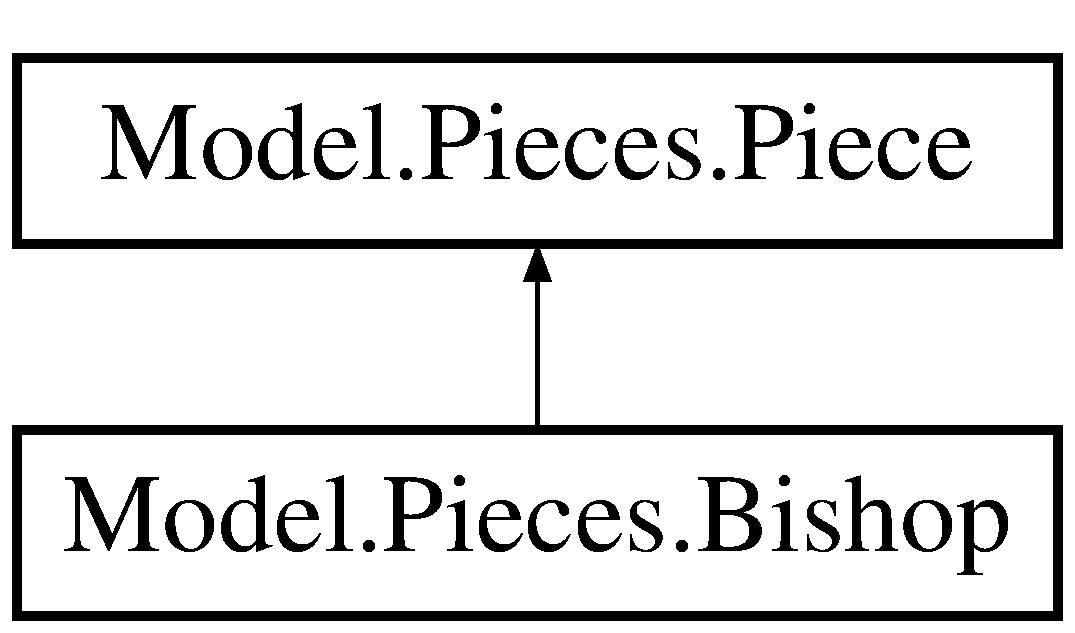
\includegraphics[height=2.000000cm]{class_model_1_1_pieces_1_1_bishop}
\end{center}
\end{figure}
\subsection*{Public Member Functions}
\begin{DoxyCompactItemize}
\item 
\hyperlink{class_model_1_1_pieces_1_1_bishop_a5f383759e28a0def1f6139861c9afa94}{Bishop} (\hyperlink{class_model_1_1_team}{Team} team, int x\+Value, int y\+Value)
\item 
boolean \hyperlink{class_model_1_1_pieces_1_1_bishop_a7767730f9b26965b39385080947c0f6a}{is\+Valid\+Move} (\hyperlink{class_model_1_1_move}{Move} move, \hyperlink{class_model_1_1_board}{Board} board)
\item 
boolean \hyperlink{class_model_1_1_pieces_1_1_bishop_a5d2d653911307254ade5f9b25b4afaf7}{has\+No\+Piece\+In\+Movement\+Route} (\hyperlink{class_model_1_1_move}{Move} move, \hyperlink{class_model_1_1_board}{Board} board)
\item 
List$<$ \hyperlink{class_model_1_1_move}{Move} $>$ \hyperlink{class_model_1_1_pieces_1_1_bishop_a67fdc956c6f82e0b513aae4b86998b28}{find\+All\+Moves} (\hyperlink{class_model_1_1_board}{Board} board)
\end{DoxyCompactItemize}


\subsection{Detailed Description}
\hyperlink{class_model_1_1_pieces_1_1_bishop}{Bishop} class to describe \hyperlink{class_model_1_1_pieces_1_1_bishop}{Bishop}\textquotesingle{}s possible moves. \begin{DoxyAuthor}{Author}
arnavmishra 
\end{DoxyAuthor}


\subsection{Constructor \& Destructor Documentation}
\hypertarget{class_model_1_1_pieces_1_1_bishop_a5f383759e28a0def1f6139861c9afa94}{}\label{class_model_1_1_pieces_1_1_bishop_a5f383759e28a0def1f6139861c9afa94} 
\index{Model\+::\+Pieces\+::\+Bishop@{Model\+::\+Pieces\+::\+Bishop}!Bishop@{Bishop}}
\index{Bishop@{Bishop}!Model\+::\+Pieces\+::\+Bishop@{Model\+::\+Pieces\+::\+Bishop}}
\subsubsection{\texorpdfstring{Bishop()}{Bishop()}}
{\footnotesize\ttfamily Model.\+Pieces.\+Bishop.\+Bishop (\begin{DoxyParamCaption}\item[{\hyperlink{class_model_1_1_team}{Team}}]{team,  }\item[{int}]{x\+Value,  }\item[{int}]{y\+Value }\end{DoxyParamCaption})}

Constructor to initialize \hyperlink{class_model_1_1_pieces_1_1_bishop}{Bishop} on a team and coordinate. 
\begin{DoxyParams}{Parameters}
{\em team} & \\
\hline
\end{DoxyParams}


\subsection{Member Function Documentation}
\hypertarget{class_model_1_1_pieces_1_1_bishop_a67fdc956c6f82e0b513aae4b86998b28}{}\label{class_model_1_1_pieces_1_1_bishop_a67fdc956c6f82e0b513aae4b86998b28} 
\index{Model\+::\+Pieces\+::\+Bishop@{Model\+::\+Pieces\+::\+Bishop}!find\+All\+Moves@{find\+All\+Moves}}
\index{find\+All\+Moves@{find\+All\+Moves}!Model\+::\+Pieces\+::\+Bishop@{Model\+::\+Pieces\+::\+Bishop}}
\subsubsection{\texorpdfstring{find\+All\+Moves()}{findAllMoves()}}
{\footnotesize\ttfamily List$<$\hyperlink{class_model_1_1_move}{Move}$>$ Model.\+Pieces.\+Bishop.\+find\+All\+Moves (\begin{DoxyParamCaption}\item[{\hyperlink{class_model_1_1_board}{Board}}]{board }\end{DoxyParamCaption})}

Function to get all valid possible moves for the bishop in any direction. 
\begin{DoxyParams}{Parameters}
{\em board} & \\
\hline
\end{DoxyParams}
\begin{DoxyReturn}{Returns}
all possible valid moves. 
\end{DoxyReturn}
\hypertarget{class_model_1_1_pieces_1_1_bishop_a5d2d653911307254ade5f9b25b4afaf7}{}\label{class_model_1_1_pieces_1_1_bishop_a5d2d653911307254ade5f9b25b4afaf7} 
\index{Model\+::\+Pieces\+::\+Bishop@{Model\+::\+Pieces\+::\+Bishop}!has\+No\+Piece\+In\+Movement\+Route@{has\+No\+Piece\+In\+Movement\+Route}}
\index{has\+No\+Piece\+In\+Movement\+Route@{has\+No\+Piece\+In\+Movement\+Route}!Model\+::\+Pieces\+::\+Bishop@{Model\+::\+Pieces\+::\+Bishop}}
\subsubsection{\texorpdfstring{has\+No\+Piece\+In\+Movement\+Route()}{hasNoPieceInMovementRoute()}}
{\footnotesize\ttfamily boolean Model.\+Pieces.\+Bishop.\+has\+No\+Piece\+In\+Movement\+Route (\begin{DoxyParamCaption}\item[{\hyperlink{class_model_1_1_move}{Move}}]{move,  }\item[{\hyperlink{class_model_1_1_board}{Board}}]{board }\end{DoxyParamCaption})}

Function to check whether the bishop jumps over any pieces when it moves diagonally. 
\begin{DoxyParams}{Parameters}
{\em move} & \\
\hline
{\em board} & \\
\hline
\end{DoxyParams}
\begin{DoxyReturn}{Returns}
whether the bishop leaps over pieces. 
\end{DoxyReturn}
\hypertarget{class_model_1_1_pieces_1_1_bishop_a7767730f9b26965b39385080947c0f6a}{}\label{class_model_1_1_pieces_1_1_bishop_a7767730f9b26965b39385080947c0f6a} 
\index{Model\+::\+Pieces\+::\+Bishop@{Model\+::\+Pieces\+::\+Bishop}!is\+Valid\+Move@{is\+Valid\+Move}}
\index{is\+Valid\+Move@{is\+Valid\+Move}!Model\+::\+Pieces\+::\+Bishop@{Model\+::\+Pieces\+::\+Bishop}}
\subsubsection{\texorpdfstring{is\+Valid\+Move()}{isValidMove()}}
{\footnotesize\ttfamily boolean Model.\+Pieces.\+Bishop.\+is\+Valid\+Move (\begin{DoxyParamCaption}\item[{\hyperlink{class_model_1_1_move}{Move}}]{move,  }\item[{\hyperlink{class_model_1_1_board}{Board}}]{board }\end{DoxyParamCaption})}

Function to check whether a bishop\textquotesingle{}s move is valid. 
\begin{DoxyParams}{Parameters}
{\em move} & \\
\hline
{\em board} & \\
\hline
\end{DoxyParams}
\begin{DoxyReturn}{Returns}
Whether the move is valid. 
\end{DoxyReturn}


The documentation for this class was generated from the following file\+:\begin{DoxyCompactItemize}
\item 
src/\+Model/\+Pieces/Bishop.\+java\end{DoxyCompactItemize}

\hypertarget{class_tests_1_1_bishop_test}{}\section{Tests.\+Bishop\+Test Class Reference}
\label{class_tests_1_1_bishop_test}\index{Tests.\+Bishop\+Test@{Tests.\+Bishop\+Test}}
\subsection*{Public Member Functions}
\begin{DoxyCompactItemize}
\item 
void \hyperlink{class_tests_1_1_bishop_test_a5966af2d7a4cf4409a7c9e04e14be402}{valid\+Bishop\+Movement} ()  throws Exception 
\item 
void \hyperlink{class_tests_1_1_bishop_test_a3f1b2164ce04847f236b47960a2d6507}{invalid\+Bishop\+Movement} ()  throws Exception 
\item 
void \hyperlink{class_tests_1_1_bishop_test_a1635821930e814400c61693e0e65150c}{correct\+All\+Starting\+Bishop\+Moves} ()  throws Exception 
\end{DoxyCompactItemize}


\subsection{Detailed Description}
Tests for the Bishop Class. \begin{DoxyAuthor}{Author}
arnavmishra 
\end{DoxyAuthor}


\subsection{Member Function Documentation}
\hypertarget{class_tests_1_1_bishop_test_a1635821930e814400c61693e0e65150c}{}\label{class_tests_1_1_bishop_test_a1635821930e814400c61693e0e65150c} 
\index{Tests\+::\+Bishop\+Test@{Tests\+::\+Bishop\+Test}!correct\+All\+Starting\+Bishop\+Moves@{correct\+All\+Starting\+Bishop\+Moves}}
\index{correct\+All\+Starting\+Bishop\+Moves@{correct\+All\+Starting\+Bishop\+Moves}!Tests\+::\+Bishop\+Test@{Tests\+::\+Bishop\+Test}}
\subsubsection{\texorpdfstring{correct\+All\+Starting\+Bishop\+Moves()}{correctAllStartingBishopMoves()}}
{\footnotesize\ttfamily void Tests.\+Bishop\+Test.\+correct\+All\+Starting\+Bishop\+Moves (\begin{DoxyParamCaption}{ }\end{DoxyParamCaption}) throws Exception}

Test to check the bishop\textquotesingle{}s possible movements by moving the pawn diagonally up left from it out of the way and testing to ensure that the bishop can move to all diagonal positions. 
\begin{DoxyExceptions}{Exceptions}
{\em Exception} & \\
\hline
\end{DoxyExceptions}
\hypertarget{class_tests_1_1_bishop_test_a3f1b2164ce04847f236b47960a2d6507}{}\label{class_tests_1_1_bishop_test_a3f1b2164ce04847f236b47960a2d6507} 
\index{Tests\+::\+Bishop\+Test@{Tests\+::\+Bishop\+Test}!invalid\+Bishop\+Movement@{invalid\+Bishop\+Movement}}
\index{invalid\+Bishop\+Movement@{invalid\+Bishop\+Movement}!Tests\+::\+Bishop\+Test@{Tests\+::\+Bishop\+Test}}
\subsubsection{\texorpdfstring{invalid\+Bishop\+Movement()}{invalidBishopMovement()}}
{\footnotesize\ttfamily void Tests.\+Bishop\+Test.\+invalid\+Bishop\+Movement (\begin{DoxyParamCaption}{ }\end{DoxyParamCaption}) throws Exception}

Test to check bishop\textquotesingle{}s invalid movement by moving the pawn in front of it and testing to ensure the bishop cannot move forward. 
\begin{DoxyExceptions}{Exceptions}
{\em Exception} & \\
\hline
\end{DoxyExceptions}
\hypertarget{class_tests_1_1_bishop_test_a5966af2d7a4cf4409a7c9e04e14be402}{}\label{class_tests_1_1_bishop_test_a5966af2d7a4cf4409a7c9e04e14be402} 
\index{Tests\+::\+Bishop\+Test@{Tests\+::\+Bishop\+Test}!valid\+Bishop\+Movement@{valid\+Bishop\+Movement}}
\index{valid\+Bishop\+Movement@{valid\+Bishop\+Movement}!Tests\+::\+Bishop\+Test@{Tests\+::\+Bishop\+Test}}
\subsubsection{\texorpdfstring{valid\+Bishop\+Movement()}{validBishopMovement()}}
{\footnotesize\ttfamily void Tests.\+Bishop\+Test.\+valid\+Bishop\+Movement (\begin{DoxyParamCaption}{ }\end{DoxyParamCaption}) throws Exception}

Test to check the bishop\textquotesingle{}s valid movement by moving the pawn that is diagonally to the left up from it and then moving the bishop in that direction. 
\begin{DoxyExceptions}{Exceptions}
{\em Exception} & \\
\hline
\end{DoxyExceptions}


The documentation for this class was generated from the following file\+:\begin{DoxyCompactItemize}
\item 
src/\+Tests/Bishop\+Test.\+java\end{DoxyCompactItemize}

\hypertarget{class_model_1_1_board}{}\section{Model.\+Board Class Reference}
\label{class_model_1_1_board}\index{Model.\+Board@{Model.\+Board}}
\subsection*{Public Member Functions}
\begin{DoxyCompactItemize}
\item 
\hyperlink{class_model_1_1_board_a9deb765ab1477d72b1674de48a9a6584}{Board} (int width, int length)
\item 
int \hyperlink{class_model_1_1_board_ab6dc3bc9760045e82fa57053f816649f}{get\+Width} ()
\item 
void \hyperlink{class_model_1_1_board_a57a6550786751e1b80fee7552a9355b6}{set\+Width} (int width)
\item 
int \hyperlink{class_model_1_1_board_a35e5cb89e9ade67a786764d0466adecf}{get\+Length} ()
\item 
void \hyperlink{class_model_1_1_board_a189aa2f23e52d961f2cb7f39f584e0a6}{set\+Length} (int length)
\item 
void \hyperlink{class_model_1_1_board_aae76066ac44573318ad06038bcd1cf8e}{set\+Initial\+Board} ()
\item 
void \hyperlink{class_model_1_1_board_aabff4443881dcd377b3a51b06ef5a757}{add\+Piece\+To\+Board} (\hyperlink{class_model_1_1_pieces_1_1_piece}{Piece} piece)
\item 
\hyperlink{class_model_1_1_pieces_1_1_piece}{Piece} \mbox{[}$\,$\mbox{]} \hyperlink{class_model_1_1_board_a2a1d724b1cfaa4ec61b22e6d6b769cab}{set\+Primary\+Pieces} (\hyperlink{class_model_1_1_pieces_1_1_piece}{Piece}\mbox{[}$\,$\mbox{]}\mbox{[}$\,$\mbox{]} positions, int y\+Value, \hyperlink{class_model_1_1_team}{Team} team)
\item 
\hyperlink{class_model_1_1_pieces_1_1_piece}{Piece} \mbox{[}$\,$\mbox{]}\mbox{[}$\,$\mbox{]} \hyperlink{class_model_1_1_board_a6d51fda7af5f561f6bd1478e2411d3bd}{get\+Positions} ()
\item 
\hyperlink{class_model_1_1_pieces_1_1_piece}{Piece} \hyperlink{class_model_1_1_board_aec81a53097f16fadf2d64dab72cf6d47}{set\+Positions} (\hyperlink{class_model_1_1_move}{Move} move)
\item 
void \hyperlink{class_model_1_1_board_a6c918896308d9752d1e81989766c6bee}{unset\+Positions} (\hyperlink{class_model_1_1_move}{Move} move, \hyperlink{class_model_1_1_pieces_1_1_piece}{Piece} removed)
\item 
boolean \hyperlink{class_model_1_1_board_a9d041c45865ca1db8ff39c9f4fce204e}{is\+Team\+In\+Check} (\hyperlink{class_model_1_1_move}{Move} move)
\item 
boolean \hyperlink{class_model_1_1_board_a16886f1ae73fae80ffbd439cda934e8a}{get\+Check\+Mate} (int turn\+Team\+Number)
\item 
boolean \hyperlink{class_model_1_1_board_a6a8d2dc192be22d581618ac2b3301966}{get\+Stale\+Mate} (int turn\+Team\+Number)
\item 
\hyperlink{class_model_1_1_pieces_1_1_piece}{Piece} \hyperlink{class_model_1_1_board_a0513468651fe1afccc197f700e2c760d}{get\+King} (List$<$ \hyperlink{class_model_1_1_pieces_1_1_piece}{Piece} $>$ pieces)
\item 
int \hyperlink{class_model_1_1_board_a6fac52f7cf767e242f6d202a9e52eb8c}{toggle\+Team} (int turn\+Team\+Number)
\item 
\hyperlink{class_model_1_1_team}{Team} \hyperlink{class_model_1_1_board_afbbd0336890f96410b94a622290db60d}{get\+Team} (int turn\+Team\+Number)
\item 
List$<$ \hyperlink{class_model_1_1_pieces_1_1_piece}{Piece} $>$ \hyperlink{class_model_1_1_board_abce1029b057dce2939f5dd78abad3cec}{get\+Team\+Pieces} (int turn\+Team\+Number)
\item 
void \hyperlink{class_model_1_1_board_a07633635c4378b1824a69deddfb521d5}{print\+Board} ()
\item 
void \hyperlink{class_model_1_1_board_a79dabcf1688b67bac808be8c67364bce}{print\+Piece} (\hyperlink{class_model_1_1_pieces_1_1_piece}{Piece} piece)
\end{DoxyCompactItemize}


\subsection{Detailed Description}
The board class describes the details about the board and a snapshot of the current game play including piece positions and team statuses. \begin{DoxyAuthor}{Author}
arnavmishra 
\end{DoxyAuthor}


\subsection{Constructor \& Destructor Documentation}
\hypertarget{class_model_1_1_board_a9deb765ab1477d72b1674de48a9a6584}{}\label{class_model_1_1_board_a9deb765ab1477d72b1674de48a9a6584} 
\index{Model\+::\+Board@{Model\+::\+Board}!Board@{Board}}
\index{Board@{Board}!Model\+::\+Board@{Model\+::\+Board}}
\subsubsection{\texorpdfstring{Board()}{Board()}}
{\footnotesize\ttfamily Model.\+Board.\+Board (\begin{DoxyParamCaption}\item[{int}]{width,  }\item[{int}]{length }\end{DoxyParamCaption})}

\hyperlink{class_model_1_1_board}{Board} constructor to set up initial board piece positions and the width and length. 
\begin{DoxyParams}{Parameters}
{\em width} & \\
\hline
{\em length} & \\
\hline
\end{DoxyParams}


\subsection{Member Function Documentation}
\hypertarget{class_model_1_1_board_aabff4443881dcd377b3a51b06ef5a757}{}\label{class_model_1_1_board_aabff4443881dcd377b3a51b06ef5a757} 
\index{Model\+::\+Board@{Model\+::\+Board}!add\+Piece\+To\+Board@{add\+Piece\+To\+Board}}
\index{add\+Piece\+To\+Board@{add\+Piece\+To\+Board}!Model\+::\+Board@{Model\+::\+Board}}
\subsubsection{\texorpdfstring{add\+Piece\+To\+Board()}{addPieceToBoard()}}
{\footnotesize\ttfamily void Model.\+Board.\+add\+Piece\+To\+Board (\begin{DoxyParamCaption}\item[{\hyperlink{class_model_1_1_pieces_1_1_piece}{Piece}}]{piece }\end{DoxyParamCaption})}

Function to add a new piece to a specified coordinate on the board regardless of whether or not another piece exists there. 
\begin{DoxyParams}{Parameters}
{\em piece} & \\
\hline
\end{DoxyParams}
\hypertarget{class_model_1_1_board_a16886f1ae73fae80ffbd439cda934e8a}{}\label{class_model_1_1_board_a16886f1ae73fae80ffbd439cda934e8a} 
\index{Model\+::\+Board@{Model\+::\+Board}!get\+Check\+Mate@{get\+Check\+Mate}}
\index{get\+Check\+Mate@{get\+Check\+Mate}!Model\+::\+Board@{Model\+::\+Board}}
\subsubsection{\texorpdfstring{get\+Check\+Mate()}{getCheckMate()}}
{\footnotesize\ttfamily boolean Model.\+Board.\+get\+Check\+Mate (\begin{DoxyParamCaption}\item[{int}]{turn\+Team\+Number }\end{DoxyParamCaption})}

Method to see if a move called a checkmate. 
\begin{DoxyParams}{Parameters}
{\em turn\+Team\+Number} & \\
\hline
\end{DoxyParams}
\begin{DoxyReturn}{Returns}
whether the team is in checkmate. 
\end{DoxyReturn}
\hypertarget{class_model_1_1_board_a0513468651fe1afccc197f700e2c760d}{}\label{class_model_1_1_board_a0513468651fe1afccc197f700e2c760d} 
\index{Model\+::\+Board@{Model\+::\+Board}!get\+King@{get\+King}}
\index{get\+King@{get\+King}!Model\+::\+Board@{Model\+::\+Board}}
\subsubsection{\texorpdfstring{get\+King()}{getKing()}}
{\footnotesize\ttfamily \hyperlink{class_model_1_1_pieces_1_1_piece}{Piece} Model.\+Board.\+get\+King (\begin{DoxyParamCaption}\item[{List$<$ \hyperlink{class_model_1_1_pieces_1_1_piece}{Piece} $>$}]{pieces }\end{DoxyParamCaption})}

Helper function to get the King from a list of pieces. 
\begin{DoxyParams}{Parameters}
{\em pieces} & \\
\hline
\end{DoxyParams}
\begin{DoxyReturn}{Returns}
King\textquotesingle{}s piece 
\end{DoxyReturn}
\hypertarget{class_model_1_1_board_a35e5cb89e9ade67a786764d0466adecf}{}\label{class_model_1_1_board_a35e5cb89e9ade67a786764d0466adecf} 
\index{Model\+::\+Board@{Model\+::\+Board}!get\+Length@{get\+Length}}
\index{get\+Length@{get\+Length}!Model\+::\+Board@{Model\+::\+Board}}
\subsubsection{\texorpdfstring{get\+Length()}{getLength()}}
{\footnotesize\ttfamily int Model.\+Board.\+get\+Length (\begin{DoxyParamCaption}{ }\end{DoxyParamCaption})}

Get length of board. \begin{DoxyReturn}{Returns}
length 
\end{DoxyReturn}
\hypertarget{class_model_1_1_board_a6d51fda7af5f561f6bd1478e2411d3bd}{}\label{class_model_1_1_board_a6d51fda7af5f561f6bd1478e2411d3bd} 
\index{Model\+::\+Board@{Model\+::\+Board}!get\+Positions@{get\+Positions}}
\index{get\+Positions@{get\+Positions}!Model\+::\+Board@{Model\+::\+Board}}
\subsubsection{\texorpdfstring{get\+Positions()}{getPositions()}}
{\footnotesize\ttfamily \hyperlink{class_model_1_1_pieces_1_1_piece}{Piece} \mbox{[}$\,$\mbox{]}\mbox{[}$\,$\mbox{]} Model.\+Board.\+get\+Positions (\begin{DoxyParamCaption}{ }\end{DoxyParamCaption})}

Get positions on entire chess board. \begin{DoxyReturn}{Returns}
positions 
\end{DoxyReturn}
\hypertarget{class_model_1_1_board_a6a8d2dc192be22d581618ac2b3301966}{}\label{class_model_1_1_board_a6a8d2dc192be22d581618ac2b3301966} 
\index{Model\+::\+Board@{Model\+::\+Board}!get\+Stale\+Mate@{get\+Stale\+Mate}}
\index{get\+Stale\+Mate@{get\+Stale\+Mate}!Model\+::\+Board@{Model\+::\+Board}}
\subsubsection{\texorpdfstring{get\+Stale\+Mate()}{getStaleMate()}}
{\footnotesize\ttfamily boolean Model.\+Board.\+get\+Stale\+Mate (\begin{DoxyParamCaption}\item[{int}]{turn\+Team\+Number }\end{DoxyParamCaption})}

Method to see if a team cannot move any piece in which case the game is in a stale mate. 
\begin{DoxyParams}{Parameters}
{\em turn\+Team\+Number} & \\
\hline
\end{DoxyParams}
\begin{DoxyReturn}{Returns}

\end{DoxyReturn}
\hypertarget{class_model_1_1_board_afbbd0336890f96410b94a622290db60d}{}\label{class_model_1_1_board_afbbd0336890f96410b94a622290db60d} 
\index{Model\+::\+Board@{Model\+::\+Board}!get\+Team@{get\+Team}}
\index{get\+Team@{get\+Team}!Model\+::\+Board@{Model\+::\+Board}}
\subsubsection{\texorpdfstring{get\+Team()}{getTeam()}}
{\footnotesize\ttfamily \hyperlink{class_model_1_1_team}{Team} Model.\+Board.\+get\+Team (\begin{DoxyParamCaption}\item[{int}]{turn\+Team\+Number }\end{DoxyParamCaption})}

Helper function to return a team object given a team number. 
\begin{DoxyParams}{Parameters}
{\em turn\+Team\+Number} & \\
\hline
\end{DoxyParams}
\begin{DoxyReturn}{Returns}
team\textquotesingle{}s active pieces. 
\end{DoxyReturn}
\hypertarget{class_model_1_1_board_abce1029b057dce2939f5dd78abad3cec}{}\label{class_model_1_1_board_abce1029b057dce2939f5dd78abad3cec} 
\index{Model\+::\+Board@{Model\+::\+Board}!get\+Team\+Pieces@{get\+Team\+Pieces}}
\index{get\+Team\+Pieces@{get\+Team\+Pieces}!Model\+::\+Board@{Model\+::\+Board}}
\subsubsection{\texorpdfstring{get\+Team\+Pieces()}{getTeamPieces()}}
{\footnotesize\ttfamily List$<$\hyperlink{class_model_1_1_pieces_1_1_piece}{Piece}$>$ Model.\+Board.\+get\+Team\+Pieces (\begin{DoxyParamCaption}\item[{int}]{turn\+Team\+Number }\end{DoxyParamCaption})}

Helper function to return the remaining pieces of a team 
\begin{DoxyParams}{Parameters}
{\em turn\+Team\+Number} & \\
\hline
\end{DoxyParams}
\begin{DoxyReturn}{Returns}

\end{DoxyReturn}
\hypertarget{class_model_1_1_board_ab6dc3bc9760045e82fa57053f816649f}{}\label{class_model_1_1_board_ab6dc3bc9760045e82fa57053f816649f} 
\index{Model\+::\+Board@{Model\+::\+Board}!get\+Width@{get\+Width}}
\index{get\+Width@{get\+Width}!Model\+::\+Board@{Model\+::\+Board}}
\subsubsection{\texorpdfstring{get\+Width()}{getWidth()}}
{\footnotesize\ttfamily int Model.\+Board.\+get\+Width (\begin{DoxyParamCaption}{ }\end{DoxyParamCaption})}

Get width of board. \begin{DoxyReturn}{Returns}
width 
\end{DoxyReturn}
\hypertarget{class_model_1_1_board_a9d041c45865ca1db8ff39c9f4fce204e}{}\label{class_model_1_1_board_a9d041c45865ca1db8ff39c9f4fce204e} 
\index{Model\+::\+Board@{Model\+::\+Board}!is\+Team\+In\+Check@{is\+Team\+In\+Check}}
\index{is\+Team\+In\+Check@{is\+Team\+In\+Check}!Model\+::\+Board@{Model\+::\+Board}}
\subsubsection{\texorpdfstring{is\+Team\+In\+Check()}{isTeamInCheck()}}
{\footnotesize\ttfamily boolean Model.\+Board.\+is\+Team\+In\+Check (\begin{DoxyParamCaption}\item[{\hyperlink{class_model_1_1_move}{Move}}]{move }\end{DoxyParamCaption})}

Method to see if the king will still be in check after the move is made. Undo the move after. 
\begin{DoxyParams}{Parameters}
{\em move} & \\
\hline
\end{DoxyParams}
\begin{DoxyReturn}{Returns}
whether the king is in check after the move. 
\end{DoxyReturn}
\hypertarget{class_model_1_1_board_a07633635c4378b1824a69deddfb521d5}{}\label{class_model_1_1_board_a07633635c4378b1824a69deddfb521d5} 
\index{Model\+::\+Board@{Model\+::\+Board}!print\+Board@{print\+Board}}
\index{print\+Board@{print\+Board}!Model\+::\+Board@{Model\+::\+Board}}
\subsubsection{\texorpdfstring{print\+Board()}{printBoard()}}
{\footnotesize\ttfamily void Model.\+Board.\+print\+Board (\begin{DoxyParamCaption}{ }\end{DoxyParamCaption})}

Function to print out board. Everything below this is simply for testing purposes and will be removed when the G\+UI is done. 
\begin{DoxyParams}{Parameters}
{\em board} & \\
\hline
\end{DoxyParams}
\hypertarget{class_model_1_1_board_a79dabcf1688b67bac808be8c67364bce}{}\label{class_model_1_1_board_a79dabcf1688b67bac808be8c67364bce} 
\index{Model\+::\+Board@{Model\+::\+Board}!print\+Piece@{print\+Piece}}
\index{print\+Piece@{print\+Piece}!Model\+::\+Board@{Model\+::\+Board}}
\subsubsection{\texorpdfstring{print\+Piece()}{printPiece()}}
{\footnotesize\ttfamily void Model.\+Board.\+print\+Piece (\begin{DoxyParamCaption}\item[{\hyperlink{class_model_1_1_pieces_1_1_piece}{Piece}}]{piece }\end{DoxyParamCaption})}

Helper function to print out each piece on the board. 
\begin{DoxyParams}{Parameters}
{\em piece} & \\
\hline
\end{DoxyParams}
\hypertarget{class_model_1_1_board_aae76066ac44573318ad06038bcd1cf8e}{}\label{class_model_1_1_board_aae76066ac44573318ad06038bcd1cf8e} 
\index{Model\+::\+Board@{Model\+::\+Board}!set\+Initial\+Board@{set\+Initial\+Board}}
\index{set\+Initial\+Board@{set\+Initial\+Board}!Model\+::\+Board@{Model\+::\+Board}}
\subsubsection{\texorpdfstring{set\+Initial\+Board()}{setInitialBoard()}}
{\footnotesize\ttfamily void Model.\+Board.\+set\+Initial\+Board (\begin{DoxyParamCaption}{ }\end{DoxyParamCaption})}

Function to put pieces in initial starting positions. \begin{DoxyReturn}{Returns}
a Piece double array with all the current positions. 
\end{DoxyReturn}
\hypertarget{class_model_1_1_board_a189aa2f23e52d961f2cb7f39f584e0a6}{}\label{class_model_1_1_board_a189aa2f23e52d961f2cb7f39f584e0a6} 
\index{Model\+::\+Board@{Model\+::\+Board}!set\+Length@{set\+Length}}
\index{set\+Length@{set\+Length}!Model\+::\+Board@{Model\+::\+Board}}
\subsubsection{\texorpdfstring{set\+Length()}{setLength()}}
{\footnotesize\ttfamily void Model.\+Board.\+set\+Length (\begin{DoxyParamCaption}\item[{int}]{length }\end{DoxyParamCaption})}

Set length of board. 
\begin{DoxyParams}{Parameters}
{\em length} & \\
\hline
\end{DoxyParams}
\hypertarget{class_model_1_1_board_aec81a53097f16fadf2d64dab72cf6d47}{}\label{class_model_1_1_board_aec81a53097f16fadf2d64dab72cf6d47} 
\index{Model\+::\+Board@{Model\+::\+Board}!set\+Positions@{set\+Positions}}
\index{set\+Positions@{set\+Positions}!Model\+::\+Board@{Model\+::\+Board}}
\subsubsection{\texorpdfstring{set\+Positions()}{setPositions()}}
{\footnotesize\ttfamily \hyperlink{class_model_1_1_pieces_1_1_piece}{Piece} Model.\+Board.\+set\+Positions (\begin{DoxyParamCaption}\item[{\hyperlink{class_model_1_1_move}{Move}}]{move }\end{DoxyParamCaption})}

Set the new positions of a chess board after a move. 
\begin{DoxyParams}{Parameters}
{\em move} & \\
\hline
\end{DoxyParams}
\hypertarget{class_model_1_1_board_a2a1d724b1cfaa4ec61b22e6d6b769cab}{}\label{class_model_1_1_board_a2a1d724b1cfaa4ec61b22e6d6b769cab} 
\index{Model\+::\+Board@{Model\+::\+Board}!set\+Primary\+Pieces@{set\+Primary\+Pieces}}
\index{set\+Primary\+Pieces@{set\+Primary\+Pieces}!Model\+::\+Board@{Model\+::\+Board}}
\subsubsection{\texorpdfstring{set\+Primary\+Pieces()}{setPrimaryPieces()}}
{\footnotesize\ttfamily \hyperlink{class_model_1_1_pieces_1_1_piece}{Piece} \mbox{[}$\,$\mbox{]} Model.\+Board.\+set\+Primary\+Pieces (\begin{DoxyParamCaption}\item[{\hyperlink{class_model_1_1_pieces_1_1_piece}{Piece}}]{positions\mbox{[}$\,$\mbox{]}\mbox{[}$\,$\mbox{]},  }\item[{int}]{y\+Value,  }\item[{\hyperlink{class_model_1_1_team}{Team}}]{team }\end{DoxyParamCaption})}

Helper function to initialize all the non-\/pawns and put them in the right places. 
\begin{DoxyParams}{Parameters}
{\em positions} & \\
\hline
{\em y\+Value} & \\
\hline
{\em team} & \\
\hline
\end{DoxyParams}
\begin{DoxyReturn}{Returns}
Pieces 1-\/d array with the primary non-\/pawn pieces for a team. 
\end{DoxyReturn}
\hypertarget{class_model_1_1_board_a57a6550786751e1b80fee7552a9355b6}{}\label{class_model_1_1_board_a57a6550786751e1b80fee7552a9355b6} 
\index{Model\+::\+Board@{Model\+::\+Board}!set\+Width@{set\+Width}}
\index{set\+Width@{set\+Width}!Model\+::\+Board@{Model\+::\+Board}}
\subsubsection{\texorpdfstring{set\+Width()}{setWidth()}}
{\footnotesize\ttfamily void Model.\+Board.\+set\+Width (\begin{DoxyParamCaption}\item[{int}]{width }\end{DoxyParamCaption})}

Set width of board. 
\begin{DoxyParams}{Parameters}
{\em width} & \\
\hline
\end{DoxyParams}
\hypertarget{class_model_1_1_board_a6fac52f7cf767e242f6d202a9e52eb8c}{}\label{class_model_1_1_board_a6fac52f7cf767e242f6d202a9e52eb8c} 
\index{Model\+::\+Board@{Model\+::\+Board}!toggle\+Team@{toggle\+Team}}
\index{toggle\+Team@{toggle\+Team}!Model\+::\+Board@{Model\+::\+Board}}
\subsubsection{\texorpdfstring{toggle\+Team()}{toggleTeam()}}
{\footnotesize\ttfamily int Model.\+Board.\+toggle\+Team (\begin{DoxyParamCaption}\item[{int}]{turn\+Team\+Number }\end{DoxyParamCaption})}

Helper function to change the team number. 
\begin{DoxyParams}{Parameters}
{\em turn\+Team\+Number} & \\
\hline
\end{DoxyParams}
\begin{DoxyReturn}{Returns}
opposite team number. 
\end{DoxyReturn}
\hypertarget{class_model_1_1_board_a6c918896308d9752d1e81989766c6bee}{}\label{class_model_1_1_board_a6c918896308d9752d1e81989766c6bee} 
\index{Model\+::\+Board@{Model\+::\+Board}!unset\+Positions@{unset\+Positions}}
\index{unset\+Positions@{unset\+Positions}!Model\+::\+Board@{Model\+::\+Board}}
\subsubsection{\texorpdfstring{unset\+Positions()}{unsetPositions()}}
{\footnotesize\ttfamily void Model.\+Board.\+unset\+Positions (\begin{DoxyParamCaption}\item[{\hyperlink{class_model_1_1_move}{Move}}]{move,  }\item[{\hyperlink{class_model_1_1_pieces_1_1_piece}{Piece}}]{removed }\end{DoxyParamCaption})}

Undo the last move. This method is used to reverse a move after checking if it protects the King from a check. This is relevant when checking for checkmates to ensure that there is at least one move available for the team. 
\begin{DoxyParams}{Parameters}
{\em move} & \\
\hline
{\em removed} & \\
\hline
\end{DoxyParams}


The documentation for this class was generated from the following file\+:\begin{DoxyCompactItemize}
\item 
src/\+Model/Board.\+java\end{DoxyCompactItemize}

\hypertarget{class_tests_1_1_board_test}{}\section{Tests.\+Board\+Test Class Reference}
\label{class_tests_1_1_board_test}\index{Tests.\+Board\+Test@{Tests.\+Board\+Test}}
\subsection*{Public Member Functions}
\begin{DoxyCompactItemize}
\item 
void \hyperlink{class_tests_1_1_board_test_a7a85d67a559913d4e5a3b0977daa5309}{valid\+Constructor} ()  throws Exception 
\item 
void \hyperlink{class_tests_1_1_board_test_acd51124659fb2a0eb4f6fcc9b41e8001}{moving\+Piece} ()  throws Exception 
\item 
void \hyperlink{class_tests_1_1_board_test_a929e0f87bd865f7fdf810ab37768f4e8}{not\+In\+Check} ()  throws Exception 
\item 
void \hyperlink{class_tests_1_1_board_test_aa5b9e4cbefe4702bcd89fbc9ee886a29}{not\+Protecting\+Check} ()  throws Exception 
\item 
void \hyperlink{class_tests_1_1_board_test_a59084580ebe6a2c112887b13c1fa63ee}{protecting\+Check} ()  throws Exception 
\item 
void \hyperlink{class_tests_1_1_board_test_a2e13dc59ccbbdb6535ed634b612b2fb1}{not\+In\+Check\+Mate} ()  throws Exception 
\item 
void \hyperlink{class_tests_1_1_board_test_a39bdcd7eb309f039104f07d042d0678f}{in\+Check\+Mate} ()  throws Exception 
\item 
void \hyperlink{class_tests_1_1_board_test_a33895f492ce1d7dfba81b325fa351da0}{set\+Up\+Check} (\hyperlink{class_framework_1_1_board}{Board} board)
\item 
void \hyperlink{class_tests_1_1_board_test_a403efc830e97a274bc65ea131dfb0e5f}{not\+In\+Stale\+Mate} ()  throws Exception 
\item 
void \hyperlink{class_tests_1_1_board_test_aaa8c24159f5ef9acbb15b47ae83f8d88}{in\+Stale\+Mate} ()  throws Exception 
\item 
void \hyperlink{class_tests_1_1_board_test_a6e66cbfe15e55e7f65f37a85fd8126b2}{set\+Up\+Stale\+Mate} (\hyperlink{class_framework_1_1_board}{Board} board)
\end{DoxyCompactItemize}


\subsection{Detailed Description}
\hyperlink{namespace_tests}{Tests} for the Board class. \begin{DoxyAuthor}{Author}
arnavmishra 
\end{DoxyAuthor}


\subsection{Member Function Documentation}
\hypertarget{class_tests_1_1_board_test_a39bdcd7eb309f039104f07d042d0678f}{}\label{class_tests_1_1_board_test_a39bdcd7eb309f039104f07d042d0678f} 
\index{Tests\+::\+Board\+Test@{Tests\+::\+Board\+Test}!in\+Check\+Mate@{in\+Check\+Mate}}
\index{in\+Check\+Mate@{in\+Check\+Mate}!Tests\+::\+Board\+Test@{Tests\+::\+Board\+Test}}
\subsubsection{\texorpdfstring{in\+Check\+Mate()}{inCheckMate()}}
{\footnotesize\ttfamily void Tests.\+Board\+Test.\+in\+Check\+Mate (\begin{DoxyParamCaption}{ }\end{DoxyParamCaption}) throws Exception}

Test to simulate a checkmate and confirm that the board has the checkmate listed. 
\begin{DoxyExceptions}{Exceptions}
{\em Exception} & \\
\hline
\end{DoxyExceptions}
\hypertarget{class_tests_1_1_board_test_aaa8c24159f5ef9acbb15b47ae83f8d88}{}\label{class_tests_1_1_board_test_aaa8c24159f5ef9acbb15b47ae83f8d88} 
\index{Tests\+::\+Board\+Test@{Tests\+::\+Board\+Test}!in\+Stale\+Mate@{in\+Stale\+Mate}}
\index{in\+Stale\+Mate@{in\+Stale\+Mate}!Tests\+::\+Board\+Test@{Tests\+::\+Board\+Test}}
\subsubsection{\texorpdfstring{in\+Stale\+Mate()}{inStaleMate()}}
{\footnotesize\ttfamily void Tests.\+Board\+Test.\+in\+Stale\+Mate (\begin{DoxyParamCaption}{ }\end{DoxyParamCaption}) throws Exception}

Test to check stalemate to confirm that when no piece can move, the board stops for stalemate. 
\begin{DoxyExceptions}{Exceptions}
{\em Exception} & \\
\hline
\end{DoxyExceptions}
\hypertarget{class_tests_1_1_board_test_acd51124659fb2a0eb4f6fcc9b41e8001}{}\label{class_tests_1_1_board_test_acd51124659fb2a0eb4f6fcc9b41e8001} 
\index{Tests\+::\+Board\+Test@{Tests\+::\+Board\+Test}!moving\+Piece@{moving\+Piece}}
\index{moving\+Piece@{moving\+Piece}!Tests\+::\+Board\+Test@{Tests\+::\+Board\+Test}}
\subsubsection{\texorpdfstring{moving\+Piece()}{movingPiece()}}
{\footnotesize\ttfamily void Tests.\+Board\+Test.\+moving\+Piece (\begin{DoxyParamCaption}{ }\end{DoxyParamCaption}) throws Exception}

Test for piece movement where a pawn is moved forward and then the board is checked to confirm that the pawn is now in the new location. 
\begin{DoxyExceptions}{Exceptions}
{\em Exception} & \\
\hline
\end{DoxyExceptions}
\hypertarget{class_tests_1_1_board_test_a929e0f87bd865f7fdf810ab37768f4e8}{}\label{class_tests_1_1_board_test_a929e0f87bd865f7fdf810ab37768f4e8} 
\index{Tests\+::\+Board\+Test@{Tests\+::\+Board\+Test}!not\+In\+Check@{not\+In\+Check}}
\index{not\+In\+Check@{not\+In\+Check}!Tests\+::\+Board\+Test@{Tests\+::\+Board\+Test}}
\subsubsection{\texorpdfstring{not\+In\+Check()}{notInCheck()}}
{\footnotesize\ttfamily void Tests.\+Board\+Test.\+not\+In\+Check (\begin{DoxyParamCaption}{ }\end{DoxyParamCaption}) throws Exception}

Test to see if the board is not in check. This is done using the initial board setup and ensuring that the team\textquotesingle{}s are not in check with a simple movement such as moving a pawn forward. 
\begin{DoxyExceptions}{Exceptions}
{\em Exception} & \\
\hline
\end{DoxyExceptions}
\hypertarget{class_tests_1_1_board_test_a2e13dc59ccbbdb6535ed634b612b2fb1}{}\label{class_tests_1_1_board_test_a2e13dc59ccbbdb6535ed634b612b2fb1} 
\index{Tests\+::\+Board\+Test@{Tests\+::\+Board\+Test}!not\+In\+Check\+Mate@{not\+In\+Check\+Mate}}
\index{not\+In\+Check\+Mate@{not\+In\+Check\+Mate}!Tests\+::\+Board\+Test@{Tests\+::\+Board\+Test}}
\subsubsection{\texorpdfstring{not\+In\+Check\+Mate()}{notInCheckMate()}}
{\footnotesize\ttfamily void Tests.\+Board\+Test.\+not\+In\+Check\+Mate (\begin{DoxyParamCaption}{ }\end{DoxyParamCaption}) throws Exception}

Test to check when the board is not in Check\+Mate by using the initial board setup. 
\begin{DoxyExceptions}{Exceptions}
{\em Exception} & \\
\hline
\end{DoxyExceptions}
\hypertarget{class_tests_1_1_board_test_a403efc830e97a274bc65ea131dfb0e5f}{}\label{class_tests_1_1_board_test_a403efc830e97a274bc65ea131dfb0e5f} 
\index{Tests\+::\+Board\+Test@{Tests\+::\+Board\+Test}!not\+In\+Stale\+Mate@{not\+In\+Stale\+Mate}}
\index{not\+In\+Stale\+Mate@{not\+In\+Stale\+Mate}!Tests\+::\+Board\+Test@{Tests\+::\+Board\+Test}}
\subsubsection{\texorpdfstring{not\+In\+Stale\+Mate()}{notInStaleMate()}}
{\footnotesize\ttfamily void Tests.\+Board\+Test.\+not\+In\+Stale\+Mate (\begin{DoxyParamCaption}{ }\end{DoxyParamCaption}) throws Exception}

Test to check that the game is not in stalemate by using the initial board setup. 
\begin{DoxyExceptions}{Exceptions}
{\em Exception} & \\
\hline
\end{DoxyExceptions}
\hypertarget{class_tests_1_1_board_test_aa5b9e4cbefe4702bcd89fbc9ee886a29}{}\label{class_tests_1_1_board_test_aa5b9e4cbefe4702bcd89fbc9ee886a29} 
\index{Tests\+::\+Board\+Test@{Tests\+::\+Board\+Test}!not\+Protecting\+Check@{not\+Protecting\+Check}}
\index{not\+Protecting\+Check@{not\+Protecting\+Check}!Tests\+::\+Board\+Test@{Tests\+::\+Board\+Test}}
\subsubsection{\texorpdfstring{not\+Protecting\+Check()}{notProtectingCheck()}}
{\footnotesize\ttfamily void Tests.\+Board\+Test.\+not\+Protecting\+Check (\begin{DoxyParamCaption}{ }\end{DoxyParamCaption}) throws Exception}

Test to confirm that the team is still in check if a team does not move to prevent the current check. 
\begin{DoxyExceptions}{Exceptions}
{\em Exception} & \\
\hline
\end{DoxyExceptions}
\hypertarget{class_tests_1_1_board_test_a59084580ebe6a2c112887b13c1fa63ee}{}\label{class_tests_1_1_board_test_a59084580ebe6a2c112887b13c1fa63ee} 
\index{Tests\+::\+Board\+Test@{Tests\+::\+Board\+Test}!protecting\+Check@{protecting\+Check}}
\index{protecting\+Check@{protecting\+Check}!Tests\+::\+Board\+Test@{Tests\+::\+Board\+Test}}
\subsubsection{\texorpdfstring{protecting\+Check()}{protectingCheck()}}
{\footnotesize\ttfamily void Tests.\+Board\+Test.\+protecting\+Check (\begin{DoxyParamCaption}{ }\end{DoxyParamCaption}) throws Exception}

Test to confirm that after moving a piece in the way of a check, the check is no longer there. 
\begin{DoxyExceptions}{Exceptions}
{\em Exception} & \\
\hline
\end{DoxyExceptions}
\hypertarget{class_tests_1_1_board_test_a33895f492ce1d7dfba81b325fa351da0}{}\label{class_tests_1_1_board_test_a33895f492ce1d7dfba81b325fa351da0} 
\index{Tests\+::\+Board\+Test@{Tests\+::\+Board\+Test}!set\+Up\+Check@{set\+Up\+Check}}
\index{set\+Up\+Check@{set\+Up\+Check}!Tests\+::\+Board\+Test@{Tests\+::\+Board\+Test}}
\subsubsection{\texorpdfstring{set\+Up\+Check()}{setUpCheck()}}
{\footnotesize\ttfamily void Tests.\+Board\+Test.\+set\+Up\+Check (\begin{DoxyParamCaption}\item[{\hyperlink{class_framework_1_1_board}{Board}}]{board }\end{DoxyParamCaption})}

Helper function to set up a board into a check situation. 
\begin{DoxyParams}{Parameters}
{\em board} & \\
\hline
\end{DoxyParams}
\hypertarget{class_tests_1_1_board_test_a6e66cbfe15e55e7f65f37a85fd8126b2}{}\label{class_tests_1_1_board_test_a6e66cbfe15e55e7f65f37a85fd8126b2} 
\index{Tests\+::\+Board\+Test@{Tests\+::\+Board\+Test}!set\+Up\+Stale\+Mate@{set\+Up\+Stale\+Mate}}
\index{set\+Up\+Stale\+Mate@{set\+Up\+Stale\+Mate}!Tests\+::\+Board\+Test@{Tests\+::\+Board\+Test}}
\subsubsection{\texorpdfstring{set\+Up\+Stale\+Mate()}{setUpStaleMate()}}
{\footnotesize\ttfamily void Tests.\+Board\+Test.\+set\+Up\+Stale\+Mate (\begin{DoxyParamCaption}\item[{\hyperlink{class_framework_1_1_board}{Board}}]{board }\end{DoxyParamCaption})}

Helper function to set up a stalemate. 
\begin{DoxyParams}{Parameters}
{\em board} & \\
\hline
\end{DoxyParams}
\hypertarget{class_tests_1_1_board_test_a7a85d67a559913d4e5a3b0977daa5309}{}\label{class_tests_1_1_board_test_a7a85d67a559913d4e5a3b0977daa5309} 
\index{Tests\+::\+Board\+Test@{Tests\+::\+Board\+Test}!valid\+Constructor@{valid\+Constructor}}
\index{valid\+Constructor@{valid\+Constructor}!Tests\+::\+Board\+Test@{Tests\+::\+Board\+Test}}
\subsubsection{\texorpdfstring{valid\+Constructor()}{validConstructor()}}
{\footnotesize\ttfamily void Tests.\+Board\+Test.\+valid\+Constructor (\begin{DoxyParamCaption}{ }\end{DoxyParamCaption}) throws Exception}

Test for the Board constructor to ensure that the width and length are properly set. 
\begin{DoxyExceptions}{Exceptions}
{\em Exception} & \\
\hline
\end{DoxyExceptions}


The documentation for this class was generated from the following file\+:\begin{DoxyCompactItemize}
\item 
src/\+Tests/\hyperlink{_board_test_8java}{Board\+Test.\+java}\end{DoxyCompactItemize}

\hypertarget{class_model_1_1_pieces_1_1_checker}{}\section{Model.\+Pieces.\+Checker Class Reference}
\label{class_model_1_1_pieces_1_1_checker}\index{Model.\+Pieces.\+Checker@{Model.\+Pieces.\+Checker}}
Inheritance diagram for Model.\+Pieces.\+Checker\+:\begin{figure}[H]
\begin{center}
\leavevmode
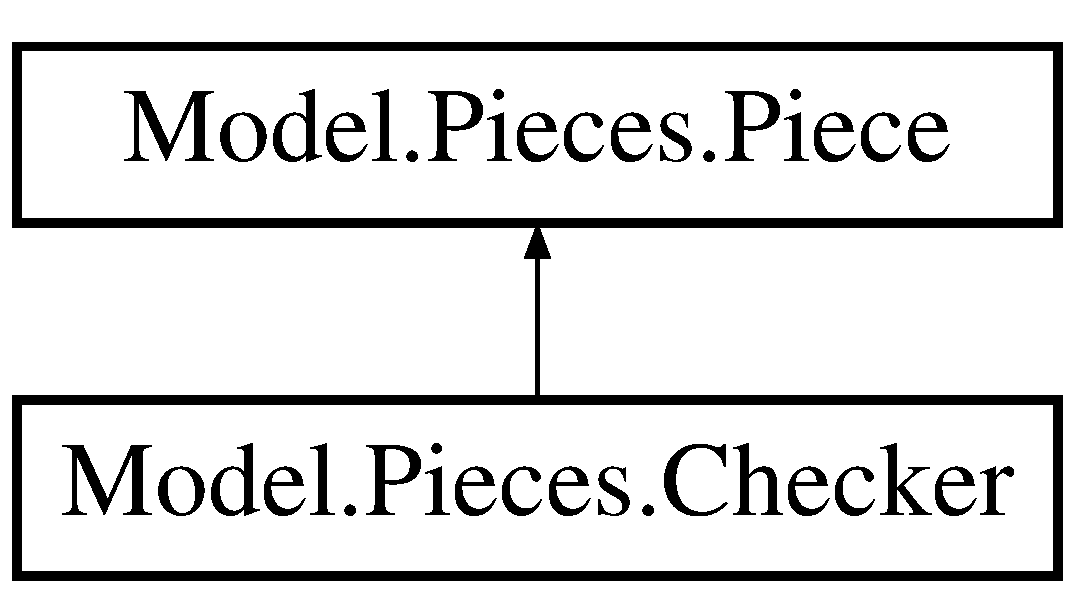
\includegraphics[height=2.000000cm]{class_model_1_1_pieces_1_1_checker}
\end{center}
\end{figure}
\subsection*{Public Member Functions}
\begin{DoxyCompactItemize}
\item 
\hyperlink{class_model_1_1_pieces_1_1_checker_af2b456d3e6c3ceff5a641fac1928fd5a}{Checker} (\hyperlink{class_model_1_1_team}{Team} team, int x\+Value, int y\+Value)
\item 
boolean \hyperlink{class_model_1_1_pieces_1_1_checker_a833ad4dc58dc068f194b30c5eb989d52}{is\+Valid\+Move} (\hyperlink{class_model_1_1_move}{Move} move, \hyperlink{class_model_1_1_board}{Board} board)
\item 
boolean \hyperlink{class_model_1_1_pieces_1_1_checker_ada084337407a5dc86bee162d61de44a8}{check\+No\+Piece\+At\+Destination} (\hyperlink{class_model_1_1_move}{Move} move, \hyperlink{class_model_1_1_board}{Board} board)
\item 
boolean \hyperlink{class_model_1_1_pieces_1_1_checker_a493190714612bdc8125c475b41434c75}{has\+No\+Piece\+In\+Movement\+Route} (\hyperlink{class_model_1_1_move}{Move} move, \hyperlink{class_model_1_1_board}{Board} board)
\item 
List$<$ \hyperlink{class_model_1_1_move}{Move} $>$ \hyperlink{class_model_1_1_pieces_1_1_checker_a840159766272906e7d72551c92623eee}{find\+All\+Moves} (\hyperlink{class_model_1_1_board}{Board} board)
\end{DoxyCompactItemize}


\subsection{Detailed Description}
\hyperlink{class_model_1_1_pieces_1_1_pawn}{Pawn} class to describe \hyperlink{class_model_1_1_pieces_1_1_checker}{Checker}\textquotesingle{}s possible moves. A \hyperlink{class_model_1_1_pieces_1_1_checker}{Checker} can move 1 space diagonally in any direction or if there is a piece diagonally adjacent to it, it can jump over that piece, thus moving 2 diagonally (similar to a \hyperlink{class_model_1_1_pieces_1_1_checker}{Checker} would in the game Checkers) \begin{DoxyAuthor}{Author}
arnavmishra 
\end{DoxyAuthor}


\subsection{Constructor \& Destructor Documentation}
\hypertarget{class_model_1_1_pieces_1_1_checker_af2b456d3e6c3ceff5a641fac1928fd5a}{}\label{class_model_1_1_pieces_1_1_checker_af2b456d3e6c3ceff5a641fac1928fd5a} 
\index{Model\+::\+Pieces\+::\+Checker@{Model\+::\+Pieces\+::\+Checker}!Checker@{Checker}}
\index{Checker@{Checker}!Model\+::\+Pieces\+::\+Checker@{Model\+::\+Pieces\+::\+Checker}}
\subsubsection{\texorpdfstring{Checker()}{Checker()}}
{\footnotesize\ttfamily Model.\+Pieces.\+Checker.\+Checker (\begin{DoxyParamCaption}\item[{\hyperlink{class_model_1_1_team}{Team}}]{team,  }\item[{int}]{x\+Value,  }\item[{int}]{y\+Value }\end{DoxyParamCaption})}

Constructor to initialize \hyperlink{class_model_1_1_pieces_1_1_checker}{Checker} on a team and coordinate. 
\begin{DoxyParams}{Parameters}
{\em team} & \\
\hline
\end{DoxyParams}


\subsection{Member Function Documentation}
\hypertarget{class_model_1_1_pieces_1_1_checker_ada084337407a5dc86bee162d61de44a8}{}\label{class_model_1_1_pieces_1_1_checker_ada084337407a5dc86bee162d61de44a8} 
\index{Model\+::\+Pieces\+::\+Checker@{Model\+::\+Pieces\+::\+Checker}!check\+No\+Piece\+At\+Destination@{check\+No\+Piece\+At\+Destination}}
\index{check\+No\+Piece\+At\+Destination@{check\+No\+Piece\+At\+Destination}!Model\+::\+Pieces\+::\+Checker@{Model\+::\+Pieces\+::\+Checker}}
\subsubsection{\texorpdfstring{check\+No\+Piece\+At\+Destination()}{checkNoPieceAtDestination()}}
{\footnotesize\ttfamily boolean Model.\+Pieces.\+Checker.\+check\+No\+Piece\+At\+Destination (\begin{DoxyParamCaption}\item[{\hyperlink{class_model_1_1_move}{Move}}]{move,  }\item[{\hyperlink{class_model_1_1_board}{Board}}]{board }\end{DoxyParamCaption})}

Helper function to confirm that there is no piece where the checker is moving for forward movement. 
\begin{DoxyParams}{Parameters}
{\em move} & \\
\hline
{\em board} & \\
\hline
\end{DoxyParams}
\begin{DoxyReturn}{Returns}
whether there is already a piece at the destination 
\end{DoxyReturn}
\hypertarget{class_model_1_1_pieces_1_1_checker_a840159766272906e7d72551c92623eee}{}\label{class_model_1_1_pieces_1_1_checker_a840159766272906e7d72551c92623eee} 
\index{Model\+::\+Pieces\+::\+Checker@{Model\+::\+Pieces\+::\+Checker}!find\+All\+Moves@{find\+All\+Moves}}
\index{find\+All\+Moves@{find\+All\+Moves}!Model\+::\+Pieces\+::\+Checker@{Model\+::\+Pieces\+::\+Checker}}
\subsubsection{\texorpdfstring{find\+All\+Moves()}{findAllMoves()}}
{\footnotesize\ttfamily List$<$\hyperlink{class_model_1_1_move}{Move}$>$ Model.\+Pieces.\+Checker.\+find\+All\+Moves (\begin{DoxyParamCaption}\item[{\hyperlink{class_model_1_1_board}{Board}}]{board }\end{DoxyParamCaption})}

Function to get all valid possible moves for the \hyperlink{class_model_1_1_pieces_1_1_checker}{Checker} in any direction. 
\begin{DoxyParams}{Parameters}
{\em board} & \\
\hline
\end{DoxyParams}
\begin{DoxyReturn}{Returns}
all possible valid moves. 
\end{DoxyReturn}
\hypertarget{class_model_1_1_pieces_1_1_checker_a493190714612bdc8125c475b41434c75}{}\label{class_model_1_1_pieces_1_1_checker_a493190714612bdc8125c475b41434c75} 
\index{Model\+::\+Pieces\+::\+Checker@{Model\+::\+Pieces\+::\+Checker}!has\+No\+Piece\+In\+Movement\+Route@{has\+No\+Piece\+In\+Movement\+Route}}
\index{has\+No\+Piece\+In\+Movement\+Route@{has\+No\+Piece\+In\+Movement\+Route}!Model\+::\+Pieces\+::\+Checker@{Model\+::\+Pieces\+::\+Checker}}
\subsubsection{\texorpdfstring{has\+No\+Piece\+In\+Movement\+Route()}{hasNoPieceInMovementRoute()}}
{\footnotesize\ttfamily boolean Model.\+Pieces.\+Checker.\+has\+No\+Piece\+In\+Movement\+Route (\begin{DoxyParamCaption}\item[{\hyperlink{class_model_1_1_move}{Move}}]{move,  }\item[{\hyperlink{class_model_1_1_board}{Board}}]{board }\end{DoxyParamCaption})}

Check that the pawn doesn\textquotesingle{}t jump over any piece. 
\begin{DoxyParams}{Parameters}
{\em move} & \\
\hline
{\em board} & \\
\hline
\end{DoxyParams}
\begin{DoxyReturn}{Returns}
whether the pawn leaps over pieces. 
\end{DoxyReturn}
\hypertarget{class_model_1_1_pieces_1_1_checker_a833ad4dc58dc068f194b30c5eb989d52}{}\label{class_model_1_1_pieces_1_1_checker_a833ad4dc58dc068f194b30c5eb989d52} 
\index{Model\+::\+Pieces\+::\+Checker@{Model\+::\+Pieces\+::\+Checker}!is\+Valid\+Move@{is\+Valid\+Move}}
\index{is\+Valid\+Move@{is\+Valid\+Move}!Model\+::\+Pieces\+::\+Checker@{Model\+::\+Pieces\+::\+Checker}}
\subsubsection{\texorpdfstring{is\+Valid\+Move()}{isValidMove()}}
{\footnotesize\ttfamily boolean Model.\+Pieces.\+Checker.\+is\+Valid\+Move (\begin{DoxyParamCaption}\item[{\hyperlink{class_model_1_1_move}{Move}}]{move,  }\item[{\hyperlink{class_model_1_1_board}{Board}}]{board }\end{DoxyParamCaption})}

Function to check whether a checker\textquotesingle{}s move is valid. 
\begin{DoxyParams}{Parameters}
{\em move} & \\
\hline
{\em board} & \\
\hline
\end{DoxyParams}
\begin{DoxyReturn}{Returns}
Whether the move is valid. 
\end{DoxyReturn}


The documentation for this class was generated from the following file\+:\begin{DoxyCompactItemize}
\item 
src/\+Model/\+Pieces/Checker.\+java\end{DoxyCompactItemize}

\hypertarget{class_tests_1_1_checker_test}{}\section{Tests.\+Checker\+Test Class Reference}
\label{class_tests_1_1_checker_test}\index{Tests.\+Checker\+Test@{Tests.\+Checker\+Test}}
\subsection*{Public Member Functions}
\begin{DoxyCompactItemize}
\item 
void \hyperlink{class_tests_1_1_checker_test_a93db61a292d48963a5ab97e349c910c3}{valid\+Checker\+Movement} ()  throws Exception 
\item 
void \hyperlink{class_tests_1_1_checker_test_a35af29acb3ae72737413763ace0f911e}{valid\+Checker\+Leap\+Movement} ()  throws Exception 
\item 
void \hyperlink{class_tests_1_1_checker_test_ac9d201b3122764534da6751a881509ee}{invalid\+Checker\+Movement} ()  throws Exception 
\item 
void \hyperlink{class_tests_1_1_checker_test_abff00b6e6dc767071f07e864a4636a63}{invalid\+Checker\+Leap\+Movement} ()  throws Exception 
\item 
void \hyperlink{class_tests_1_1_checker_test_a5eff464f77823f680ce240ca305bbbd9}{correct\+All\+Checker\+Moves} ()  throws Exception 
\end{DoxyCompactItemize}


\subsection{Detailed Description}
Tests for the Checker Class. \begin{DoxyAuthor}{Author}
arnavmishra 
\end{DoxyAuthor}


\subsection{Member Function Documentation}
\hypertarget{class_tests_1_1_checker_test_a5eff464f77823f680ce240ca305bbbd9}{}\label{class_tests_1_1_checker_test_a5eff464f77823f680ce240ca305bbbd9} 
\index{Tests\+::\+Checker\+Test@{Tests\+::\+Checker\+Test}!correct\+All\+Checker\+Moves@{correct\+All\+Checker\+Moves}}
\index{correct\+All\+Checker\+Moves@{correct\+All\+Checker\+Moves}!Tests\+::\+Checker\+Test@{Tests\+::\+Checker\+Test}}
\subsubsection{\texorpdfstring{correct\+All\+Checker\+Moves()}{correctAllCheckerMoves()}}
{\footnotesize\ttfamily void Tests.\+Checker\+Test.\+correct\+All\+Checker\+Moves (\begin{DoxyParamCaption}{ }\end{DoxyParamCaption}) throws Exception}

Test to check the checker\textquotesingle{}s possible movements by testing to ensure that the checker can move to all diagonal positions. 
\begin{DoxyExceptions}{Exceptions}
{\em Exception} & \\
\hline
\end{DoxyExceptions}
\hypertarget{class_tests_1_1_checker_test_abff00b6e6dc767071f07e864a4636a63}{}\label{class_tests_1_1_checker_test_abff00b6e6dc767071f07e864a4636a63} 
\index{Tests\+::\+Checker\+Test@{Tests\+::\+Checker\+Test}!invalid\+Checker\+Leap\+Movement@{invalid\+Checker\+Leap\+Movement}}
\index{invalid\+Checker\+Leap\+Movement@{invalid\+Checker\+Leap\+Movement}!Tests\+::\+Checker\+Test@{Tests\+::\+Checker\+Test}}
\subsubsection{\texorpdfstring{invalid\+Checker\+Leap\+Movement()}{invalidCheckerLeapMovement()}}
{\footnotesize\ttfamily void Tests.\+Checker\+Test.\+invalid\+Checker\+Leap\+Movement (\begin{DoxyParamCaption}{ }\end{DoxyParamCaption}) throws Exception}

Test to check checker\textquotesingle{}s invalid leap movement by trying to jump it over another piece into a non-\/vacant square. 
\begin{DoxyExceptions}{Exceptions}
{\em Exception} & \\
\hline
\end{DoxyExceptions}
\hypertarget{class_tests_1_1_checker_test_ac9d201b3122764534da6751a881509ee}{}\label{class_tests_1_1_checker_test_ac9d201b3122764534da6751a881509ee} 
\index{Tests\+::\+Checker\+Test@{Tests\+::\+Checker\+Test}!invalid\+Checker\+Movement@{invalid\+Checker\+Movement}}
\index{invalid\+Checker\+Movement@{invalid\+Checker\+Movement}!Tests\+::\+Checker\+Test@{Tests\+::\+Checker\+Test}}
\subsubsection{\texorpdfstring{invalid\+Checker\+Movement()}{invalidCheckerMovement()}}
{\footnotesize\ttfamily void Tests.\+Checker\+Test.\+invalid\+Checker\+Movement (\begin{DoxyParamCaption}{ }\end{DoxyParamCaption}) throws Exception}

Test to check checker\textquotesingle{}s invalid movement by trying to move it two spaces instead of a single space. 
\begin{DoxyExceptions}{Exceptions}
{\em Exception} & \\
\hline
\end{DoxyExceptions}
\hypertarget{class_tests_1_1_checker_test_a35af29acb3ae72737413763ace0f911e}{}\label{class_tests_1_1_checker_test_a35af29acb3ae72737413763ace0f911e} 
\index{Tests\+::\+Checker\+Test@{Tests\+::\+Checker\+Test}!valid\+Checker\+Leap\+Movement@{valid\+Checker\+Leap\+Movement}}
\index{valid\+Checker\+Leap\+Movement@{valid\+Checker\+Leap\+Movement}!Tests\+::\+Checker\+Test@{Tests\+::\+Checker\+Test}}
\subsubsection{\texorpdfstring{valid\+Checker\+Leap\+Movement()}{validCheckerLeapMovement()}}
{\footnotesize\ttfamily void Tests.\+Checker\+Test.\+valid\+Checker\+Leap\+Movement (\begin{DoxyParamCaption}{ }\end{DoxyParamCaption}) throws Exception}

Test to check the checker\textquotesingle{}s valid leap movement by placing the checker on the board and trying to move it diagonally. 
\begin{DoxyExceptions}{Exceptions}
{\em Exception} & \\
\hline
\end{DoxyExceptions}
\hypertarget{class_tests_1_1_checker_test_a93db61a292d48963a5ab97e349c910c3}{}\label{class_tests_1_1_checker_test_a93db61a292d48963a5ab97e349c910c3} 
\index{Tests\+::\+Checker\+Test@{Tests\+::\+Checker\+Test}!valid\+Checker\+Movement@{valid\+Checker\+Movement}}
\index{valid\+Checker\+Movement@{valid\+Checker\+Movement}!Tests\+::\+Checker\+Test@{Tests\+::\+Checker\+Test}}
\subsubsection{\texorpdfstring{valid\+Checker\+Movement()}{validCheckerMovement()}}
{\footnotesize\ttfamily void Tests.\+Checker\+Test.\+valid\+Checker\+Movement (\begin{DoxyParamCaption}{ }\end{DoxyParamCaption}) throws Exception}

Test to check the checker\textquotesingle{}s valid movement by placing the checker on the board and trying to move it diagonally. 
\begin{DoxyExceptions}{Exceptions}
{\em Exception} & \\
\hline
\end{DoxyExceptions}


The documentation for this class was generated from the following file\+:\begin{DoxyCompactItemize}
\item 
src/\+Tests/Checker\+Test.\+java\end{DoxyCompactItemize}

\hypertarget{class_tests_1_1_common}{}\section{Tests.\+Common Class Reference}
\label{class_tests_1_1_common}\index{Tests.\+Common@{Tests.\+Common}}
\subsection*{Static Public Member Functions}
\begin{DoxyCompactItemize}
\item 
static boolean \hyperlink{class_tests_1_1_common_a88d6dce17bfea9b706c866e0c896715d}{check\+If\+Move\+Lists\+Are\+Equal} (List$<$ \hyperlink{class_framework_1_1_move}{Move} $>$ expected, List$<$ \hyperlink{class_framework_1_1_move}{Move} $>$ actual)
\item 
static void \hyperlink{class_tests_1_1_common_a5809bd3c5d93653260370e00f74aad6a}{move\+Piece} (\hyperlink{class_framework_1_1_board}{Board} board, int startX, int startY, int endX, int endY, int team\+Number)
\end{DoxyCompactItemize}


\subsection{Detailed Description}
\hyperlink{class_tests_1_1_common}{Common} class to hold any common methods across the tests. \begin{DoxyAuthor}{Author}
arnavmishra 
\end{DoxyAuthor}


\subsection{Member Function Documentation}
\hypertarget{class_tests_1_1_common_a88d6dce17bfea9b706c866e0c896715d}{}\label{class_tests_1_1_common_a88d6dce17bfea9b706c866e0c896715d} 
\index{Tests\+::\+Common@{Tests\+::\+Common}!check\+If\+Move\+Lists\+Are\+Equal@{check\+If\+Move\+Lists\+Are\+Equal}}
\index{check\+If\+Move\+Lists\+Are\+Equal@{check\+If\+Move\+Lists\+Are\+Equal}!Tests\+::\+Common@{Tests\+::\+Common}}
\subsubsection{\texorpdfstring{check\+If\+Move\+Lists\+Are\+Equal()}{checkIfMoveListsAreEqual()}}
{\footnotesize\ttfamily static boolean Tests.\+Common.\+check\+If\+Move\+Lists\+Are\+Equal (\begin{DoxyParamCaption}\item[{List$<$ \hyperlink{class_framework_1_1_move}{Move} $>$}]{expected,  }\item[{List$<$ \hyperlink{class_framework_1_1_move}{Move} $>$}]{actual }\end{DoxyParamCaption})\hspace{0.3cm}{\ttfamily [static]}}

Helper method to check if two lists of moves are the same by checking that every move has the same start and end coordinates and team number. This is used to confirm that the lists of all possible moves in each piece class is correct. 
\begin{DoxyParams}{Parameters}
{\em expected} & \\
\hline
{\em actual} & \\
\hline
\end{DoxyParams}
\begin{DoxyReturn}{Returns}
True/\+False whether the lists are equal. 
\end{DoxyReturn}
\hypertarget{class_tests_1_1_common_a5809bd3c5d93653260370e00f74aad6a}{}\label{class_tests_1_1_common_a5809bd3c5d93653260370e00f74aad6a} 
\index{Tests\+::\+Common@{Tests\+::\+Common}!move\+Piece@{move\+Piece}}
\index{move\+Piece@{move\+Piece}!Tests\+::\+Common@{Tests\+::\+Common}}
\subsubsection{\texorpdfstring{move\+Piece()}{movePiece()}}
{\footnotesize\ttfamily static void Tests.\+Common.\+move\+Piece (\begin{DoxyParamCaption}\item[{\hyperlink{class_framework_1_1_board}{Board}}]{board,  }\item[{int}]{startX,  }\item[{int}]{startY,  }\item[{int}]{endX,  }\item[{int}]{endY,  }\item[{int}]{team\+Number }\end{DoxyParamCaption})\hspace{0.3cm}{\ttfamily [static]}}

Helper Function to move coordinates on a board. 
\begin{DoxyParams}{Parameters}
{\em board} & \\
\hline
{\em startX} & \\
\hline
{\em startY} & \\
\hline
{\em endX} & \\
\hline
{\em endY} & \\
\hline
{\em team\+Number} & \\
\hline
\end{DoxyParams}


The documentation for this class was generated from the following file\+:\begin{DoxyCompactItemize}
\item 
src/\+Tests/\hyperlink{_common_8java}{Common.\+java}\end{DoxyCompactItemize}

\hypertarget{class_model_1_1_pieces_1_1_ferz}{}\section{Model.\+Pieces.\+Ferz Class Reference}
\label{class_model_1_1_pieces_1_1_ferz}\index{Model.\+Pieces.\+Ferz@{Model.\+Pieces.\+Ferz}}
Inheritance diagram for Model.\+Pieces.\+Ferz\+:\begin{figure}[H]
\begin{center}
\leavevmode
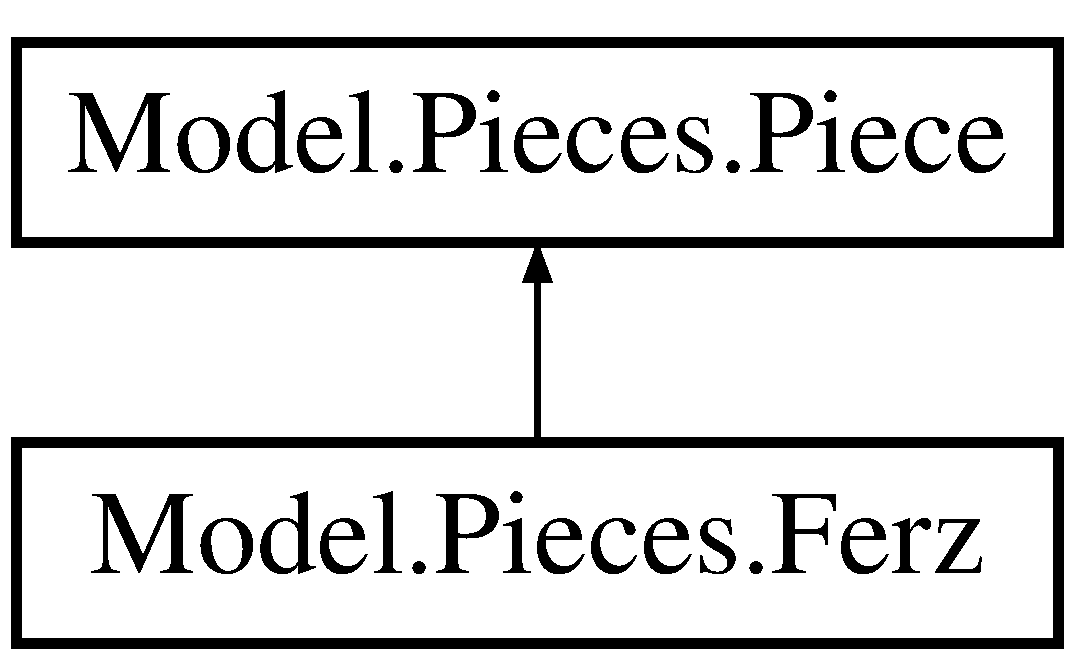
\includegraphics[height=2.000000cm]{class_model_1_1_pieces_1_1_ferz}
\end{center}
\end{figure}
\subsection*{Public Member Functions}
\begin{DoxyCompactItemize}
\item 
\hyperlink{class_model_1_1_pieces_1_1_ferz_a67c4619c704f514b56bfee13b922ef7b}{Ferz} (\hyperlink{class_model_1_1_team}{Team} team, int x\+Value, int y\+Value)
\item 
boolean \hyperlink{class_model_1_1_pieces_1_1_ferz_a0251ed6241fd3884b7f192659f44a9bd}{is\+Valid\+Move} (\hyperlink{class_model_1_1_move}{Move} move, \hyperlink{class_model_1_1_board}{Board} board)
\item 
boolean \hyperlink{class_model_1_1_pieces_1_1_ferz_a71d7e41b8171d621ce3f2f83791fbdc5}{has\+No\+Piece\+In\+Movement\+Route} (\hyperlink{class_model_1_1_move}{Move} move, \hyperlink{class_model_1_1_board}{Board} board)
\item 
List$<$ \hyperlink{class_model_1_1_move}{Move} $>$ \hyperlink{class_model_1_1_pieces_1_1_ferz_a86f35019ec569ae71b9c1d8a3e390df8}{find\+All\+Moves} (\hyperlink{class_model_1_1_board}{Board} board)
\item 
List$<$ \hyperlink{class_model_1_1_move}{Move} $>$ \hyperlink{class_model_1_1_pieces_1_1_ferz_a8359fecbb4158e2e00efcd1561e86177}{add\+Move\+To\+Possible\+Moves} (\hyperlink{class_model_1_1_board}{Board} board, int x\+Value, int y\+Value, int x\+Diff, int y\+Diff, List$<$ \hyperlink{class_model_1_1_move}{Move} $>$ possible\+Moves)
\end{DoxyCompactItemize}


\subsection{Detailed Description}
\hyperlink{class_model_1_1_pieces_1_1_ferz}{Ferz} class to describe \hyperlink{class_model_1_1_pieces_1_1_ferz}{Ferz}\textquotesingle{}s possible moves. \begin{DoxyAuthor}{Author}
arnavmishra 
\end{DoxyAuthor}


\subsection{Constructor \& Destructor Documentation}
\hypertarget{class_model_1_1_pieces_1_1_ferz_a67c4619c704f514b56bfee13b922ef7b}{}\label{class_model_1_1_pieces_1_1_ferz_a67c4619c704f514b56bfee13b922ef7b} 
\index{Model\+::\+Pieces\+::\+Ferz@{Model\+::\+Pieces\+::\+Ferz}!Ferz@{Ferz}}
\index{Ferz@{Ferz}!Model\+::\+Pieces\+::\+Ferz@{Model\+::\+Pieces\+::\+Ferz}}
\subsubsection{\texorpdfstring{Ferz()}{Ferz()}}
{\footnotesize\ttfamily Model.\+Pieces.\+Ferz.\+Ferz (\begin{DoxyParamCaption}\item[{\hyperlink{class_model_1_1_team}{Team}}]{team,  }\item[{int}]{x\+Value,  }\item[{int}]{y\+Value }\end{DoxyParamCaption})}

Constructor to initialize \hyperlink{class_model_1_1_pieces_1_1_ferz}{Ferz} on a team and coordinate. 
\begin{DoxyParams}{Parameters}
{\em team} & \\
\hline
\end{DoxyParams}


\subsection{Member Function Documentation}
\hypertarget{class_model_1_1_pieces_1_1_ferz_a8359fecbb4158e2e00efcd1561e86177}{}\label{class_model_1_1_pieces_1_1_ferz_a8359fecbb4158e2e00efcd1561e86177} 
\index{Model\+::\+Pieces\+::\+Ferz@{Model\+::\+Pieces\+::\+Ferz}!add\+Move\+To\+Possible\+Moves@{add\+Move\+To\+Possible\+Moves}}
\index{add\+Move\+To\+Possible\+Moves@{add\+Move\+To\+Possible\+Moves}!Model\+::\+Pieces\+::\+Ferz@{Model\+::\+Pieces\+::\+Ferz}}
\subsubsection{\texorpdfstring{add\+Move\+To\+Possible\+Moves()}{addMoveToPossibleMoves()}}
{\footnotesize\ttfamily List$<$\hyperlink{class_model_1_1_move}{Move}$>$ Model.\+Pieces.\+Ferz.\+add\+Move\+To\+Possible\+Moves (\begin{DoxyParamCaption}\item[{\hyperlink{class_model_1_1_board}{Board}}]{board,  }\item[{int}]{x\+Value,  }\item[{int}]{y\+Value,  }\item[{int}]{x\+Diff,  }\item[{int}]{y\+Diff,  }\item[{List$<$ \hyperlink{class_model_1_1_move}{Move} $>$}]{possible\+Moves }\end{DoxyParamCaption})}

Helper function to add a piece to the possible moves list after confirming validity 
\begin{DoxyParams}{Parameters}
{\em board} & \\
\hline
{\em x\+Value} & \\
\hline
{\em y\+Value} & \\
\hline
{\em x\+Diff} & \\
\hline
{\em y\+Diff} & \\
\hline
{\em possible\+Moves} & \\
\hline
\end{DoxyParams}
\begin{DoxyReturn}{Returns}
list with or without new move depending on whether it is possible 
\end{DoxyReturn}
\hypertarget{class_model_1_1_pieces_1_1_ferz_a86f35019ec569ae71b9c1d8a3e390df8}{}\label{class_model_1_1_pieces_1_1_ferz_a86f35019ec569ae71b9c1d8a3e390df8} 
\index{Model\+::\+Pieces\+::\+Ferz@{Model\+::\+Pieces\+::\+Ferz}!find\+All\+Moves@{find\+All\+Moves}}
\index{find\+All\+Moves@{find\+All\+Moves}!Model\+::\+Pieces\+::\+Ferz@{Model\+::\+Pieces\+::\+Ferz}}
\subsubsection{\texorpdfstring{find\+All\+Moves()}{findAllMoves()}}
{\footnotesize\ttfamily List$<$\hyperlink{class_model_1_1_move}{Move}$>$ Model.\+Pieces.\+Ferz.\+find\+All\+Moves (\begin{DoxyParamCaption}\item[{\hyperlink{class_model_1_1_board}{Board}}]{board }\end{DoxyParamCaption})}

Function to get all valid possible moves for the \hyperlink{class_model_1_1_pieces_1_1_ferz}{Ferz} in any direction. 
\begin{DoxyParams}{Parameters}
{\em board} & \\
\hline
\end{DoxyParams}
\begin{DoxyReturn}{Returns}
all possible valid moves. 
\end{DoxyReturn}
\hypertarget{class_model_1_1_pieces_1_1_ferz_a71d7e41b8171d621ce3f2f83791fbdc5}{}\label{class_model_1_1_pieces_1_1_ferz_a71d7e41b8171d621ce3f2f83791fbdc5} 
\index{Model\+::\+Pieces\+::\+Ferz@{Model\+::\+Pieces\+::\+Ferz}!has\+No\+Piece\+In\+Movement\+Route@{has\+No\+Piece\+In\+Movement\+Route}}
\index{has\+No\+Piece\+In\+Movement\+Route@{has\+No\+Piece\+In\+Movement\+Route}!Model\+::\+Pieces\+::\+Ferz@{Model\+::\+Pieces\+::\+Ferz}}
\subsubsection{\texorpdfstring{has\+No\+Piece\+In\+Movement\+Route()}{hasNoPieceInMovementRoute()}}
{\footnotesize\ttfamily boolean Model.\+Pieces.\+Ferz.\+has\+No\+Piece\+In\+Movement\+Route (\begin{DoxyParamCaption}\item[{\hyperlink{class_model_1_1_move}{Move}}]{move,  }\item[{\hyperlink{class_model_1_1_board}{Board}}]{board }\end{DoxyParamCaption})}

The ferz can\textquotesingle{}t jump over any pieces since it only moves one space. 
\begin{DoxyParams}{Parameters}
{\em move} & \\
\hline
{\em board} & \\
\hline
\end{DoxyParams}
\begin{DoxyReturn}{Returns}
whether the ferz leaps over pieces. 
\end{DoxyReturn}
\hypertarget{class_model_1_1_pieces_1_1_ferz_a0251ed6241fd3884b7f192659f44a9bd}{}\label{class_model_1_1_pieces_1_1_ferz_a0251ed6241fd3884b7f192659f44a9bd} 
\index{Model\+::\+Pieces\+::\+Ferz@{Model\+::\+Pieces\+::\+Ferz}!is\+Valid\+Move@{is\+Valid\+Move}}
\index{is\+Valid\+Move@{is\+Valid\+Move}!Model\+::\+Pieces\+::\+Ferz@{Model\+::\+Pieces\+::\+Ferz}}
\subsubsection{\texorpdfstring{is\+Valid\+Move()}{isValidMove()}}
{\footnotesize\ttfamily boolean Model.\+Pieces.\+Ferz.\+is\+Valid\+Move (\begin{DoxyParamCaption}\item[{\hyperlink{class_model_1_1_move}{Move}}]{move,  }\item[{\hyperlink{class_model_1_1_board}{Board}}]{board }\end{DoxyParamCaption})}

Function to check whether a ferz\textquotesingle{}s move is valid. 
\begin{DoxyParams}{Parameters}
{\em move} & \\
\hline
{\em board} & \\
\hline
\end{DoxyParams}
\begin{DoxyReturn}{Returns}
Whether the move is valid. 
\end{DoxyReturn}


The documentation for this class was generated from the following file\+:\begin{DoxyCompactItemize}
\item 
src/\+Model/\+Pieces/Ferz.\+java\end{DoxyCompactItemize}

\hypertarget{class_tests_1_1_ferz_test}{}\section{Tests.\+Ferz\+Test Class Reference}
\label{class_tests_1_1_ferz_test}\index{Tests.\+Ferz\+Test@{Tests.\+Ferz\+Test}}
\subsection*{Public Member Functions}
\begin{DoxyCompactItemize}
\item 
void \hyperlink{class_tests_1_1_ferz_test_ab8577a15a8d3c03a84c2af880bf86d13}{valid\+Ferz\+Movement} ()  throws Exception 
\item 
void \hyperlink{class_tests_1_1_ferz_test_af69b9c0b5ea3735d6105c1025ad4f305}{invalid\+Ferz\+Movement} ()  throws Exception 
\item 
void \hyperlink{class_tests_1_1_ferz_test_a53d5f9199ad96f294b601cb1921b6231}{correct\+All\+Ferz\+Moves} ()  throws Exception 
\end{DoxyCompactItemize}


\subsection{Detailed Description}
Tests for the Ferz Class. \begin{DoxyAuthor}{Author}
arnavmishra 
\end{DoxyAuthor}


\subsection{Member Function Documentation}
\hypertarget{class_tests_1_1_ferz_test_a53d5f9199ad96f294b601cb1921b6231}{}\label{class_tests_1_1_ferz_test_a53d5f9199ad96f294b601cb1921b6231} 
\index{Tests\+::\+Ferz\+Test@{Tests\+::\+Ferz\+Test}!correct\+All\+Ferz\+Moves@{correct\+All\+Ferz\+Moves}}
\index{correct\+All\+Ferz\+Moves@{correct\+All\+Ferz\+Moves}!Tests\+::\+Ferz\+Test@{Tests\+::\+Ferz\+Test}}
\subsubsection{\texorpdfstring{correct\+All\+Ferz\+Moves()}{correctAllFerzMoves()}}
{\footnotesize\ttfamily void Tests.\+Ferz\+Test.\+correct\+All\+Ferz\+Moves (\begin{DoxyParamCaption}{ }\end{DoxyParamCaption}) throws Exception}

Test to check the ferz\textquotesingle{}s possible movements by testing to ensure that the ferz can move to all diagonal positions. 
\begin{DoxyExceptions}{Exceptions}
{\em Exception} & \\
\hline
\end{DoxyExceptions}
\hypertarget{class_tests_1_1_ferz_test_af69b9c0b5ea3735d6105c1025ad4f305}{}\label{class_tests_1_1_ferz_test_af69b9c0b5ea3735d6105c1025ad4f305} 
\index{Tests\+::\+Ferz\+Test@{Tests\+::\+Ferz\+Test}!invalid\+Ferz\+Movement@{invalid\+Ferz\+Movement}}
\index{invalid\+Ferz\+Movement@{invalid\+Ferz\+Movement}!Tests\+::\+Ferz\+Test@{Tests\+::\+Ferz\+Test}}
\subsubsection{\texorpdfstring{invalid\+Ferz\+Movement()}{invalidFerzMovement()}}
{\footnotesize\ttfamily void Tests.\+Ferz\+Test.\+invalid\+Ferz\+Movement (\begin{DoxyParamCaption}{ }\end{DoxyParamCaption}) throws Exception}

Test to check ferz\textquotesingle{}s invalid movement by trying to move it two spaces instead of a single space. 
\begin{DoxyExceptions}{Exceptions}
{\em Exception} & \\
\hline
\end{DoxyExceptions}
\hypertarget{class_tests_1_1_ferz_test_ab8577a15a8d3c03a84c2af880bf86d13}{}\label{class_tests_1_1_ferz_test_ab8577a15a8d3c03a84c2af880bf86d13} 
\index{Tests\+::\+Ferz\+Test@{Tests\+::\+Ferz\+Test}!valid\+Ferz\+Movement@{valid\+Ferz\+Movement}}
\index{valid\+Ferz\+Movement@{valid\+Ferz\+Movement}!Tests\+::\+Ferz\+Test@{Tests\+::\+Ferz\+Test}}
\subsubsection{\texorpdfstring{valid\+Ferz\+Movement()}{validFerzMovement()}}
{\footnotesize\ttfamily void Tests.\+Ferz\+Test.\+valid\+Ferz\+Movement (\begin{DoxyParamCaption}{ }\end{DoxyParamCaption}) throws Exception}

Test to check the ferz\textquotesingle{}s valid movement by placing the ferz on the board and trying to move it diagonally. 
\begin{DoxyExceptions}{Exceptions}
{\em Exception} & \\
\hline
\end{DoxyExceptions}


The documentation for this class was generated from the following file\+:\begin{DoxyCompactItemize}
\item 
src/\+Tests/Ferz\+Test.\+java\end{DoxyCompactItemize}

\hypertarget{class_controller_1_1_game}{}\section{Controller.\+Game Class Reference}
\label{class_controller_1_1_game}\index{Controller.\+Game@{Controller.\+Game}}
\subsection*{Static Public Member Functions}
\begin{DoxyCompactItemize}
\item 
static void \hyperlink{class_controller_1_1_game_a4835bc44e3401e01fe5ced7dba4b7524}{main} (String args\mbox{[}$\,$\mbox{]})
\item 
static int \hyperlink{class_controller_1_1_game_a805721bee4d26c4809276e9a0730cbee}{play\+Move} (\hyperlink{class_model_1_1_board}{Board} board, \hyperlink{class_model_1_1_pieces_1_1_piece}{Piece}\mbox{[}$\,$\mbox{]}\mbox{[}$\,$\mbox{]} positions, Scanner read\+Input, int turn\+Team\+Number)
\item 
static int \mbox{[}$\,$\mbox{]} \hyperlink{class_controller_1_1_game_acf1b89d047ccfd6b01e18e282cf091de}{get\+Inputs} (Scanner read\+Input)
\item 
static int \hyperlink{class_controller_1_1_game_ad1cc7d205bef9e3a36f071c8e158156c}{prompt\+For\+Undo\+Move} (\hyperlink{class_model_1_1_board}{Board} board, \hyperlink{class_model_1_1_pieces_1_1_piece}{Piece} removed\+Piece, \hyperlink{class_model_1_1_move}{Move} undo\+Move, Scanner read\+Input, int turn\+Team\+Number)
\end{DoxyCompactItemize}


\subsection{Detailed Description}
The \hyperlink{class_controller_1_1_game}{Game} class runs the primary game including developing the UI. \begin{DoxyAuthor}{Author}
arnavmishra Fastest check mate\+: 5153, 4645, 6163, 3773 
\end{DoxyAuthor}


\subsection{Member Function Documentation}
\hypertarget{class_controller_1_1_game_acf1b89d047ccfd6b01e18e282cf091de}{}\label{class_controller_1_1_game_acf1b89d047ccfd6b01e18e282cf091de} 
\index{Controller\+::\+Game@{Controller\+::\+Game}!get\+Inputs@{get\+Inputs}}
\index{get\+Inputs@{get\+Inputs}!Controller\+::\+Game@{Controller\+::\+Game}}
\subsubsection{\texorpdfstring{get\+Inputs()}{getInputs()}}
{\footnotesize\ttfamily static int \mbox{[}$\,$\mbox{]} Controller.\+Game.\+get\+Inputs (\begin{DoxyParamCaption}\item[{Scanner}]{read\+Input }\end{DoxyParamCaption})\hspace{0.3cm}{\ttfamily [static]}}

Helper function to get the input start and end coordinates for a move. 
\begin{DoxyParams}{Parameters}
{\em read\+Input} & \\
\hline
\end{DoxyParams}
\begin{DoxyReturn}{Returns}
the input values for the move. 
\end{DoxyReturn}
\hypertarget{class_controller_1_1_game_a4835bc44e3401e01fe5ced7dba4b7524}{}\label{class_controller_1_1_game_a4835bc44e3401e01fe5ced7dba4b7524} 
\index{Controller\+::\+Game@{Controller\+::\+Game}!main@{main}}
\index{main@{main}!Controller\+::\+Game@{Controller\+::\+Game}}
\subsubsection{\texorpdfstring{main()}{main()}}
{\footnotesize\ttfamily static void Controller.\+Game.\+main (\begin{DoxyParamCaption}\item[{String}]{args\mbox{[}$\,$\mbox{]} }\end{DoxyParamCaption})\hspace{0.3cm}{\ttfamily [static]}}

Main function to set-\/up the game and then start the moves. 
\begin{DoxyParams}{Parameters}
{\em args} & \\
\hline
\end{DoxyParams}
\hypertarget{class_controller_1_1_game_a805721bee4d26c4809276e9a0730cbee}{}\label{class_controller_1_1_game_a805721bee4d26c4809276e9a0730cbee} 
\index{Controller\+::\+Game@{Controller\+::\+Game}!play\+Move@{play\+Move}}
\index{play\+Move@{play\+Move}!Controller\+::\+Game@{Controller\+::\+Game}}
\subsubsection{\texorpdfstring{play\+Move()}{playMove()}}
{\footnotesize\ttfamily static int Controller.\+Game.\+play\+Move (\begin{DoxyParamCaption}\item[{\hyperlink{class_model_1_1_board}{Board}}]{board,  }\item[{\hyperlink{class_model_1_1_pieces_1_1_piece}{Piece}}]{positions\mbox{[}$\,$\mbox{]}\mbox{[}$\,$\mbox{]},  }\item[{Scanner}]{read\+Input,  }\item[{int}]{turn\+Team\+Number }\end{DoxyParamCaption})\hspace{0.3cm}{\ttfamily [static]}}

Method to run each move including checking for check, checkmate, stalemate, and validity of move. 
\begin{DoxyParams}{Parameters}
{\em board} & \\
\hline
{\em positions} & \\
\hline
{\em read\+Input} & \\
\hline
{\em turn\+Team\+Number} & \\
\hline
\end{DoxyParams}
\begin{DoxyReturn}{Returns}
which team\textquotesingle{}s turn it is. -\/1 when the game is done. 
\end{DoxyReturn}
\hypertarget{class_controller_1_1_game_ad1cc7d205bef9e3a36f071c8e158156c}{}\label{class_controller_1_1_game_ad1cc7d205bef9e3a36f071c8e158156c} 
\index{Controller\+::\+Game@{Controller\+::\+Game}!prompt\+For\+Undo\+Move@{prompt\+For\+Undo\+Move}}
\index{prompt\+For\+Undo\+Move@{prompt\+For\+Undo\+Move}!Controller\+::\+Game@{Controller\+::\+Game}}
\subsubsection{\texorpdfstring{prompt\+For\+Undo\+Move()}{promptForUndoMove()}}
{\footnotesize\ttfamily static int Controller.\+Game.\+prompt\+For\+Undo\+Move (\begin{DoxyParamCaption}\item[{\hyperlink{class_model_1_1_board}{Board}}]{board,  }\item[{\hyperlink{class_model_1_1_pieces_1_1_piece}{Piece}}]{removed\+Piece,  }\item[{\hyperlink{class_model_1_1_move}{Move}}]{undo\+Move,  }\item[{Scanner}]{read\+Input,  }\item[{int}]{turn\+Team\+Number }\end{DoxyParamCaption})\hspace{0.3cm}{\ttfamily [static]}}

Helper function to undo a move that a player makes. 
\begin{DoxyParams}{Parameters}
{\em board} & \\
\hline
{\em removed\+Piece} & \\
\hline
{\em undo\+Move} & \\
\hline
{\em read\+Input} & \\
\hline
{\em turn\+Team\+Number} & \\
\hline
\end{DoxyParams}
\begin{DoxyReturn}{Returns}
the Team\+Number for who\textquotesingle{}s turn it currently is. 
\end{DoxyReturn}


The documentation for this class was generated from the following file\+:\begin{DoxyCompactItemize}
\item 
src/\+Controller/Game.\+java\end{DoxyCompactItemize}

\hypertarget{class_view_1_1_g_u_i}{}\section{View.\+G\+UI Class Reference}
\label{class_view_1_1_g_u_i}\index{View.\+G\+UI@{View.\+G\+UI}}
\subsection*{Public Member Functions}
\begin{DoxyCompactItemize}
\item 
\hyperlink{class_view_1_1_g_u_i_a7a4bdade50043a2fc96ff3e7a6c13da8}{G\+UI} (\hyperlink{class_model_1_1_pieces_1_1_piece}{Piece}\mbox{[}$\,$\mbox{]}\mbox{[}$\,$\mbox{]} piece\+Positions)
\end{DoxyCompactItemize}
\subsection*{Static Public Member Functions}
\begin{DoxyCompactItemize}
\item 
static void \hyperlink{class_view_1_1_g_u_i_ab66997d351c41f53de8f3ee0ba838748}{main} (String\mbox{[}$\,$\mbox{]} args)
\end{DoxyCompactItemize}


\subsection{Detailed Description}
Sources\+: \href{http://stackoverflow.com/questions/299495/how-to-add-an-image-to-a-jpanel}{\tt http\+://stackoverflow.\+com/questions/299495/how-\/to-\/add-\/an-\/image-\/to-\/a-\/jpanel} \href{https://wiki.illinois.edu/wiki/pages/viewpage.action?spaceKey=cs242&title=Assignment+1.1}{\tt https\+://wiki.\+illinois.\+edu/wiki/pages/viewpage.\+action?space\+Key=cs242\&title=\+Assignment+1.\+1} \hyperlink{class_view_1_1_g_u_i}{G\+UI} class to develop primary chess board. \begin{DoxyAuthor}{Author}
arnavmishra 
\end{DoxyAuthor}


\subsection{Constructor \& Destructor Documentation}
\hypertarget{class_view_1_1_g_u_i_a7a4bdade50043a2fc96ff3e7a6c13da8}{}\label{class_view_1_1_g_u_i_a7a4bdade50043a2fc96ff3e7a6c13da8} 
\index{View\+::\+G\+UI@{View\+::\+G\+UI}!G\+UI@{G\+UI}}
\index{G\+UI@{G\+UI}!View\+::\+G\+UI@{View\+::\+G\+UI}}
\subsubsection{\texorpdfstring{G\+U\+I()}{GUI()}}
{\footnotesize\ttfamily View.\+G\+U\+I.\+G\+UI (\begin{DoxyParamCaption}\item[{\hyperlink{class_model_1_1_pieces_1_1_piece}{Piece}}]{piece\+Positions\mbox{[}$\,$\mbox{]}\mbox{[}$\,$\mbox{]} }\end{DoxyParamCaption})}

Constructor to create \hyperlink{class_view_1_1_g_u_i}{G\+UI} using positions of pieces on board. 
\begin{DoxyParams}{Parameters}
{\em piece\+Positions} & \\
\hline
\end{DoxyParams}


\subsection{Member Function Documentation}
\hypertarget{class_view_1_1_g_u_i_ab66997d351c41f53de8f3ee0ba838748}{}\label{class_view_1_1_g_u_i_ab66997d351c41f53de8f3ee0ba838748} 
\index{View\+::\+G\+UI@{View\+::\+G\+UI}!main@{main}}
\index{main@{main}!View\+::\+G\+UI@{View\+::\+G\+UI}}
\subsubsection{\texorpdfstring{main()}{main()}}
{\footnotesize\ttfamily static void View.\+G\+U\+I.\+main (\begin{DoxyParamCaption}\item[{String \mbox{[}$\,$\mbox{]}}]{args }\end{DoxyParamCaption})\hspace{0.3cm}{\ttfamily [static]}}

Main function to make initial board and to set up the \hyperlink{class_view_1_1_g_u_i}{G\+UI}. 
\begin{DoxyParams}{Parameters}
{\em args} & \\
\hline
\end{DoxyParams}


The documentation for this class was generated from the following file\+:\begin{DoxyCompactItemize}
\item 
src/\+View/G\+U\+I.\+java\end{DoxyCompactItemize}

\hypertarget{class_model_1_1_pieces_1_1_king}{}\section{Model.\+Pieces.\+King Class Reference}
\label{class_model_1_1_pieces_1_1_king}\index{Model.\+Pieces.\+King@{Model.\+Pieces.\+King}}
Inheritance diagram for Model.\+Pieces.\+King\+:\begin{figure}[H]
\begin{center}
\leavevmode
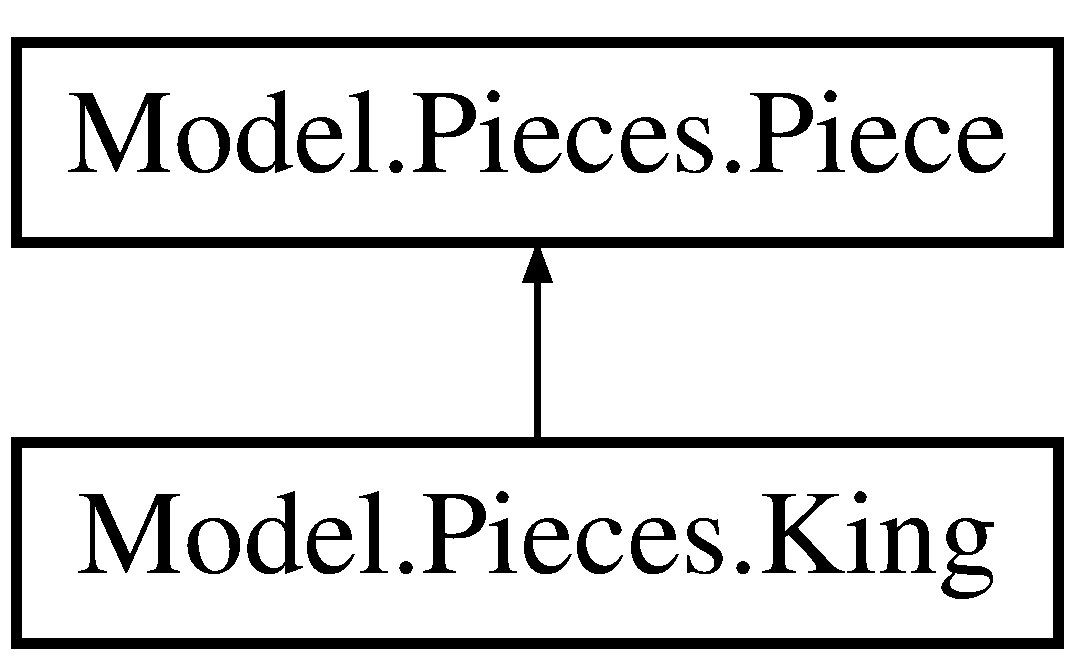
\includegraphics[height=2.000000cm]{class_model_1_1_pieces_1_1_king}
\end{center}
\end{figure}
\subsection*{Public Member Functions}
\begin{DoxyCompactItemize}
\item 
\hyperlink{class_model_1_1_pieces_1_1_king_a064e3c2161d2fc9153efb4618493550e}{King} (\hyperlink{class_model_1_1_team}{Team} team, int x\+Value, int y\+Value)
\item 
boolean \hyperlink{class_model_1_1_pieces_1_1_king_afdaa2fec4da9bc1c217e9a3c88700cea}{is\+Valid\+Move} (\hyperlink{class_model_1_1_move}{Move} move, \hyperlink{class_model_1_1_board}{Board} board)
\item 
boolean \hyperlink{class_model_1_1_pieces_1_1_king_aaf00b36ede859653e9c3ae8c72ea302c}{has\+No\+Piece\+In\+Movement\+Route} (\hyperlink{class_model_1_1_move}{Move} move, \hyperlink{class_model_1_1_board}{Board} board)
\item 
List$<$ \hyperlink{class_model_1_1_move}{Move} $>$ \hyperlink{class_model_1_1_pieces_1_1_king_ac947a57bac9d81d02b64e8bc470257bf}{find\+All\+Moves} (\hyperlink{class_model_1_1_board}{Board} board)
\item 
List$<$ \hyperlink{class_model_1_1_move}{Move} $>$ \hyperlink{class_model_1_1_pieces_1_1_king_a4d77bfe79a1c8087c8ce91397388c6d5}{add\+Move\+To\+Possible\+Moves} (\hyperlink{class_model_1_1_board}{Board} board, int x\+Value, int y\+Value, int x\+Diff, int y\+Diff, List$<$ \hyperlink{class_model_1_1_move}{Move} $>$ possible\+Moves)
\end{DoxyCompactItemize}


\subsection{Detailed Description}
\hyperlink{class_model_1_1_pieces_1_1_king}{King} class to describe \hyperlink{class_model_1_1_pieces_1_1_king}{King}\textquotesingle{}s possible moves. \begin{DoxyAuthor}{Author}
arnavmishra 
\end{DoxyAuthor}


\subsection{Constructor \& Destructor Documentation}
\hypertarget{class_model_1_1_pieces_1_1_king_a064e3c2161d2fc9153efb4618493550e}{}\label{class_model_1_1_pieces_1_1_king_a064e3c2161d2fc9153efb4618493550e} 
\index{Model\+::\+Pieces\+::\+King@{Model\+::\+Pieces\+::\+King}!King@{King}}
\index{King@{King}!Model\+::\+Pieces\+::\+King@{Model\+::\+Pieces\+::\+King}}
\subsubsection{\texorpdfstring{King()}{King()}}
{\footnotesize\ttfamily Model.\+Pieces.\+King.\+King (\begin{DoxyParamCaption}\item[{\hyperlink{class_model_1_1_team}{Team}}]{team,  }\item[{int}]{x\+Value,  }\item[{int}]{y\+Value }\end{DoxyParamCaption})}

Constructor to initialize \hyperlink{class_model_1_1_pieces_1_1_king}{King} on a team and coordinate. 
\begin{DoxyParams}{Parameters}
{\em team} & \\
\hline
\end{DoxyParams}


\subsection{Member Function Documentation}
\hypertarget{class_model_1_1_pieces_1_1_king_a4d77bfe79a1c8087c8ce91397388c6d5}{}\label{class_model_1_1_pieces_1_1_king_a4d77bfe79a1c8087c8ce91397388c6d5} 
\index{Model\+::\+Pieces\+::\+King@{Model\+::\+Pieces\+::\+King}!add\+Move\+To\+Possible\+Moves@{add\+Move\+To\+Possible\+Moves}}
\index{add\+Move\+To\+Possible\+Moves@{add\+Move\+To\+Possible\+Moves}!Model\+::\+Pieces\+::\+King@{Model\+::\+Pieces\+::\+King}}
\subsubsection{\texorpdfstring{add\+Move\+To\+Possible\+Moves()}{addMoveToPossibleMoves()}}
{\footnotesize\ttfamily List$<$\hyperlink{class_model_1_1_move}{Move}$>$ Model.\+Pieces.\+King.\+add\+Move\+To\+Possible\+Moves (\begin{DoxyParamCaption}\item[{\hyperlink{class_model_1_1_board}{Board}}]{board,  }\item[{int}]{x\+Value,  }\item[{int}]{y\+Value,  }\item[{int}]{x\+Diff,  }\item[{int}]{y\+Diff,  }\item[{List$<$ \hyperlink{class_model_1_1_move}{Move} $>$}]{possible\+Moves }\end{DoxyParamCaption})}

Helper function to add a piece to the possible moves list after confirming validity 
\begin{DoxyParams}{Parameters}
{\em board} & \\
\hline
{\em x\+Value} & \\
\hline
{\em y\+Value} & \\
\hline
{\em x\+Diff} & \\
\hline
{\em y\+Diff} & \\
\hline
{\em possible\+Moves} & \\
\hline
\end{DoxyParams}
\begin{DoxyReturn}{Returns}
list with or without new move depending on whether it is possible 
\end{DoxyReturn}
\hypertarget{class_model_1_1_pieces_1_1_king_ac947a57bac9d81d02b64e8bc470257bf}{}\label{class_model_1_1_pieces_1_1_king_ac947a57bac9d81d02b64e8bc470257bf} 
\index{Model\+::\+Pieces\+::\+King@{Model\+::\+Pieces\+::\+King}!find\+All\+Moves@{find\+All\+Moves}}
\index{find\+All\+Moves@{find\+All\+Moves}!Model\+::\+Pieces\+::\+King@{Model\+::\+Pieces\+::\+King}}
\subsubsection{\texorpdfstring{find\+All\+Moves()}{findAllMoves()}}
{\footnotesize\ttfamily List$<$\hyperlink{class_model_1_1_move}{Move}$>$ Model.\+Pieces.\+King.\+find\+All\+Moves (\begin{DoxyParamCaption}\item[{\hyperlink{class_model_1_1_board}{Board}}]{board }\end{DoxyParamCaption})}

Function to get all valid possible moves for the \hyperlink{class_model_1_1_pieces_1_1_king}{King} in any direction. 
\begin{DoxyParams}{Parameters}
{\em board} & \\
\hline
\end{DoxyParams}
\begin{DoxyReturn}{Returns}
all possible valid moves. 
\end{DoxyReturn}
\hypertarget{class_model_1_1_pieces_1_1_king_aaf00b36ede859653e9c3ae8c72ea302c}{}\label{class_model_1_1_pieces_1_1_king_aaf00b36ede859653e9c3ae8c72ea302c} 
\index{Model\+::\+Pieces\+::\+King@{Model\+::\+Pieces\+::\+King}!has\+No\+Piece\+In\+Movement\+Route@{has\+No\+Piece\+In\+Movement\+Route}}
\index{has\+No\+Piece\+In\+Movement\+Route@{has\+No\+Piece\+In\+Movement\+Route}!Model\+::\+Pieces\+::\+King@{Model\+::\+Pieces\+::\+King}}
\subsubsection{\texorpdfstring{has\+No\+Piece\+In\+Movement\+Route()}{hasNoPieceInMovementRoute()}}
{\footnotesize\ttfamily boolean Model.\+Pieces.\+King.\+has\+No\+Piece\+In\+Movement\+Route (\begin{DoxyParamCaption}\item[{\hyperlink{class_model_1_1_move}{Move}}]{move,  }\item[{\hyperlink{class_model_1_1_board}{Board}}]{board }\end{DoxyParamCaption})}

The king can\textquotesingle{}t jump over any pieces since it only moves one space. 
\begin{DoxyParams}{Parameters}
{\em move} & \\
\hline
{\em board} & \\
\hline
\end{DoxyParams}
\begin{DoxyReturn}{Returns}
whether the king leaps over pieces. 
\end{DoxyReturn}
\hypertarget{class_model_1_1_pieces_1_1_king_afdaa2fec4da9bc1c217e9a3c88700cea}{}\label{class_model_1_1_pieces_1_1_king_afdaa2fec4da9bc1c217e9a3c88700cea} 
\index{Model\+::\+Pieces\+::\+King@{Model\+::\+Pieces\+::\+King}!is\+Valid\+Move@{is\+Valid\+Move}}
\index{is\+Valid\+Move@{is\+Valid\+Move}!Model\+::\+Pieces\+::\+King@{Model\+::\+Pieces\+::\+King}}
\subsubsection{\texorpdfstring{is\+Valid\+Move()}{isValidMove()}}
{\footnotesize\ttfamily boolean Model.\+Pieces.\+King.\+is\+Valid\+Move (\begin{DoxyParamCaption}\item[{\hyperlink{class_model_1_1_move}{Move}}]{move,  }\item[{\hyperlink{class_model_1_1_board}{Board}}]{board }\end{DoxyParamCaption})}

Function to check whether a king\textquotesingle{}s move is valid. 
\begin{DoxyParams}{Parameters}
{\em move} & \\
\hline
{\em board} & \\
\hline
\end{DoxyParams}
\begin{DoxyReturn}{Returns}
Whether the move is valid. 
\end{DoxyReturn}


The documentation for this class was generated from the following file\+:\begin{DoxyCompactItemize}
\item 
src/\+Model/\+Pieces/King.\+java\end{DoxyCompactItemize}

\hypertarget{class_tests_1_1_king_test}{}\section{Tests.\+King\+Test Class Reference}
\label{class_tests_1_1_king_test}\index{Tests.\+King\+Test@{Tests.\+King\+Test}}
\subsection*{Public Member Functions}
\begin{DoxyCompactItemize}
\item 
void \hyperlink{class_tests_1_1_king_test_ae1c17c791c61a55e41358e79d65efb6a}{valid\+King\+Forward\+Movement} ()  throws Exception 
\item 
void \hyperlink{class_tests_1_1_king_test_a297113688dc835173504e520e6e1f8e5}{valid\+King\+Diagonal\+Movement} ()  throws Exception 
\item 
void \hyperlink{class_tests_1_1_king_test_a9f87b45c5ea04ab26343e828ffac02f6}{invalid\+King\+Movement} ()  throws Exception 
\item 
void \hyperlink{class_tests_1_1_king_test_a6ebd4a43cfa189c1f572ee5978d47330}{correct\+All\+Starting\+King\+Moves} ()  throws Exception 
\end{DoxyCompactItemize}


\subsection{Detailed Description}
\hyperlink{namespace_tests}{Tests} for the King class. \begin{DoxyAuthor}{Author}
arnavmishra 
\end{DoxyAuthor}


\subsection{Member Function Documentation}
\hypertarget{class_tests_1_1_king_test_a6ebd4a43cfa189c1f572ee5978d47330}{}\label{class_tests_1_1_king_test_a6ebd4a43cfa189c1f572ee5978d47330} 
\index{Tests\+::\+King\+Test@{Tests\+::\+King\+Test}!correct\+All\+Starting\+King\+Moves@{correct\+All\+Starting\+King\+Moves}}
\index{correct\+All\+Starting\+King\+Moves@{correct\+All\+Starting\+King\+Moves}!Tests\+::\+King\+Test@{Tests\+::\+King\+Test}}
\subsubsection{\texorpdfstring{correct\+All\+Starting\+King\+Moves()}{correctAllStartingKingMoves()}}
{\footnotesize\ttfamily void Tests.\+King\+Test.\+correct\+All\+Starting\+King\+Moves (\begin{DoxyParamCaption}{ }\end{DoxyParamCaption}) throws Exception}

Test to check the possible moves for the King by moving the pawn ahead and diagonal out of the way and ensuring the King can move to the open spots. 
\begin{DoxyExceptions}{Exceptions}
{\em Exception} & \\
\hline
\end{DoxyExceptions}
\hypertarget{class_tests_1_1_king_test_a9f87b45c5ea04ab26343e828ffac02f6}{}\label{class_tests_1_1_king_test_a9f87b45c5ea04ab26343e828ffac02f6} 
\index{Tests\+::\+King\+Test@{Tests\+::\+King\+Test}!invalid\+King\+Movement@{invalid\+King\+Movement}}
\index{invalid\+King\+Movement@{invalid\+King\+Movement}!Tests\+::\+King\+Test@{Tests\+::\+King\+Test}}
\subsubsection{\texorpdfstring{invalid\+King\+Movement()}{invalidKingMovement()}}
{\footnotesize\ttfamily void Tests.\+King\+Test.\+invalid\+King\+Movement (\begin{DoxyParamCaption}{ }\end{DoxyParamCaption}) throws Exception}

Test to check the King\textquotesingle{}s invalid movement by moving the King forward 2 spaces. 
\begin{DoxyExceptions}{Exceptions}
{\em Exception} & \\
\hline
\end{DoxyExceptions}
\hypertarget{class_tests_1_1_king_test_a297113688dc835173504e520e6e1f8e5}{}\label{class_tests_1_1_king_test_a297113688dc835173504e520e6e1f8e5} 
\index{Tests\+::\+King\+Test@{Tests\+::\+King\+Test}!valid\+King\+Diagonal\+Movement@{valid\+King\+Diagonal\+Movement}}
\index{valid\+King\+Diagonal\+Movement@{valid\+King\+Diagonal\+Movement}!Tests\+::\+King\+Test@{Tests\+::\+King\+Test}}
\subsubsection{\texorpdfstring{valid\+King\+Diagonal\+Movement()}{validKingDiagonalMovement()}}
{\footnotesize\ttfamily void Tests.\+King\+Test.\+valid\+King\+Diagonal\+Movement (\begin{DoxyParamCaption}{ }\end{DoxyParamCaption}) throws Exception}

Test to check the King\textquotesingle{}s diagonal movement by moving the pawn diagonally (left up) ahead out of the way and moving the King in that direction. 
\begin{DoxyExceptions}{Exceptions}
{\em Exception} & \\
\hline
\end{DoxyExceptions}
\hypertarget{class_tests_1_1_king_test_ae1c17c791c61a55e41358e79d65efb6a}{}\label{class_tests_1_1_king_test_ae1c17c791c61a55e41358e79d65efb6a} 
\index{Tests\+::\+King\+Test@{Tests\+::\+King\+Test}!valid\+King\+Forward\+Movement@{valid\+King\+Forward\+Movement}}
\index{valid\+King\+Forward\+Movement@{valid\+King\+Forward\+Movement}!Tests\+::\+King\+Test@{Tests\+::\+King\+Test}}
\subsubsection{\texorpdfstring{valid\+King\+Forward\+Movement()}{validKingForwardMovement()}}
{\footnotesize\ttfamily void Tests.\+King\+Test.\+valid\+King\+Forward\+Movement (\begin{DoxyParamCaption}{ }\end{DoxyParamCaption}) throws Exception}

Test to check the king\textquotesingle{}s forward movement by moving the pawn ahead of it out of the way and ensuring that the King can move forward. 
\begin{DoxyExceptions}{Exceptions}
{\em Exception} & \\
\hline
\end{DoxyExceptions}


The documentation for this class was generated from the following file\+:\begin{DoxyCompactItemize}
\item 
src/\+Tests/\hyperlink{_king_test_8java}{King\+Test.\+java}\end{DoxyCompactItemize}

\hypertarget{class_model_1_1_pieces_1_1_knight}{}\section{Model.\+Pieces.\+Knight Class Reference}
\label{class_model_1_1_pieces_1_1_knight}\index{Model.\+Pieces.\+Knight@{Model.\+Pieces.\+Knight}}
Inheritance diagram for Model.\+Pieces.\+Knight\+:\begin{figure}[H]
\begin{center}
\leavevmode
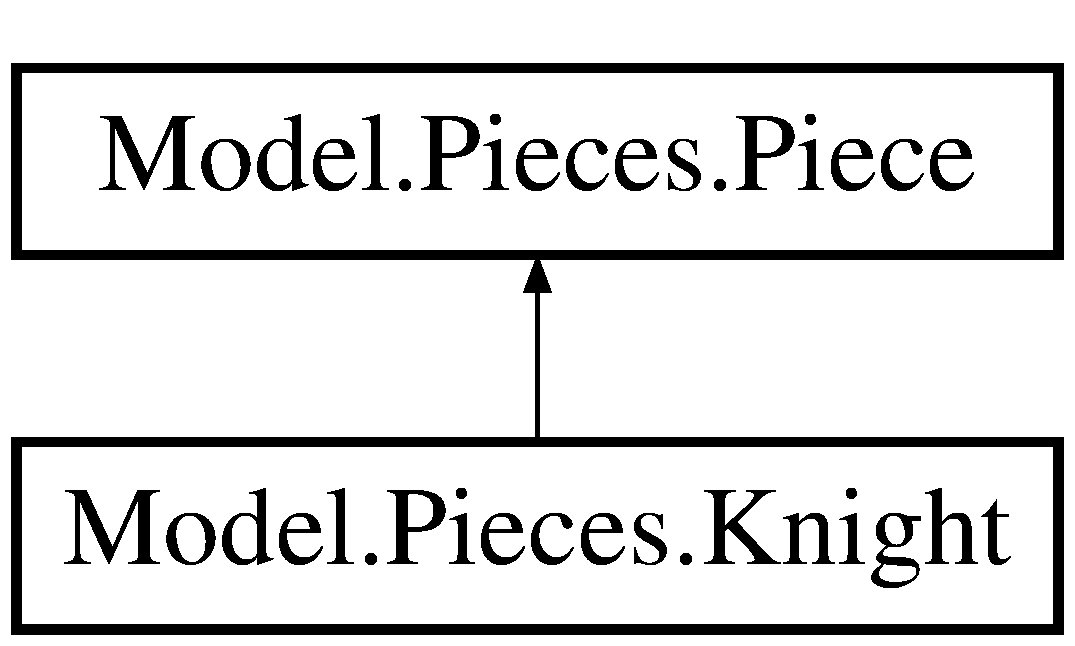
\includegraphics[height=2.000000cm]{class_model_1_1_pieces_1_1_knight}
\end{center}
\end{figure}
\subsection*{Public Member Functions}
\begin{DoxyCompactItemize}
\item 
\hyperlink{class_model_1_1_pieces_1_1_knight_a8e99ebaed34bfc3465a5d577fb0692a9}{Knight} (\hyperlink{class_model_1_1_team}{Team} team, int x\+Value, int y\+Value)
\item 
boolean \hyperlink{class_model_1_1_pieces_1_1_knight_a205e4f1df4e275380734cca239495979}{is\+Valid\+Move} (\hyperlink{class_model_1_1_move}{Move} move, \hyperlink{class_model_1_1_board}{Board} board)
\item 
boolean \hyperlink{class_model_1_1_pieces_1_1_knight_ae8502fc00e75878195898f12e8ada235}{has\+No\+Piece\+In\+Movement\+Route} (\hyperlink{class_model_1_1_move}{Move} move, \hyperlink{class_model_1_1_board}{Board} board)
\item 
List$<$ \hyperlink{class_model_1_1_move}{Move} $>$ \hyperlink{class_model_1_1_pieces_1_1_knight_ab020b621de20f10e1e9c753d9cd71342}{find\+All\+Moves} (\hyperlink{class_model_1_1_board}{Board} board)
\end{DoxyCompactItemize}


\subsection{Detailed Description}
\hyperlink{class_model_1_1_pieces_1_1_knight}{Knight} class to describe \hyperlink{class_model_1_1_pieces_1_1_knight}{Knight}\textquotesingle{}s possible moves. \begin{DoxyAuthor}{Author}
arnavmishra 
\end{DoxyAuthor}


\subsection{Constructor \& Destructor Documentation}
\hypertarget{class_model_1_1_pieces_1_1_knight_a8e99ebaed34bfc3465a5d577fb0692a9}{}\label{class_model_1_1_pieces_1_1_knight_a8e99ebaed34bfc3465a5d577fb0692a9} 
\index{Model\+::\+Pieces\+::\+Knight@{Model\+::\+Pieces\+::\+Knight}!Knight@{Knight}}
\index{Knight@{Knight}!Model\+::\+Pieces\+::\+Knight@{Model\+::\+Pieces\+::\+Knight}}
\subsubsection{\texorpdfstring{Knight()}{Knight()}}
{\footnotesize\ttfamily Model.\+Pieces.\+Knight.\+Knight (\begin{DoxyParamCaption}\item[{\hyperlink{class_model_1_1_team}{Team}}]{team,  }\item[{int}]{x\+Value,  }\item[{int}]{y\+Value }\end{DoxyParamCaption})}

Constructor to initialize \hyperlink{class_model_1_1_pieces_1_1_knight}{Knight} on a team and coordinate. 
\begin{DoxyParams}{Parameters}
{\em team} & \\
\hline
\end{DoxyParams}


\subsection{Member Function Documentation}
\hypertarget{class_model_1_1_pieces_1_1_knight_ab020b621de20f10e1e9c753d9cd71342}{}\label{class_model_1_1_pieces_1_1_knight_ab020b621de20f10e1e9c753d9cd71342} 
\index{Model\+::\+Pieces\+::\+Knight@{Model\+::\+Pieces\+::\+Knight}!find\+All\+Moves@{find\+All\+Moves}}
\index{find\+All\+Moves@{find\+All\+Moves}!Model\+::\+Pieces\+::\+Knight@{Model\+::\+Pieces\+::\+Knight}}
\subsubsection{\texorpdfstring{find\+All\+Moves()}{findAllMoves()}}
{\footnotesize\ttfamily List$<$\hyperlink{class_model_1_1_move}{Move}$>$ Model.\+Pieces.\+Knight.\+find\+All\+Moves (\begin{DoxyParamCaption}\item[{\hyperlink{class_model_1_1_board}{Board}}]{board }\end{DoxyParamCaption})}

Function to get all valid possible moves for the \hyperlink{class_model_1_1_pieces_1_1_knight}{Knight} in any direction. 
\begin{DoxyParams}{Parameters}
{\em board} & \\
\hline
\end{DoxyParams}
\begin{DoxyReturn}{Returns}
all possible valid moves. 
\end{DoxyReturn}
\hypertarget{class_model_1_1_pieces_1_1_knight_ae8502fc00e75878195898f12e8ada235}{}\label{class_model_1_1_pieces_1_1_knight_ae8502fc00e75878195898f12e8ada235} 
\index{Model\+::\+Pieces\+::\+Knight@{Model\+::\+Pieces\+::\+Knight}!has\+No\+Piece\+In\+Movement\+Route@{has\+No\+Piece\+In\+Movement\+Route}}
\index{has\+No\+Piece\+In\+Movement\+Route@{has\+No\+Piece\+In\+Movement\+Route}!Model\+::\+Pieces\+::\+Knight@{Model\+::\+Pieces\+::\+Knight}}
\subsubsection{\texorpdfstring{has\+No\+Piece\+In\+Movement\+Route()}{hasNoPieceInMovementRoute()}}
{\footnotesize\ttfamily boolean Model.\+Pieces.\+Knight.\+has\+No\+Piece\+In\+Movement\+Route (\begin{DoxyParamCaption}\item[{\hyperlink{class_model_1_1_move}{Move}}]{move,  }\item[{\hyperlink{class_model_1_1_board}{Board}}]{board }\end{DoxyParamCaption})}

The knight is allowed to jump over pieces. 
\begin{DoxyParams}{Parameters}
{\em move} & \\
\hline
{\em board} & \\
\hline
\end{DoxyParams}
\begin{DoxyReturn}{Returns}
whether the knight leaps over pieces. 
\end{DoxyReturn}
\hypertarget{class_model_1_1_pieces_1_1_knight_a205e4f1df4e275380734cca239495979}{}\label{class_model_1_1_pieces_1_1_knight_a205e4f1df4e275380734cca239495979} 
\index{Model\+::\+Pieces\+::\+Knight@{Model\+::\+Pieces\+::\+Knight}!is\+Valid\+Move@{is\+Valid\+Move}}
\index{is\+Valid\+Move@{is\+Valid\+Move}!Model\+::\+Pieces\+::\+Knight@{Model\+::\+Pieces\+::\+Knight}}
\subsubsection{\texorpdfstring{is\+Valid\+Move()}{isValidMove()}}
{\footnotesize\ttfamily boolean Model.\+Pieces.\+Knight.\+is\+Valid\+Move (\begin{DoxyParamCaption}\item[{\hyperlink{class_model_1_1_move}{Move}}]{move,  }\item[{\hyperlink{class_model_1_1_board}{Board}}]{board }\end{DoxyParamCaption})}

Function to check whether a knight\textquotesingle{}s move is valid. 
\begin{DoxyParams}{Parameters}
{\em move} & \\
\hline
{\em board} & \\
\hline
\end{DoxyParams}
\begin{DoxyReturn}{Returns}
Whether the move is valid. 
\end{DoxyReturn}


The documentation for this class was generated from the following file\+:\begin{DoxyCompactItemize}
\item 
src/\+Model/\+Pieces/Knight.\+java\end{DoxyCompactItemize}

\hypertarget{class_tests_1_1_knight_test}{}\section{Tests.\+Knight\+Test Class Reference}
\label{class_tests_1_1_knight_test}\index{Tests.\+Knight\+Test@{Tests.\+Knight\+Test}}
\subsection*{Public Member Functions}
\begin{DoxyCompactItemize}
\item 
void \hyperlink{class_tests_1_1_knight_test_aeef4aecba7d22407c8945dabf02ae3fa}{valid\+Knight\+Movement} ()  throws Exception 
\item 
void \hyperlink{class_tests_1_1_knight_test_a2055e2c815f2c80d89a9f9519702b712}{invalid\+Knight\+Movement} ()  throws Exception 
\item 
void \hyperlink{class_tests_1_1_knight_test_a1f2b34d555e7c732d14245368341ee02}{correct\+All\+Starting\+Knight\+Moves} ()  throws Exception 
\end{DoxyCompactItemize}


\subsection{Detailed Description}
Tests for the Knight class. \begin{DoxyAuthor}{Author}
arnavmishra 
\end{DoxyAuthor}


\subsection{Member Function Documentation}
\hypertarget{class_tests_1_1_knight_test_a1f2b34d555e7c732d14245368341ee02}{}\label{class_tests_1_1_knight_test_a1f2b34d555e7c732d14245368341ee02} 
\index{Tests\+::\+Knight\+Test@{Tests\+::\+Knight\+Test}!correct\+All\+Starting\+Knight\+Moves@{correct\+All\+Starting\+Knight\+Moves}}
\index{correct\+All\+Starting\+Knight\+Moves@{correct\+All\+Starting\+Knight\+Moves}!Tests\+::\+Knight\+Test@{Tests\+::\+Knight\+Test}}
\subsubsection{\texorpdfstring{correct\+All\+Starting\+Knight\+Moves()}{correctAllStartingKnightMoves()}}
{\footnotesize\ttfamily void Tests.\+Knight\+Test.\+correct\+All\+Starting\+Knight\+Moves (\begin{DoxyParamCaption}{ }\end{DoxyParamCaption}) throws Exception}

Test to confirm that all possible knight moves are available by checking that the knight has all starting moves listed. 
\begin{DoxyExceptions}{Exceptions}
{\em Exception} & \\
\hline
\end{DoxyExceptions}
\hypertarget{class_tests_1_1_knight_test_a2055e2c815f2c80d89a9f9519702b712}{}\label{class_tests_1_1_knight_test_a2055e2c815f2c80d89a9f9519702b712} 
\index{Tests\+::\+Knight\+Test@{Tests\+::\+Knight\+Test}!invalid\+Knight\+Movement@{invalid\+Knight\+Movement}}
\index{invalid\+Knight\+Movement@{invalid\+Knight\+Movement}!Tests\+::\+Knight\+Test@{Tests\+::\+Knight\+Test}}
\subsubsection{\texorpdfstring{invalid\+Knight\+Movement()}{invalidKnightMovement()}}
{\footnotesize\ttfamily void Tests.\+Knight\+Test.\+invalid\+Knight\+Movement (\begin{DoxyParamCaption}{ }\end{DoxyParamCaption}) throws Exception}

Test to check invalid knight movement by moving a knight diagonally. 
\begin{DoxyExceptions}{Exceptions}
{\em Exception} & \\
\hline
\end{DoxyExceptions}
\hypertarget{class_tests_1_1_knight_test_aeef4aecba7d22407c8945dabf02ae3fa}{}\label{class_tests_1_1_knight_test_aeef4aecba7d22407c8945dabf02ae3fa} 
\index{Tests\+::\+Knight\+Test@{Tests\+::\+Knight\+Test}!valid\+Knight\+Movement@{valid\+Knight\+Movement}}
\index{valid\+Knight\+Movement@{valid\+Knight\+Movement}!Tests\+::\+Knight\+Test@{Tests\+::\+Knight\+Test}}
\subsubsection{\texorpdfstring{valid\+Knight\+Movement()}{validKnightMovement()}}
{\footnotesize\ttfamily void Tests.\+Knight\+Test.\+valid\+Knight\+Movement (\begin{DoxyParamCaption}{ }\end{DoxyParamCaption}) throws Exception}

Test to confirm valid knight movement by moving a knight up two, left one. 
\begin{DoxyExceptions}{Exceptions}
{\em Exception} & \\
\hline
\end{DoxyExceptions}


The documentation for this class was generated from the following file\+:\begin{DoxyCompactItemize}
\item 
src/\+Tests/Knight\+Test.\+java\end{DoxyCompactItemize}

\hypertarget{class_model_1_1_move}{}\section{Model.\+Move Class Reference}
\label{class_model_1_1_move}\index{Model.\+Move@{Model.\+Move}}
\subsection*{Public Member Functions}
\begin{DoxyCompactItemize}
\item 
\hyperlink{class_model_1_1_move_aab0a02c388b5980cee0e9a2a527504a5}{Move} (int startX, int startY, int endX, int endY, int team)
\item 
int \hyperlink{class_model_1_1_move_ad7b5aacb5a63ce66b88462cb14226511}{get\+StartX} ()
\item 
int \hyperlink{class_model_1_1_move_a28f467365161a5946531359210c8819c}{get\+EndX} ()
\item 
int \hyperlink{class_model_1_1_move_a4bbb121acdea24249ee7ea4466fd8e7a}{get\+StartY} ()
\item 
int \hyperlink{class_model_1_1_move_a35fb048c2ba8223df87a13994d7f37a3}{get\+EndY} ()
\item 
int \hyperlink{class_model_1_1_move_adca5d2e7181293d311eca9062b4f9d1e}{get\+Team\+Number} ()
\end{DoxyCompactItemize}


\subsection{Constructor \& Destructor Documentation}
\hypertarget{class_model_1_1_move_aab0a02c388b5980cee0e9a2a527504a5}{}\label{class_model_1_1_move_aab0a02c388b5980cee0e9a2a527504a5} 
\index{Model\+::\+Move@{Model\+::\+Move}!Move@{Move}}
\index{Move@{Move}!Model\+::\+Move@{Model\+::\+Move}}
\subsubsection{\texorpdfstring{Move()}{Move()}}
{\footnotesize\ttfamily Model.\+Move.\+Move (\begin{DoxyParamCaption}\item[{int}]{startX,  }\item[{int}]{startY,  }\item[{int}]{endX,  }\item[{int}]{endY,  }\item[{int}]{team }\end{DoxyParamCaption})}

Constructor to initialize move object. 
\begin{DoxyParams}{Parameters}
{\em startX} & \\
\hline
{\em startY} & \\
\hline
{\em endX} & \\
\hline
{\em endY} & \\
\hline
{\em team} & \\
\hline
\end{DoxyParams}


\subsection{Member Function Documentation}
\hypertarget{class_model_1_1_move_a28f467365161a5946531359210c8819c}{}\label{class_model_1_1_move_a28f467365161a5946531359210c8819c} 
\index{Model\+::\+Move@{Model\+::\+Move}!get\+EndX@{get\+EndX}}
\index{get\+EndX@{get\+EndX}!Model\+::\+Move@{Model\+::\+Move}}
\subsubsection{\texorpdfstring{get\+End\+X()}{getEndX()}}
{\footnotesize\ttfamily int Model.\+Move.\+get\+EndX (\begin{DoxyParamCaption}{ }\end{DoxyParamCaption})}

Getter for end X coordinate. \begin{DoxyReturn}{Returns}
end X coordinate. 
\end{DoxyReturn}
\hypertarget{class_model_1_1_move_a35fb048c2ba8223df87a13994d7f37a3}{}\label{class_model_1_1_move_a35fb048c2ba8223df87a13994d7f37a3} 
\index{Model\+::\+Move@{Model\+::\+Move}!get\+EndY@{get\+EndY}}
\index{get\+EndY@{get\+EndY}!Model\+::\+Move@{Model\+::\+Move}}
\subsubsection{\texorpdfstring{get\+End\+Y()}{getEndY()}}
{\footnotesize\ttfamily int Model.\+Move.\+get\+EndY (\begin{DoxyParamCaption}{ }\end{DoxyParamCaption})}

Getter for end Y coordinate. \begin{DoxyReturn}{Returns}
end Y coordinate. 
\end{DoxyReturn}
\hypertarget{class_model_1_1_move_ad7b5aacb5a63ce66b88462cb14226511}{}\label{class_model_1_1_move_ad7b5aacb5a63ce66b88462cb14226511} 
\index{Model\+::\+Move@{Model\+::\+Move}!get\+StartX@{get\+StartX}}
\index{get\+StartX@{get\+StartX}!Model\+::\+Move@{Model\+::\+Move}}
\subsubsection{\texorpdfstring{get\+Start\+X()}{getStartX()}}
{\footnotesize\ttfamily int Model.\+Move.\+get\+StartX (\begin{DoxyParamCaption}{ }\end{DoxyParamCaption})}

Getter for starting X coordinate. \begin{DoxyReturn}{Returns}
starting X coordinate. 
\end{DoxyReturn}
\hypertarget{class_model_1_1_move_a4bbb121acdea24249ee7ea4466fd8e7a}{}\label{class_model_1_1_move_a4bbb121acdea24249ee7ea4466fd8e7a} 
\index{Model\+::\+Move@{Model\+::\+Move}!get\+StartY@{get\+StartY}}
\index{get\+StartY@{get\+StartY}!Model\+::\+Move@{Model\+::\+Move}}
\subsubsection{\texorpdfstring{get\+Start\+Y()}{getStartY()}}
{\footnotesize\ttfamily int Model.\+Move.\+get\+StartY (\begin{DoxyParamCaption}{ }\end{DoxyParamCaption})}

Getter for starting Y coordinate. \begin{DoxyReturn}{Returns}
starting Y coordinate. 
\end{DoxyReturn}
\hypertarget{class_model_1_1_move_adca5d2e7181293d311eca9062b4f9d1e}{}\label{class_model_1_1_move_adca5d2e7181293d311eca9062b4f9d1e} 
\index{Model\+::\+Move@{Model\+::\+Move}!get\+Team\+Number@{get\+Team\+Number}}
\index{get\+Team\+Number@{get\+Team\+Number}!Model\+::\+Move@{Model\+::\+Move}}
\subsubsection{\texorpdfstring{get\+Team\+Number()}{getTeamNumber()}}
{\footnotesize\ttfamily int Model.\+Move.\+get\+Team\+Number (\begin{DoxyParamCaption}{ }\end{DoxyParamCaption})}

Getter for move\textquotesingle{}s team number. \begin{DoxyReturn}{Returns}
move\textquotesingle{}s team number. 
\end{DoxyReturn}


The documentation for this class was generated from the following file\+:\begin{DoxyCompactItemize}
\item 
src/\+Model/Move.\+java\end{DoxyCompactItemize}

\hypertarget{class_model_1_1_pieces_1_1_pawn}{}\section{Model.\+Pieces.\+Pawn Class Reference}
\label{class_model_1_1_pieces_1_1_pawn}\index{Model.\+Pieces.\+Pawn@{Model.\+Pieces.\+Pawn}}
Inheritance diagram for Model.\+Pieces.\+Pawn\+:\begin{figure}[H]
\begin{center}
\leavevmode
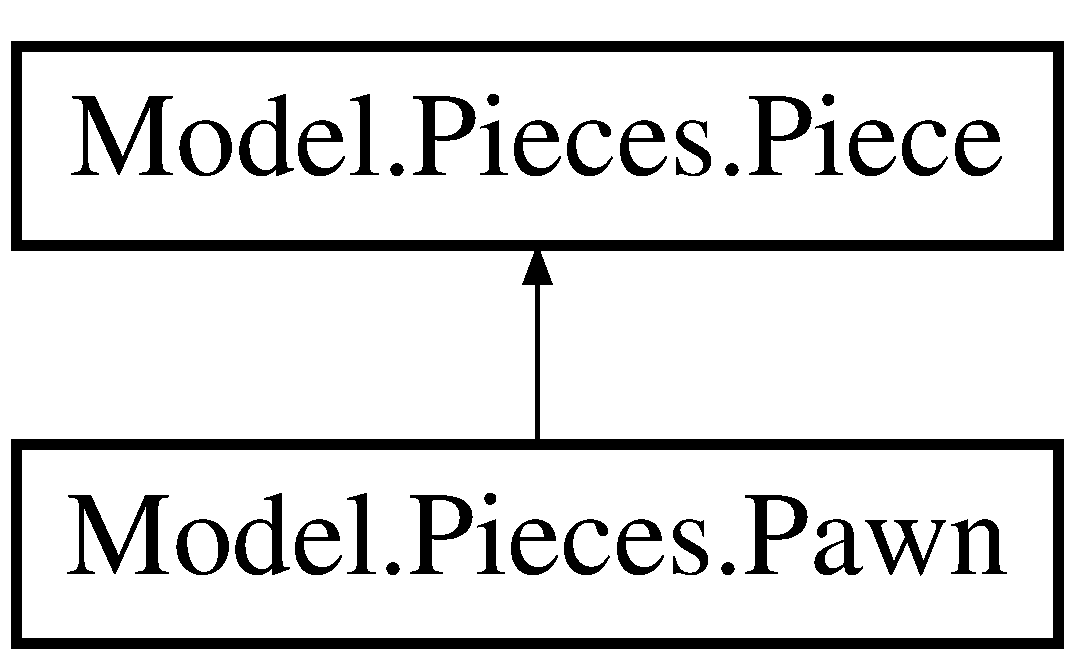
\includegraphics[height=2.000000cm]{class_model_1_1_pieces_1_1_pawn}
\end{center}
\end{figure}
\subsection*{Public Member Functions}
\begin{DoxyCompactItemize}
\item 
\hyperlink{class_model_1_1_pieces_1_1_pawn_ad3d3d740e79b02e16c5cc4b2da2f25bf}{Pawn} (\hyperlink{class_model_1_1_team}{Team} team, int x\+Value, int y\+Value)
\item 
boolean \hyperlink{class_model_1_1_pieces_1_1_pawn_a8bb2d90244e6992f8c24108d2a8c13e7}{is\+Valid\+Move} (\hyperlink{class_model_1_1_move}{Move} move, \hyperlink{class_model_1_1_board}{Board} board)
\item 
boolean \hyperlink{class_model_1_1_pieces_1_1_pawn_a92db7183e3d916aa6aed7c9a7cf89ba3}{check\+No\+Piece} (\hyperlink{class_model_1_1_move}{Move} move, \hyperlink{class_model_1_1_board}{Board} board)
\item 
boolean \hyperlink{class_model_1_1_pieces_1_1_pawn_a1088583c9809266ccefc49ce8d272d24}{check\+Forward} (\hyperlink{class_model_1_1_move}{Move} move, int y\+Delta)
\item 
boolean \hyperlink{class_model_1_1_pieces_1_1_pawn_a130ca7b5f609a5caf2e76e782efc30c4}{opponent\+Piece} (\hyperlink{class_model_1_1_move}{Move} move, \hyperlink{class_model_1_1_board}{Board} board)
\item 
boolean \hyperlink{class_model_1_1_pieces_1_1_pawn_a051caa0213913b8c3748f47a5bdfcab6}{has\+No\+Piece\+In\+Movement\+Route} (\hyperlink{class_model_1_1_move}{Move} move, \hyperlink{class_model_1_1_board}{Board} board)
\item 
List$<$ \hyperlink{class_model_1_1_move}{Move} $>$ \hyperlink{class_model_1_1_pieces_1_1_pawn_a95dcb404b5207a813149c152d3a48a50}{find\+All\+Moves} (\hyperlink{class_model_1_1_board}{Board} board)
\end{DoxyCompactItemize}


\subsection{Detailed Description}
\hyperlink{class_model_1_1_pieces_1_1_pawn}{Pawn} class to describe \hyperlink{class_model_1_1_pieces_1_1_pawn}{Pawn}\textquotesingle{}s possible moves. \begin{DoxyAuthor}{Author}
arnavmishra 
\end{DoxyAuthor}


\subsection{Constructor \& Destructor Documentation}
\hypertarget{class_model_1_1_pieces_1_1_pawn_ad3d3d740e79b02e16c5cc4b2da2f25bf}{}\label{class_model_1_1_pieces_1_1_pawn_ad3d3d740e79b02e16c5cc4b2da2f25bf} 
\index{Model\+::\+Pieces\+::\+Pawn@{Model\+::\+Pieces\+::\+Pawn}!Pawn@{Pawn}}
\index{Pawn@{Pawn}!Model\+::\+Pieces\+::\+Pawn@{Model\+::\+Pieces\+::\+Pawn}}
\subsubsection{\texorpdfstring{Pawn()}{Pawn()}}
{\footnotesize\ttfamily Model.\+Pieces.\+Pawn.\+Pawn (\begin{DoxyParamCaption}\item[{\hyperlink{class_model_1_1_team}{Team}}]{team,  }\item[{int}]{x\+Value,  }\item[{int}]{y\+Value }\end{DoxyParamCaption})}

Constructor to initialize \hyperlink{class_model_1_1_pieces_1_1_pawn}{Pawn} on a team and coordinate. 
\begin{DoxyParams}{Parameters}
{\em team} & \\
\hline
\end{DoxyParams}


\subsection{Member Function Documentation}
\hypertarget{class_model_1_1_pieces_1_1_pawn_a1088583c9809266ccefc49ce8d272d24}{}\label{class_model_1_1_pieces_1_1_pawn_a1088583c9809266ccefc49ce8d272d24} 
\index{Model\+::\+Pieces\+::\+Pawn@{Model\+::\+Pieces\+::\+Pawn}!check\+Forward@{check\+Forward}}
\index{check\+Forward@{check\+Forward}!Model\+::\+Pieces\+::\+Pawn@{Model\+::\+Pieces\+::\+Pawn}}
\subsubsection{\texorpdfstring{check\+Forward()}{checkForward()}}
{\footnotesize\ttfamily boolean Model.\+Pieces.\+Pawn.\+check\+Forward (\begin{DoxyParamCaption}\item[{\hyperlink{class_model_1_1_move}{Move}}]{move,  }\item[{int}]{y\+Delta }\end{DoxyParamCaption})}

Check that the pawn is moving forward depending on which team it is on. 
\begin{DoxyParams}{Parameters}
{\em move} & \\
\hline
{\em y\+Delta} & \\
\hline
\end{DoxyParams}
\begin{DoxyReturn}{Returns}
whether the pawn is moving forward 
\end{DoxyReturn}
\hypertarget{class_model_1_1_pieces_1_1_pawn_a92db7183e3d916aa6aed7c9a7cf89ba3}{}\label{class_model_1_1_pieces_1_1_pawn_a92db7183e3d916aa6aed7c9a7cf89ba3} 
\index{Model\+::\+Pieces\+::\+Pawn@{Model\+::\+Pieces\+::\+Pawn}!check\+No\+Piece@{check\+No\+Piece}}
\index{check\+No\+Piece@{check\+No\+Piece}!Model\+::\+Pieces\+::\+Pawn@{Model\+::\+Pieces\+::\+Pawn}}
\subsubsection{\texorpdfstring{check\+No\+Piece()}{checkNoPiece()}}
{\footnotesize\ttfamily boolean Model.\+Pieces.\+Pawn.\+check\+No\+Piece (\begin{DoxyParamCaption}\item[{\hyperlink{class_model_1_1_move}{Move}}]{move,  }\item[{\hyperlink{class_model_1_1_board}{Board}}]{board }\end{DoxyParamCaption})}

Helper function to confirm that there is no piece where the pawn is moving for forward movement. 
\begin{DoxyParams}{Parameters}
{\em move} & \\
\hline
{\em board} & \\
\hline
\end{DoxyParams}
\begin{DoxyReturn}{Returns}
whether there is already a piece at the destination 
\end{DoxyReturn}
\hypertarget{class_model_1_1_pieces_1_1_pawn_a95dcb404b5207a813149c152d3a48a50}{}\label{class_model_1_1_pieces_1_1_pawn_a95dcb404b5207a813149c152d3a48a50} 
\index{Model\+::\+Pieces\+::\+Pawn@{Model\+::\+Pieces\+::\+Pawn}!find\+All\+Moves@{find\+All\+Moves}}
\index{find\+All\+Moves@{find\+All\+Moves}!Model\+::\+Pieces\+::\+Pawn@{Model\+::\+Pieces\+::\+Pawn}}
\subsubsection{\texorpdfstring{find\+All\+Moves()}{findAllMoves()}}
{\footnotesize\ttfamily List$<$\hyperlink{class_model_1_1_move}{Move}$>$ Model.\+Pieces.\+Pawn.\+find\+All\+Moves (\begin{DoxyParamCaption}\item[{\hyperlink{class_model_1_1_board}{Board}}]{board }\end{DoxyParamCaption})}

Function to get all valid possible moves for the \hyperlink{class_model_1_1_pieces_1_1_pawn}{Pawn} in any direction. 
\begin{DoxyParams}{Parameters}
{\em board} & \\
\hline
\end{DoxyParams}
\begin{DoxyReturn}{Returns}
all possible valid moves. 
\end{DoxyReturn}
\hypertarget{class_model_1_1_pieces_1_1_pawn_a051caa0213913b8c3748f47a5bdfcab6}{}\label{class_model_1_1_pieces_1_1_pawn_a051caa0213913b8c3748f47a5bdfcab6} 
\index{Model\+::\+Pieces\+::\+Pawn@{Model\+::\+Pieces\+::\+Pawn}!has\+No\+Piece\+In\+Movement\+Route@{has\+No\+Piece\+In\+Movement\+Route}}
\index{has\+No\+Piece\+In\+Movement\+Route@{has\+No\+Piece\+In\+Movement\+Route}!Model\+::\+Pieces\+::\+Pawn@{Model\+::\+Pieces\+::\+Pawn}}
\subsubsection{\texorpdfstring{has\+No\+Piece\+In\+Movement\+Route()}{hasNoPieceInMovementRoute()}}
{\footnotesize\ttfamily boolean Model.\+Pieces.\+Pawn.\+has\+No\+Piece\+In\+Movement\+Route (\begin{DoxyParamCaption}\item[{\hyperlink{class_model_1_1_move}{Move}}]{move,  }\item[{\hyperlink{class_model_1_1_board}{Board}}]{board }\end{DoxyParamCaption})}

Check that the pawn doesn\textquotesingle{}t jump over any piece. 
\begin{DoxyParams}{Parameters}
{\em move} & \\
\hline
{\em board} & \\
\hline
\end{DoxyParams}
\begin{DoxyReturn}{Returns}
whether the pawn leaps over pieces. 
\end{DoxyReturn}
\hypertarget{class_model_1_1_pieces_1_1_pawn_a8bb2d90244e6992f8c24108d2a8c13e7}{}\label{class_model_1_1_pieces_1_1_pawn_a8bb2d90244e6992f8c24108d2a8c13e7} 
\index{Model\+::\+Pieces\+::\+Pawn@{Model\+::\+Pieces\+::\+Pawn}!is\+Valid\+Move@{is\+Valid\+Move}}
\index{is\+Valid\+Move@{is\+Valid\+Move}!Model\+::\+Pieces\+::\+Pawn@{Model\+::\+Pieces\+::\+Pawn}}
\subsubsection{\texorpdfstring{is\+Valid\+Move()}{isValidMove()}}
{\footnotesize\ttfamily boolean Model.\+Pieces.\+Pawn.\+is\+Valid\+Move (\begin{DoxyParamCaption}\item[{\hyperlink{class_model_1_1_move}{Move}}]{move,  }\item[{\hyperlink{class_model_1_1_board}{Board}}]{board }\end{DoxyParamCaption})}

Function to check whether a pawn\textquotesingle{}s move is valid. 
\begin{DoxyParams}{Parameters}
{\em move} & \\
\hline
{\em board} & \\
\hline
\end{DoxyParams}
\begin{DoxyReturn}{Returns}
Whether the move is valid. 
\end{DoxyReturn}
\hypertarget{class_model_1_1_pieces_1_1_pawn_a130ca7b5f609a5caf2e76e782efc30c4}{}\label{class_model_1_1_pieces_1_1_pawn_a130ca7b5f609a5caf2e76e782efc30c4} 
\index{Model\+::\+Pieces\+::\+Pawn@{Model\+::\+Pieces\+::\+Pawn}!opponent\+Piece@{opponent\+Piece}}
\index{opponent\+Piece@{opponent\+Piece}!Model\+::\+Pieces\+::\+Pawn@{Model\+::\+Pieces\+::\+Pawn}}
\subsubsection{\texorpdfstring{opponent\+Piece()}{opponentPiece()}}
{\footnotesize\ttfamily boolean Model.\+Pieces.\+Pawn.\+opponent\+Piece (\begin{DoxyParamCaption}\item[{\hyperlink{class_model_1_1_move}{Move}}]{move,  }\item[{\hyperlink{class_model_1_1_board}{Board}}]{board }\end{DoxyParamCaption})}

Check that the pawn is taking an opponent piece if it is moving diagonally. 
\begin{DoxyParams}{Parameters}
{\em move} & \\
\hline
{\em board} & \\
\hline
\end{DoxyParams}
\begin{DoxyReturn}{Returns}
whether there is an opponent piece diagonally 
\end{DoxyReturn}


The documentation for this class was generated from the following file\+:\begin{DoxyCompactItemize}
\item 
src/\+Model/\+Pieces/Pawn.\+java\end{DoxyCompactItemize}

\hypertarget{class_tests_1_1_pawn_test}{}\section{Tests.\+Pawn\+Test Class Reference}
\label{class_tests_1_1_pawn_test}\index{Tests.\+Pawn\+Test@{Tests.\+Pawn\+Test}}
\subsection*{Public Member Functions}
\begin{DoxyCompactItemize}
\item 
void \hyperlink{class_tests_1_1_pawn_test_afc62c7df60ea48714139aa3b1fdec002}{valid\+Pawn\+Single\+Space\+Movement} ()  throws Exception 
\item 
void \hyperlink{class_tests_1_1_pawn_test_a609983048db9ea8be85c1a0eca1a4c64}{valid\+Pawn\+Double\+Space\+Movement\+From\+Start} ()  throws Exception 
\item 
void \hyperlink{class_tests_1_1_pawn_test_a62b592bc182e06d091c635fd46cf835b}{invalid\+Pawn\+Double\+Space\+Movement\+From\+Other\+Position} ()  throws Exception 
\item 
void \hyperlink{class_tests_1_1_pawn_test_aee76762875ad44ca3a078618467f4e87}{valid\+Pawn\+Diagonal\+Movement} ()  throws Exception 
\item 
void \hyperlink{class_tests_1_1_pawn_test_a5de98c4a33ad5690dda92cebdf5612a4}{invalid\+Pawn\+Diagonal\+Movement} ()  throws Exception 
\item 
void \hyperlink{class_tests_1_1_pawn_test_abddfebe793102a67725109bbe1a3ca31}{correct\+All\+Starting\+Pawn\+Moves} ()  throws Exception 
\end{DoxyCompactItemize}


\subsection{Detailed Description}
Tests for the Pawn class. \begin{DoxyAuthor}{Author}
arnavmishra 
\end{DoxyAuthor}


\subsection{Member Function Documentation}
\hypertarget{class_tests_1_1_pawn_test_abddfebe793102a67725109bbe1a3ca31}{}\label{class_tests_1_1_pawn_test_abddfebe793102a67725109bbe1a3ca31} 
\index{Tests\+::\+Pawn\+Test@{Tests\+::\+Pawn\+Test}!correct\+All\+Starting\+Pawn\+Moves@{correct\+All\+Starting\+Pawn\+Moves}}
\index{correct\+All\+Starting\+Pawn\+Moves@{correct\+All\+Starting\+Pawn\+Moves}!Tests\+::\+Pawn\+Test@{Tests\+::\+Pawn\+Test}}
\subsubsection{\texorpdfstring{correct\+All\+Starting\+Pawn\+Moves()}{correctAllStartingPawnMoves()}}
{\footnotesize\ttfamily void Tests.\+Pawn\+Test.\+correct\+All\+Starting\+Pawn\+Moves (\begin{DoxyParamCaption}{ }\end{DoxyParamCaption}) throws Exception}

Test to confirm that all possible movements for a pawn are found from starting position. 
\begin{DoxyExceptions}{Exceptions}
{\em Exception} & \\
\hline
\end{DoxyExceptions}
\hypertarget{class_tests_1_1_pawn_test_a5de98c4a33ad5690dda92cebdf5612a4}{}\label{class_tests_1_1_pawn_test_a5de98c4a33ad5690dda92cebdf5612a4} 
\index{Tests\+::\+Pawn\+Test@{Tests\+::\+Pawn\+Test}!invalid\+Pawn\+Diagonal\+Movement@{invalid\+Pawn\+Diagonal\+Movement}}
\index{invalid\+Pawn\+Diagonal\+Movement@{invalid\+Pawn\+Diagonal\+Movement}!Tests\+::\+Pawn\+Test@{Tests\+::\+Pawn\+Test}}
\subsubsection{\texorpdfstring{invalid\+Pawn\+Diagonal\+Movement()}{invalidPawnDiagonalMovement()}}
{\footnotesize\ttfamily void Tests.\+Pawn\+Test.\+invalid\+Pawn\+Diagonal\+Movement (\begin{DoxyParamCaption}{ }\end{DoxyParamCaption}) throws Exception}

Test to ensure a pawn cannot move diagonally if the diagonal position doesn\textquotesingle{}t have an opposing team. 
\begin{DoxyExceptions}{Exceptions}
{\em Exception} & \\
\hline
\end{DoxyExceptions}
\hypertarget{class_tests_1_1_pawn_test_a62b592bc182e06d091c635fd46cf835b}{}\label{class_tests_1_1_pawn_test_a62b592bc182e06d091c635fd46cf835b} 
\index{Tests\+::\+Pawn\+Test@{Tests\+::\+Pawn\+Test}!invalid\+Pawn\+Double\+Space\+Movement\+From\+Other\+Position@{invalid\+Pawn\+Double\+Space\+Movement\+From\+Other\+Position}}
\index{invalid\+Pawn\+Double\+Space\+Movement\+From\+Other\+Position@{invalid\+Pawn\+Double\+Space\+Movement\+From\+Other\+Position}!Tests\+::\+Pawn\+Test@{Tests\+::\+Pawn\+Test}}
\subsubsection{\texorpdfstring{invalid\+Pawn\+Double\+Space\+Movement\+From\+Other\+Position()}{invalidPawnDoubleSpaceMovementFromOtherPosition()}}
{\footnotesize\ttfamily void Tests.\+Pawn\+Test.\+invalid\+Pawn\+Double\+Space\+Movement\+From\+Other\+Position (\begin{DoxyParamCaption}{ }\end{DoxyParamCaption}) throws Exception}

Test to check a Pawn cannot move forward two spaces from a non-\/starting space by moving a Pawn up one space and then trying to move it up two spaces. 
\begin{DoxyExceptions}{Exceptions}
{\em Exception} & \\
\hline
\end{DoxyExceptions}
\hypertarget{class_tests_1_1_pawn_test_aee76762875ad44ca3a078618467f4e87}{}\label{class_tests_1_1_pawn_test_aee76762875ad44ca3a078618467f4e87} 
\index{Tests\+::\+Pawn\+Test@{Tests\+::\+Pawn\+Test}!valid\+Pawn\+Diagonal\+Movement@{valid\+Pawn\+Diagonal\+Movement}}
\index{valid\+Pawn\+Diagonal\+Movement@{valid\+Pawn\+Diagonal\+Movement}!Tests\+::\+Pawn\+Test@{Tests\+::\+Pawn\+Test}}
\subsubsection{\texorpdfstring{valid\+Pawn\+Diagonal\+Movement()}{validPawnDiagonalMovement()}}
{\footnotesize\ttfamily void Tests.\+Pawn\+Test.\+valid\+Pawn\+Diagonal\+Movement (\begin{DoxyParamCaption}{ }\end{DoxyParamCaption}) throws Exception}

Test to check a pawn\textquotesingle{}s diagonal movement by setting up the board with two opposing pawns diagonal from each other and ensuring the movement is allowed. 
\begin{DoxyExceptions}{Exceptions}
{\em Exception} & \\
\hline
\end{DoxyExceptions}
\hypertarget{class_tests_1_1_pawn_test_a609983048db9ea8be85c1a0eca1a4c64}{}\label{class_tests_1_1_pawn_test_a609983048db9ea8be85c1a0eca1a4c64} 
\index{Tests\+::\+Pawn\+Test@{Tests\+::\+Pawn\+Test}!valid\+Pawn\+Double\+Space\+Movement\+From\+Start@{valid\+Pawn\+Double\+Space\+Movement\+From\+Start}}
\index{valid\+Pawn\+Double\+Space\+Movement\+From\+Start@{valid\+Pawn\+Double\+Space\+Movement\+From\+Start}!Tests\+::\+Pawn\+Test@{Tests\+::\+Pawn\+Test}}
\subsubsection{\texorpdfstring{valid\+Pawn\+Double\+Space\+Movement\+From\+Start()}{validPawnDoubleSpaceMovementFromStart()}}
{\footnotesize\ttfamily void Tests.\+Pawn\+Test.\+valid\+Pawn\+Double\+Space\+Movement\+From\+Start (\begin{DoxyParamCaption}{ }\end{DoxyParamCaption}) throws Exception}

Test to check a Pawn\textquotesingle{}s forward double space movement by moving a pawn up two spaces from initial position. 
\begin{DoxyExceptions}{Exceptions}
{\em Exception} & \\
\hline
\end{DoxyExceptions}
\hypertarget{class_tests_1_1_pawn_test_afc62c7df60ea48714139aa3b1fdec002}{}\label{class_tests_1_1_pawn_test_afc62c7df60ea48714139aa3b1fdec002} 
\index{Tests\+::\+Pawn\+Test@{Tests\+::\+Pawn\+Test}!valid\+Pawn\+Single\+Space\+Movement@{valid\+Pawn\+Single\+Space\+Movement}}
\index{valid\+Pawn\+Single\+Space\+Movement@{valid\+Pawn\+Single\+Space\+Movement}!Tests\+::\+Pawn\+Test@{Tests\+::\+Pawn\+Test}}
\subsubsection{\texorpdfstring{valid\+Pawn\+Single\+Space\+Movement()}{validPawnSingleSpaceMovement()}}
{\footnotesize\ttfamily void Tests.\+Pawn\+Test.\+valid\+Pawn\+Single\+Space\+Movement (\begin{DoxyParamCaption}{ }\end{DoxyParamCaption}) throws Exception}

Test to check a Pawn\textquotesingle{}s forward single space movement by moving a pawn up one space. 
\begin{DoxyExceptions}{Exceptions}
{\em Exception} & \\
\hline
\end{DoxyExceptions}


The documentation for this class was generated from the following file\+:\begin{DoxyCompactItemize}
\item 
src/\+Tests/Pawn\+Test.\+java\end{DoxyCompactItemize}

\hypertarget{class_model_1_1_pieces_1_1_piece}{}\section{Model.\+Pieces.\+Piece Class Reference}
\label{class_model_1_1_pieces_1_1_piece}\index{Model.\+Pieces.\+Piece@{Model.\+Pieces.\+Piece}}
Inheritance diagram for Model.\+Pieces.\+Piece\+:\begin{figure}[H]
\begin{center}
\leavevmode
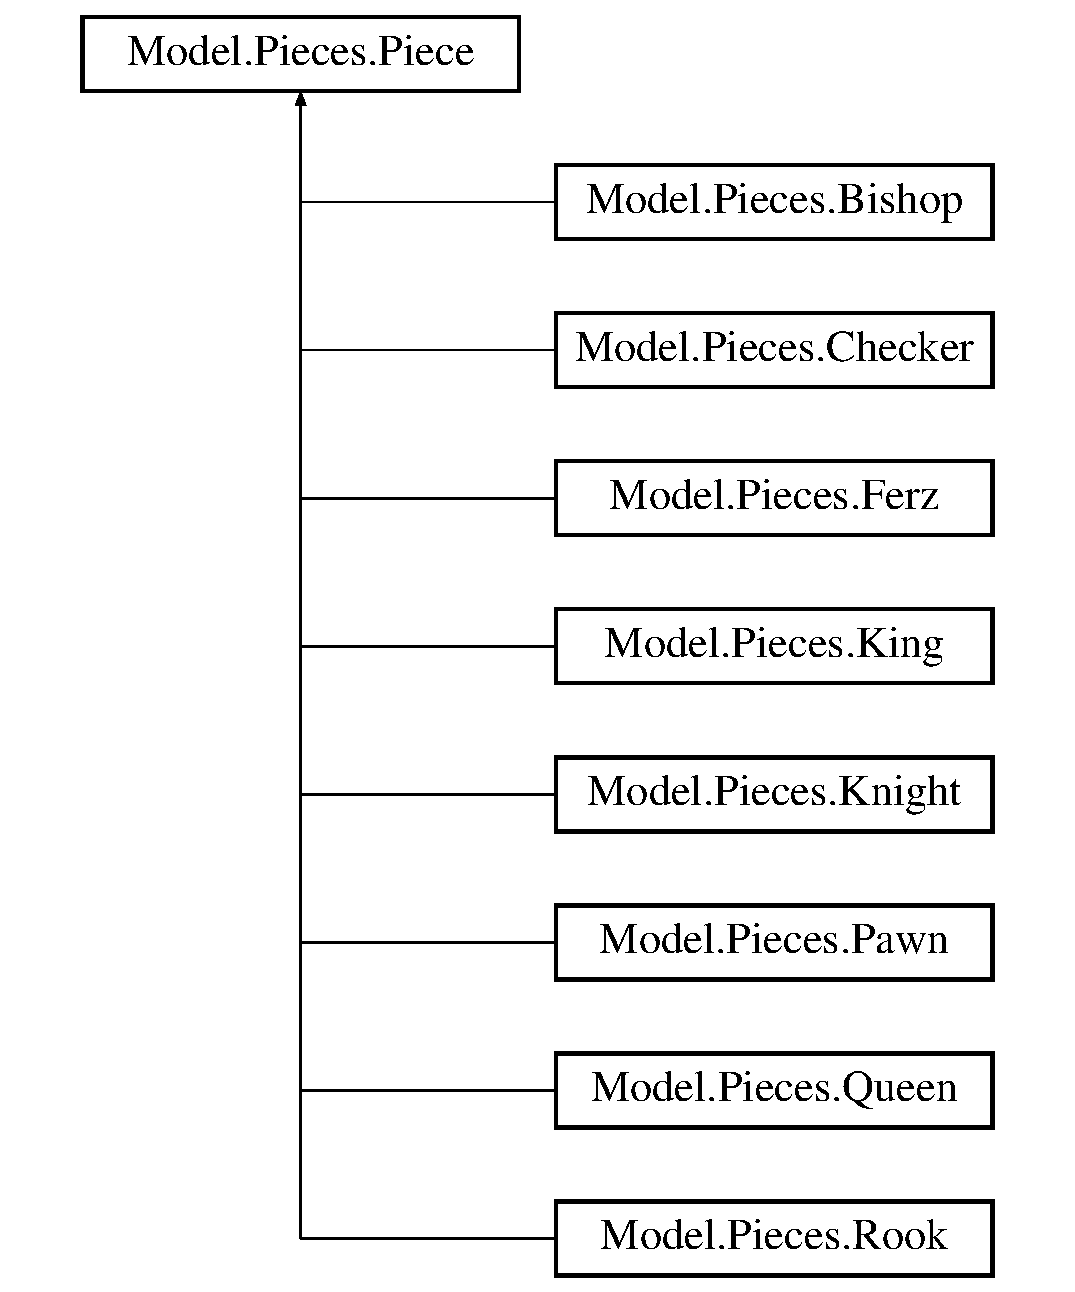
\includegraphics[height=9.000000cm]{class_model_1_1_pieces_1_1_piece}
\end{center}
\end{figure}
\subsection*{Public Member Functions}
\begin{DoxyCompactItemize}
\item 
\hyperlink{class_model_1_1_pieces_1_1_piece_ad2e15ca4e0598c0ff8db23e61bf40ef2}{Piece} (\hyperlink{class_model_1_1_team}{Team} team, int x\+Value, int y\+Value)
\item 
int \hyperlink{class_model_1_1_pieces_1_1_piece_a7390da3b01de7a30694042ad77bd2ee4}{get\+X\+Value} ()
\item 
void \hyperlink{class_model_1_1_pieces_1_1_piece_ae4b44d64ae344e87088a8a36f8742df2}{set\+Coordinates} (int x\+Value, int y\+Value)
\item 
int \hyperlink{class_model_1_1_pieces_1_1_piece_ae211bc6f3f2adf995de3bfa1ab5dfc7b}{get\+Y\+Value} ()
\item 
\hyperlink{class_model_1_1_team}{Team} \hyperlink{class_model_1_1_pieces_1_1_piece_a09296502e0f03fe8d9223060943079ca}{get\+Team} ()
\item 
int \hyperlink{class_model_1_1_pieces_1_1_piece_a86728adbff75375d1b704acfb3dfd994}{get\+Team\+Number} ()
\item 
abstract boolean \hyperlink{class_model_1_1_pieces_1_1_piece_a5415845a97251b8c8da29956769c4f3e}{is\+Valid\+Move} (\hyperlink{class_model_1_1_move}{Move} move, \hyperlink{class_model_1_1_board}{Board} board)
\item 
boolean \hyperlink{class_model_1_1_pieces_1_1_piece_a727ec49c761935c667c5db1279485475}{on\+Available\+Square} (\hyperlink{class_model_1_1_move}{Move} move, \hyperlink{class_model_1_1_board}{Board} board)
\item 
boolean \hyperlink{class_model_1_1_pieces_1_1_piece_a24ae3b8d9b15adcdf3316bfc0afa081c}{traverse\+Row} (int row, int smallX, int bigX, \hyperlink{class_model_1_1_pieces_1_1_piece}{Piece}\mbox{[}$\,$\mbox{]}\mbox{[}$\,$\mbox{]} positions)
\item 
boolean \hyperlink{class_model_1_1_pieces_1_1_piece_a31899e5f9279757bf8a9706df713b4a7}{traverse\+Column} (int column, int smallY, int bigY, \hyperlink{class_model_1_1_pieces_1_1_piece}{Piece}\mbox{[}$\,$\mbox{]}\mbox{[}$\,$\mbox{]} positions)
\item 
boolean \hyperlink{class_model_1_1_pieces_1_1_piece_a37e2c4e79bbcbd2642f79439fd2129a8}{traverse\+Diagonal} (int startX, int endX, int startY, int endY, \hyperlink{class_model_1_1_pieces_1_1_piece}{Piece}\mbox{[}$\,$\mbox{]}\mbox{[}$\,$\mbox{]} positions)
\item 
int \hyperlink{class_model_1_1_pieces_1_1_piece_a236aeb47fd49b23ba097046790554ffc}{get\+Direction} (int start, int end)
\item 
abstract boolean \hyperlink{class_model_1_1_pieces_1_1_piece_a2d3dddd5af8a3d813741d3f6f4e89e10}{has\+No\+Piece\+In\+Movement\+Route} (\hyperlink{class_model_1_1_move}{Move} move, \hyperlink{class_model_1_1_board}{Board} board)
\item 
abstract List$<$ \hyperlink{class_model_1_1_move}{Move} $>$ \hyperlink{class_model_1_1_pieces_1_1_piece_a0f87f230aee0300a8b88570ce7621a36}{find\+All\+Moves} (\hyperlink{class_model_1_1_board}{Board} board)
\item 
List$<$ \hyperlink{class_model_1_1_move}{Move} $>$ \hyperlink{class_model_1_1_pieces_1_1_piece_aa066d5bc9f548630607dca38c9cd0fed}{get\+Moves} (\hyperlink{class_model_1_1_board}{Board} board, int x\+Direction, int y\+Direction, int x\+Value, int y\+Value)
\end{DoxyCompactItemize}


\subsection{Detailed Description}
Parent \hyperlink{class_model_1_1_pieces_1_1_piece}{Piece} Class to hold metadata 

\subsection{Constructor \& Destructor Documentation}
\hypertarget{class_model_1_1_pieces_1_1_piece_ad2e15ca4e0598c0ff8db23e61bf40ef2}{}\label{class_model_1_1_pieces_1_1_piece_ad2e15ca4e0598c0ff8db23e61bf40ef2} 
\index{Model\+::\+Pieces\+::\+Piece@{Model\+::\+Pieces\+::\+Piece}!Piece@{Piece}}
\index{Piece@{Piece}!Model\+::\+Pieces\+::\+Piece@{Model\+::\+Pieces\+::\+Piece}}
\subsubsection{\texorpdfstring{Piece()}{Piece()}}
{\footnotesize\ttfamily Model.\+Pieces.\+Piece.\+Piece (\begin{DoxyParamCaption}\item[{\hyperlink{class_model_1_1_team}{Team}}]{team,  }\item[{int}]{x\+Value,  }\item[{int}]{y\+Value }\end{DoxyParamCaption})}

Constructor that sets piece\textquotesingle{}s team


\begin{DoxyParams}{Parameters}
{\em team\+Number} & \\
\hline
\end{DoxyParams}


\subsection{Member Function Documentation}
\hypertarget{class_model_1_1_pieces_1_1_piece_a0f87f230aee0300a8b88570ce7621a36}{}\label{class_model_1_1_pieces_1_1_piece_a0f87f230aee0300a8b88570ce7621a36} 
\index{Model\+::\+Pieces\+::\+Piece@{Model\+::\+Pieces\+::\+Piece}!find\+All\+Moves@{find\+All\+Moves}}
\index{find\+All\+Moves@{find\+All\+Moves}!Model\+::\+Pieces\+::\+Piece@{Model\+::\+Pieces\+::\+Piece}}
\subsubsection{\texorpdfstring{find\+All\+Moves()}{findAllMoves()}}
{\footnotesize\ttfamily abstract List$<$\hyperlink{class_model_1_1_move}{Move}$>$ Model.\+Pieces.\+Piece.\+find\+All\+Moves (\begin{DoxyParamCaption}\item[{\hyperlink{class_model_1_1_board}{Board}}]{board }\end{DoxyParamCaption})\hspace{0.3cm}{\ttfamily [abstract]}}

Abstract class for pieces to find all moves they can make. 
\begin{DoxyParams}{Parameters}
{\em board} & \\
\hline
\end{DoxyParams}
\begin{DoxyReturn}{Returns}
List of all possible moves in any direction. 
\end{DoxyReturn}
\hypertarget{class_model_1_1_pieces_1_1_piece_a236aeb47fd49b23ba097046790554ffc}{}\label{class_model_1_1_pieces_1_1_piece_a236aeb47fd49b23ba097046790554ffc} 
\index{Model\+::\+Pieces\+::\+Piece@{Model\+::\+Pieces\+::\+Piece}!get\+Direction@{get\+Direction}}
\index{get\+Direction@{get\+Direction}!Model\+::\+Pieces\+::\+Piece@{Model\+::\+Pieces\+::\+Piece}}
\subsubsection{\texorpdfstring{get\+Direction()}{getDirection()}}
{\footnotesize\ttfamily int Model.\+Pieces.\+Piece.\+get\+Direction (\begin{DoxyParamCaption}\item[{int}]{start,  }\item[{int}]{end }\end{DoxyParamCaption})}

Check what direction the movement is in. 
\begin{DoxyParams}{Parameters}
{\em start} & \\
\hline
{\em end} & \\
\hline
\end{DoxyParams}
\begin{DoxyReturn}{Returns}
1 for increasing coordinate, -\/1 for decreasing coordinate 
\end{DoxyReturn}
\hypertarget{class_model_1_1_pieces_1_1_piece_aa066d5bc9f548630607dca38c9cd0fed}{}\label{class_model_1_1_pieces_1_1_piece_aa066d5bc9f548630607dca38c9cd0fed} 
\index{Model\+::\+Pieces\+::\+Piece@{Model\+::\+Pieces\+::\+Piece}!get\+Moves@{get\+Moves}}
\index{get\+Moves@{get\+Moves}!Model\+::\+Pieces\+::\+Piece@{Model\+::\+Pieces\+::\+Piece}}
\subsubsection{\texorpdfstring{get\+Moves()}{getMoves()}}
{\footnotesize\ttfamily List$<$\hyperlink{class_model_1_1_move}{Move}$>$ Model.\+Pieces.\+Piece.\+get\+Moves (\begin{DoxyParamCaption}\item[{\hyperlink{class_model_1_1_board}{Board}}]{board,  }\item[{int}]{x\+Direction,  }\item[{int}]{y\+Direction,  }\item[{int}]{x\+Value,  }\item[{int}]{y\+Value }\end{DoxyParamCaption})}

Function to get all possible moves for a piece in a specific direction according to the current board. 
\begin{DoxyParams}{Parameters}
{\em board} & \\
\hline
{\em x\+Direction} & \\
\hline
{\em y\+Direction} & \\
\hline
{\em x\+Value} & \\
\hline
{\em y\+Value} & \\
\hline
\end{DoxyParams}
\begin{DoxyReturn}{Returns}
All moves possible by a piece in a direction. 
\end{DoxyReturn}
\hypertarget{class_model_1_1_pieces_1_1_piece_a09296502e0f03fe8d9223060943079ca}{}\label{class_model_1_1_pieces_1_1_piece_a09296502e0f03fe8d9223060943079ca} 
\index{Model\+::\+Pieces\+::\+Piece@{Model\+::\+Pieces\+::\+Piece}!get\+Team@{get\+Team}}
\index{get\+Team@{get\+Team}!Model\+::\+Pieces\+::\+Piece@{Model\+::\+Pieces\+::\+Piece}}
\subsubsection{\texorpdfstring{get\+Team()}{getTeam()}}
{\footnotesize\ttfamily \hyperlink{class_model_1_1_team}{Team} Model.\+Pieces.\+Piece.\+get\+Team (\begin{DoxyParamCaption}{ }\end{DoxyParamCaption})}

Get what team this piece is on.

\begin{DoxyReturn}{Returns}
team object 
\end{DoxyReturn}
\hypertarget{class_model_1_1_pieces_1_1_piece_a86728adbff75375d1b704acfb3dfd994}{}\label{class_model_1_1_pieces_1_1_piece_a86728adbff75375d1b704acfb3dfd994} 
\index{Model\+::\+Pieces\+::\+Piece@{Model\+::\+Pieces\+::\+Piece}!get\+Team\+Number@{get\+Team\+Number}}
\index{get\+Team\+Number@{get\+Team\+Number}!Model\+::\+Pieces\+::\+Piece@{Model\+::\+Pieces\+::\+Piece}}
\subsubsection{\texorpdfstring{get\+Team\+Number()}{getTeamNumber()}}
{\footnotesize\ttfamily int Model.\+Pieces.\+Piece.\+get\+Team\+Number (\begin{DoxyParamCaption}{ }\end{DoxyParamCaption})}

Get the piece\textquotesingle{}s team number. \begin{DoxyReturn}{Returns}
team number 
\end{DoxyReturn}
\hypertarget{class_model_1_1_pieces_1_1_piece_a7390da3b01de7a30694042ad77bd2ee4}{}\label{class_model_1_1_pieces_1_1_piece_a7390da3b01de7a30694042ad77bd2ee4} 
\index{Model\+::\+Pieces\+::\+Piece@{Model\+::\+Pieces\+::\+Piece}!get\+X\+Value@{get\+X\+Value}}
\index{get\+X\+Value@{get\+X\+Value}!Model\+::\+Pieces\+::\+Piece@{Model\+::\+Pieces\+::\+Piece}}
\subsubsection{\texorpdfstring{get\+X\+Value()}{getXValue()}}
{\footnotesize\ttfamily int Model.\+Pieces.\+Piece.\+get\+X\+Value (\begin{DoxyParamCaption}{ }\end{DoxyParamCaption})}

Getter for the x coordinate of the piece. \begin{DoxyReturn}{Returns}
X-\/coordinate 
\end{DoxyReturn}
\hypertarget{class_model_1_1_pieces_1_1_piece_ae211bc6f3f2adf995de3bfa1ab5dfc7b}{}\label{class_model_1_1_pieces_1_1_piece_ae211bc6f3f2adf995de3bfa1ab5dfc7b} 
\index{Model\+::\+Pieces\+::\+Piece@{Model\+::\+Pieces\+::\+Piece}!get\+Y\+Value@{get\+Y\+Value}}
\index{get\+Y\+Value@{get\+Y\+Value}!Model\+::\+Pieces\+::\+Piece@{Model\+::\+Pieces\+::\+Piece}}
\subsubsection{\texorpdfstring{get\+Y\+Value()}{getYValue()}}
{\footnotesize\ttfamily int Model.\+Pieces.\+Piece.\+get\+Y\+Value (\begin{DoxyParamCaption}{ }\end{DoxyParamCaption})}

Getter for the y coordinate of the piece. \begin{DoxyReturn}{Returns}
Y-\/\+Coordinate 
\end{DoxyReturn}
\hypertarget{class_model_1_1_pieces_1_1_piece_a2d3dddd5af8a3d813741d3f6f4e89e10}{}\label{class_model_1_1_pieces_1_1_piece_a2d3dddd5af8a3d813741d3f6f4e89e10} 
\index{Model\+::\+Pieces\+::\+Piece@{Model\+::\+Pieces\+::\+Piece}!has\+No\+Piece\+In\+Movement\+Route@{has\+No\+Piece\+In\+Movement\+Route}}
\index{has\+No\+Piece\+In\+Movement\+Route@{has\+No\+Piece\+In\+Movement\+Route}!Model\+::\+Pieces\+::\+Piece@{Model\+::\+Pieces\+::\+Piece}}
\subsubsection{\texorpdfstring{has\+No\+Piece\+In\+Movement\+Route()}{hasNoPieceInMovementRoute()}}
{\footnotesize\ttfamily abstract boolean Model.\+Pieces.\+Piece.\+has\+No\+Piece\+In\+Movement\+Route (\begin{DoxyParamCaption}\item[{\hyperlink{class_model_1_1_move}{Move}}]{move,  }\item[{\hyperlink{class_model_1_1_board}{Board}}]{board }\end{DoxyParamCaption})\hspace{0.3cm}{\ttfamily [abstract]}}

Abstract class for pieces to determine whether there is a piece in the way. 
\begin{DoxyParams}{Parameters}
{\em move} & \\
\hline
{\em board} & \\
\hline
\end{DoxyParams}
\begin{DoxyReturn}{Returns}
Whether the piece jumps over other pieces. 
\end{DoxyReturn}
\hypertarget{class_model_1_1_pieces_1_1_piece_a5415845a97251b8c8da29956769c4f3e}{}\label{class_model_1_1_pieces_1_1_piece_a5415845a97251b8c8da29956769c4f3e} 
\index{Model\+::\+Pieces\+::\+Piece@{Model\+::\+Pieces\+::\+Piece}!is\+Valid\+Move@{is\+Valid\+Move}}
\index{is\+Valid\+Move@{is\+Valid\+Move}!Model\+::\+Pieces\+::\+Piece@{Model\+::\+Pieces\+::\+Piece}}
\subsubsection{\texorpdfstring{is\+Valid\+Move()}{isValidMove()}}
{\footnotesize\ttfamily abstract boolean Model.\+Pieces.\+Piece.\+is\+Valid\+Move (\begin{DoxyParamCaption}\item[{\hyperlink{class_model_1_1_move}{Move}}]{move,  }\item[{\hyperlink{class_model_1_1_board}{Board}}]{board }\end{DoxyParamCaption})\hspace{0.3cm}{\ttfamily [abstract]}}

Check if move is valid


\begin{DoxyParams}{Parameters}
{\em move} & \\
\hline
{\em board} & \\
\hline
\end{DoxyParams}
\begin{DoxyReturn}{Returns}
whether it is valid 
\end{DoxyReturn}
\hypertarget{class_model_1_1_pieces_1_1_piece_a727ec49c761935c667c5db1279485475}{}\label{class_model_1_1_pieces_1_1_piece_a727ec49c761935c667c5db1279485475} 
\index{Model\+::\+Pieces\+::\+Piece@{Model\+::\+Pieces\+::\+Piece}!on\+Available\+Square@{on\+Available\+Square}}
\index{on\+Available\+Square@{on\+Available\+Square}!Model\+::\+Pieces\+::\+Piece@{Model\+::\+Pieces\+::\+Piece}}
\subsubsection{\texorpdfstring{on\+Available\+Square()}{onAvailableSquare()}}
{\footnotesize\ttfamily boolean Model.\+Pieces.\+Piece.\+on\+Available\+Square (\begin{DoxyParamCaption}\item[{\hyperlink{class_model_1_1_move}{Move}}]{move,  }\item[{\hyperlink{class_model_1_1_board}{Board}}]{board }\end{DoxyParamCaption})}

Check if the move goes to an available square that is on the board. 
\begin{DoxyParams}{Parameters}
{\em move} & \\
\hline
{\em board} & \\
\hline
\end{DoxyParams}
\begin{DoxyReturn}{Returns}
true/false whether it is available 
\end{DoxyReturn}
\hypertarget{class_model_1_1_pieces_1_1_piece_ae4b44d64ae344e87088a8a36f8742df2}{}\label{class_model_1_1_pieces_1_1_piece_ae4b44d64ae344e87088a8a36f8742df2} 
\index{Model\+::\+Pieces\+::\+Piece@{Model\+::\+Pieces\+::\+Piece}!set\+Coordinates@{set\+Coordinates}}
\index{set\+Coordinates@{set\+Coordinates}!Model\+::\+Pieces\+::\+Piece@{Model\+::\+Pieces\+::\+Piece}}
\subsubsection{\texorpdfstring{set\+Coordinates()}{setCoordinates()}}
{\footnotesize\ttfamily void Model.\+Pieces.\+Piece.\+set\+Coordinates (\begin{DoxyParamCaption}\item[{int}]{x\+Value,  }\item[{int}]{y\+Value }\end{DoxyParamCaption})}

Setter for both x and y coordinate of the piece after movement. 
\begin{DoxyParams}{Parameters}
{\em x\+Value} & \\
\hline
{\em y\+Value} & \\
\hline
\end{DoxyParams}
\hypertarget{class_model_1_1_pieces_1_1_piece_a31899e5f9279757bf8a9706df713b4a7}{}\label{class_model_1_1_pieces_1_1_piece_a31899e5f9279757bf8a9706df713b4a7} 
\index{Model\+::\+Pieces\+::\+Piece@{Model\+::\+Pieces\+::\+Piece}!traverse\+Column@{traverse\+Column}}
\index{traverse\+Column@{traverse\+Column}!Model\+::\+Pieces\+::\+Piece@{Model\+::\+Pieces\+::\+Piece}}
\subsubsection{\texorpdfstring{traverse\+Column()}{traverseColumn()}}
{\footnotesize\ttfamily boolean Model.\+Pieces.\+Piece.\+traverse\+Column (\begin{DoxyParamCaption}\item[{int}]{column,  }\item[{int}]{smallY,  }\item[{int}]{bigY,  }\item[{\hyperlink{class_model_1_1_pieces_1_1_piece}{Piece}}]{positions\mbox{[}$\,$\mbox{]}\mbox{[}$\,$\mbox{]} }\end{DoxyParamCaption})}

Function to check that there are no pieces being jumped over in the column. 
\begin{DoxyParams}{Parameters}
{\em row} & \\
\hline
{\em smallX} & \\
\hline
{\em bigX} & \\
\hline
{\em positions} & \\
\hline
\end{DoxyParams}
\begin{DoxyReturn}{Returns}
if there are leaps 
\end{DoxyReturn}
\hypertarget{class_model_1_1_pieces_1_1_piece_a37e2c4e79bbcbd2642f79439fd2129a8}{}\label{class_model_1_1_pieces_1_1_piece_a37e2c4e79bbcbd2642f79439fd2129a8} 
\index{Model\+::\+Pieces\+::\+Piece@{Model\+::\+Pieces\+::\+Piece}!traverse\+Diagonal@{traverse\+Diagonal}}
\index{traverse\+Diagonal@{traverse\+Diagonal}!Model\+::\+Pieces\+::\+Piece@{Model\+::\+Pieces\+::\+Piece}}
\subsubsection{\texorpdfstring{traverse\+Diagonal()}{traverseDiagonal()}}
{\footnotesize\ttfamily boolean Model.\+Pieces.\+Piece.\+traverse\+Diagonal (\begin{DoxyParamCaption}\item[{int}]{startX,  }\item[{int}]{endX,  }\item[{int}]{startY,  }\item[{int}]{endY,  }\item[{\hyperlink{class_model_1_1_pieces_1_1_piece}{Piece}}]{positions\mbox{[}$\,$\mbox{]}\mbox{[}$\,$\mbox{]} }\end{DoxyParamCaption})}

Function to check that there are no pieces being jumped over in the diagonal. 
\begin{DoxyParams}{Parameters}
{\em row} & \\
\hline
{\em smallX} & \\
\hline
{\em bigX} & \\
\hline
{\em positions} & \\
\hline
\end{DoxyParams}
\begin{DoxyReturn}{Returns}
if there are leaps 
\end{DoxyReturn}
\hypertarget{class_model_1_1_pieces_1_1_piece_a24ae3b8d9b15adcdf3316bfc0afa081c}{}\label{class_model_1_1_pieces_1_1_piece_a24ae3b8d9b15adcdf3316bfc0afa081c} 
\index{Model\+::\+Pieces\+::\+Piece@{Model\+::\+Pieces\+::\+Piece}!traverse\+Row@{traverse\+Row}}
\index{traverse\+Row@{traverse\+Row}!Model\+::\+Pieces\+::\+Piece@{Model\+::\+Pieces\+::\+Piece}}
\subsubsection{\texorpdfstring{traverse\+Row()}{traverseRow()}}
{\footnotesize\ttfamily boolean Model.\+Pieces.\+Piece.\+traverse\+Row (\begin{DoxyParamCaption}\item[{int}]{row,  }\item[{int}]{smallX,  }\item[{int}]{bigX,  }\item[{\hyperlink{class_model_1_1_pieces_1_1_piece}{Piece}}]{positions\mbox{[}$\,$\mbox{]}\mbox{[}$\,$\mbox{]} }\end{DoxyParamCaption})}

Function to check that there are no pieces being jumped over in the row. 
\begin{DoxyParams}{Parameters}
{\em row} & \\
\hline
{\em smallX} & \\
\hline
{\em bigX} & \\
\hline
{\em positions} & \\
\hline
\end{DoxyParams}
\begin{DoxyReturn}{Returns}
if there are leaps 
\end{DoxyReturn}


The documentation for this class was generated from the following file\+:\begin{DoxyCompactItemize}
\item 
src/\+Model/\+Pieces/Piece.\+java\end{DoxyCompactItemize}

\hypertarget{class_tests_1_1_piece_test}{}\section{Tests.\+Piece\+Test Class Reference}
\label{class_tests_1_1_piece_test}\index{Tests.\+Piece\+Test@{Tests.\+Piece\+Test}}
\subsection*{Public Member Functions}
\begin{DoxyCompactItemize}
\item 
void \hyperlink{class_tests_1_1_piece_test_aa826a8207b7c0c34461cadbd06e86683}{valid\+Constructor} ()  throws Exception 
\item 
void \hyperlink{class_tests_1_1_piece_test_a13e9d2cc31b678368486b03c204408e7}{move\+Off\+Board} ()  throws Exception 
\item 
void \hyperlink{class_tests_1_1_piece_test_af08d686557ed19d88e13e3b3e387ab39}{space\+Occupied\+By\+Same\+Team} ()  throws Exception 
\end{DoxyCompactItemize}


\subsection{Detailed Description}
Tests for the Piece class. \begin{DoxyAuthor}{Author}
arnavmishra 
\end{DoxyAuthor}


\subsection{Member Function Documentation}
\hypertarget{class_tests_1_1_piece_test_a13e9d2cc31b678368486b03c204408e7}{}\label{class_tests_1_1_piece_test_a13e9d2cc31b678368486b03c204408e7} 
\index{Tests\+::\+Piece\+Test@{Tests\+::\+Piece\+Test}!move\+Off\+Board@{move\+Off\+Board}}
\index{move\+Off\+Board@{move\+Off\+Board}!Tests\+::\+Piece\+Test@{Tests\+::\+Piece\+Test}}
\subsubsection{\texorpdfstring{move\+Off\+Board()}{moveOffBoard()}}
{\footnotesize\ttfamily void Tests.\+Piece\+Test.\+move\+Off\+Board (\begin{DoxyParamCaption}{ }\end{DoxyParamCaption}) throws Exception}

Test to confirm that movement off the board is invalid. 
\begin{DoxyExceptions}{Exceptions}
{\em Exception} & \\
\hline
\end{DoxyExceptions}
\hypertarget{class_tests_1_1_piece_test_af08d686557ed19d88e13e3b3e387ab39}{}\label{class_tests_1_1_piece_test_af08d686557ed19d88e13e3b3e387ab39} 
\index{Tests\+::\+Piece\+Test@{Tests\+::\+Piece\+Test}!space\+Occupied\+By\+Same\+Team@{space\+Occupied\+By\+Same\+Team}}
\index{space\+Occupied\+By\+Same\+Team@{space\+Occupied\+By\+Same\+Team}!Tests\+::\+Piece\+Test@{Tests\+::\+Piece\+Test}}
\subsubsection{\texorpdfstring{space\+Occupied\+By\+Same\+Team()}{spaceOccupiedBySameTeam()}}
{\footnotesize\ttfamily void Tests.\+Piece\+Test.\+space\+Occupied\+By\+Same\+Team (\begin{DoxyParamCaption}{ }\end{DoxyParamCaption}) throws Exception}

Test to confirm that a piece cannot move into the same square as a piece of its own team. 
\begin{DoxyExceptions}{Exceptions}
{\em Exception} & \\
\hline
\end{DoxyExceptions}
\hypertarget{class_tests_1_1_piece_test_aa826a8207b7c0c34461cadbd06e86683}{}\label{class_tests_1_1_piece_test_aa826a8207b7c0c34461cadbd06e86683} 
\index{Tests\+::\+Piece\+Test@{Tests\+::\+Piece\+Test}!valid\+Constructor@{valid\+Constructor}}
\index{valid\+Constructor@{valid\+Constructor}!Tests\+::\+Piece\+Test@{Tests\+::\+Piece\+Test}}
\subsubsection{\texorpdfstring{valid\+Constructor()}{validConstructor()}}
{\footnotesize\ttfamily void Tests.\+Piece\+Test.\+valid\+Constructor (\begin{DoxyParamCaption}{ }\end{DoxyParamCaption}) throws Exception}

Test to check the constructor of the Piece class by using a new Pawn\textquotesingle{}s x and y coordinates and team information. 
\begin{DoxyExceptions}{Exceptions}
{\em Exception} & \\
\hline
\end{DoxyExceptions}


The documentation for this class was generated from the following file\+:\begin{DoxyCompactItemize}
\item 
src/\+Tests/Piece\+Test.\+java\end{DoxyCompactItemize}

\hypertarget{class_model_1_1_pieces_1_1_queen}{}\section{Model.\+Pieces.\+Queen Class Reference}
\label{class_model_1_1_pieces_1_1_queen}\index{Model.\+Pieces.\+Queen@{Model.\+Pieces.\+Queen}}
Inheritance diagram for Model.\+Pieces.\+Queen\+:\begin{figure}[H]
\begin{center}
\leavevmode
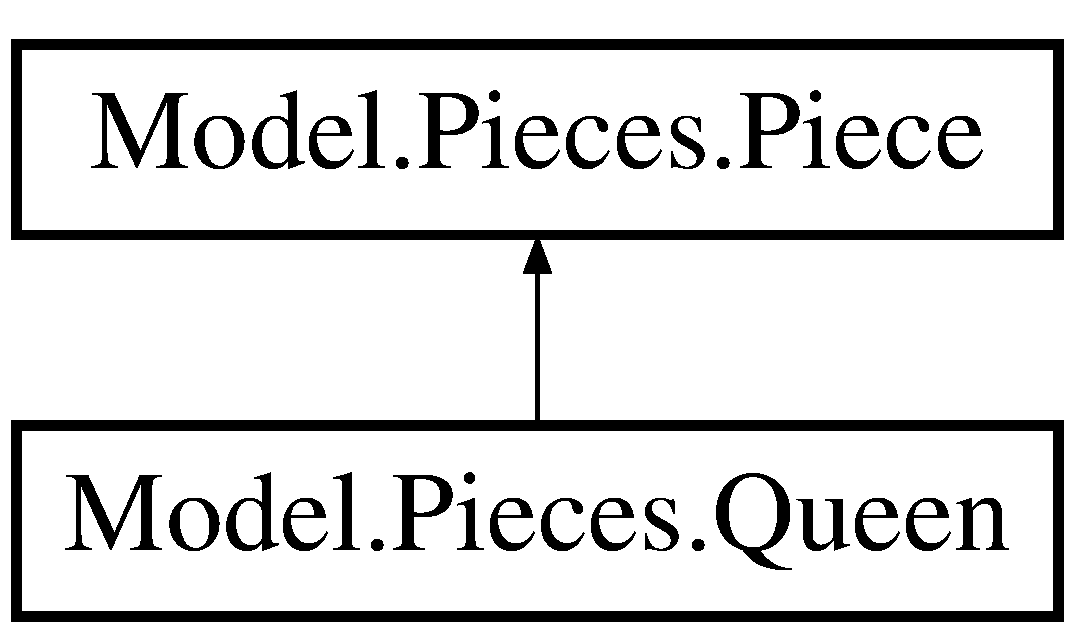
\includegraphics[height=2.000000cm]{class_model_1_1_pieces_1_1_queen}
\end{center}
\end{figure}
\subsection*{Public Member Functions}
\begin{DoxyCompactItemize}
\item 
\hyperlink{class_model_1_1_pieces_1_1_queen_a975dd0d19b30fa943f53e3b8d23a5114}{Queen} (\hyperlink{class_model_1_1_team}{Team} team, int x\+Value, int y\+Value)
\item 
boolean \hyperlink{class_model_1_1_pieces_1_1_queen_a60af220d259d96efdc25e940774fd804}{is\+Valid\+Move} (\hyperlink{class_model_1_1_move}{Move} move, \hyperlink{class_model_1_1_board}{Board} board)
\item 
boolean \hyperlink{class_model_1_1_pieces_1_1_queen_a816cf5f71e321e7a084999db678a01c5}{has\+No\+Piece\+In\+Movement\+Route} (\hyperlink{class_model_1_1_move}{Move} move, \hyperlink{class_model_1_1_board}{Board} board)
\item 
List$<$ \hyperlink{class_model_1_1_move}{Move} $>$ \hyperlink{class_model_1_1_pieces_1_1_queen_ae9cfa3e4e5ebd735f18aed1f66cce4c7}{find\+All\+Moves} (\hyperlink{class_model_1_1_board}{Board} board)
\end{DoxyCompactItemize}


\subsection{Detailed Description}
\hyperlink{class_model_1_1_pieces_1_1_queen}{Queen} class to describe \hyperlink{class_model_1_1_pieces_1_1_queen}{Queen}\textquotesingle{}s possible moves. \begin{DoxyAuthor}{Author}
arnavmishra 
\end{DoxyAuthor}


\subsection{Constructor \& Destructor Documentation}
\hypertarget{class_model_1_1_pieces_1_1_queen_a975dd0d19b30fa943f53e3b8d23a5114}{}\label{class_model_1_1_pieces_1_1_queen_a975dd0d19b30fa943f53e3b8d23a5114} 
\index{Model\+::\+Pieces\+::\+Queen@{Model\+::\+Pieces\+::\+Queen}!Queen@{Queen}}
\index{Queen@{Queen}!Model\+::\+Pieces\+::\+Queen@{Model\+::\+Pieces\+::\+Queen}}
\subsubsection{\texorpdfstring{Queen()}{Queen()}}
{\footnotesize\ttfamily Model.\+Pieces.\+Queen.\+Queen (\begin{DoxyParamCaption}\item[{\hyperlink{class_model_1_1_team}{Team}}]{team,  }\item[{int}]{x\+Value,  }\item[{int}]{y\+Value }\end{DoxyParamCaption})}

Constructor to initialize \hyperlink{class_model_1_1_pieces_1_1_queen}{Queen} on a team and coordinate. 
\begin{DoxyParams}{Parameters}
{\em team} & \\
\hline
\end{DoxyParams}


\subsection{Member Function Documentation}
\hypertarget{class_model_1_1_pieces_1_1_queen_ae9cfa3e4e5ebd735f18aed1f66cce4c7}{}\label{class_model_1_1_pieces_1_1_queen_ae9cfa3e4e5ebd735f18aed1f66cce4c7} 
\index{Model\+::\+Pieces\+::\+Queen@{Model\+::\+Pieces\+::\+Queen}!find\+All\+Moves@{find\+All\+Moves}}
\index{find\+All\+Moves@{find\+All\+Moves}!Model\+::\+Pieces\+::\+Queen@{Model\+::\+Pieces\+::\+Queen}}
\subsubsection{\texorpdfstring{find\+All\+Moves()}{findAllMoves()}}
{\footnotesize\ttfamily List$<$\hyperlink{class_model_1_1_move}{Move}$>$ Model.\+Pieces.\+Queen.\+find\+All\+Moves (\begin{DoxyParamCaption}\item[{\hyperlink{class_model_1_1_board}{Board}}]{board }\end{DoxyParamCaption})}

Function to get all valid possible moves for the \hyperlink{class_model_1_1_pieces_1_1_king}{King} in any direction. 
\begin{DoxyParams}{Parameters}
{\em board} & \\
\hline
\end{DoxyParams}
\begin{DoxyReturn}{Returns}
all possible valid moves. 
\end{DoxyReturn}
\hypertarget{class_model_1_1_pieces_1_1_queen_a816cf5f71e321e7a084999db678a01c5}{}\label{class_model_1_1_pieces_1_1_queen_a816cf5f71e321e7a084999db678a01c5} 
\index{Model\+::\+Pieces\+::\+Queen@{Model\+::\+Pieces\+::\+Queen}!has\+No\+Piece\+In\+Movement\+Route@{has\+No\+Piece\+In\+Movement\+Route}}
\index{has\+No\+Piece\+In\+Movement\+Route@{has\+No\+Piece\+In\+Movement\+Route}!Model\+::\+Pieces\+::\+Queen@{Model\+::\+Pieces\+::\+Queen}}
\subsubsection{\texorpdfstring{has\+No\+Piece\+In\+Movement\+Route()}{hasNoPieceInMovementRoute()}}
{\footnotesize\ttfamily boolean Model.\+Pieces.\+Queen.\+has\+No\+Piece\+In\+Movement\+Route (\begin{DoxyParamCaption}\item[{\hyperlink{class_model_1_1_move}{Move}}]{move,  }\item[{\hyperlink{class_model_1_1_board}{Board}}]{board }\end{DoxyParamCaption})}

The queen can\textquotesingle{}t jump over any pieces since it only moves one space. 
\begin{DoxyParams}{Parameters}
{\em move} & \\
\hline
{\em board} & \\
\hline
\end{DoxyParams}
\begin{DoxyReturn}{Returns}
whether the queen leaps over pieces. 
\end{DoxyReturn}
\hypertarget{class_model_1_1_pieces_1_1_queen_a60af220d259d96efdc25e940774fd804}{}\label{class_model_1_1_pieces_1_1_queen_a60af220d259d96efdc25e940774fd804} 
\index{Model\+::\+Pieces\+::\+Queen@{Model\+::\+Pieces\+::\+Queen}!is\+Valid\+Move@{is\+Valid\+Move}}
\index{is\+Valid\+Move@{is\+Valid\+Move}!Model\+::\+Pieces\+::\+Queen@{Model\+::\+Pieces\+::\+Queen}}
\subsubsection{\texorpdfstring{is\+Valid\+Move()}{isValidMove()}}
{\footnotesize\ttfamily boolean Model.\+Pieces.\+Queen.\+is\+Valid\+Move (\begin{DoxyParamCaption}\item[{\hyperlink{class_model_1_1_move}{Move}}]{move,  }\item[{\hyperlink{class_model_1_1_board}{Board}}]{board }\end{DoxyParamCaption})}

Function to check whether a queen\textquotesingle{}s move is valid. 
\begin{DoxyParams}{Parameters}
{\em move} & \\
\hline
{\em board} & \\
\hline
\end{DoxyParams}
\begin{DoxyReturn}{Returns}
Whether the move is valid. 
\end{DoxyReturn}


The documentation for this class was generated from the following file\+:\begin{DoxyCompactItemize}
\item 
src/\+Model/\+Pieces/Queen.\+java\end{DoxyCompactItemize}

\hypertarget{class_tests_1_1_queen_test}{}\section{Tests.\+Queen\+Test Class Reference}
\label{class_tests_1_1_queen_test}\index{Tests.\+Queen\+Test@{Tests.\+Queen\+Test}}
\subsection*{Public Member Functions}
\begin{DoxyCompactItemize}
\item 
void \hyperlink{class_tests_1_1_queen_test_a8bec252c50587e572eaf3d36fb719d6f}{valid\+Queen\+Forward\+Movement} ()  throws Exception 
\item 
void \hyperlink{class_tests_1_1_queen_test_ae35369361ac4313f3bf86f111479fa75}{valid\+Queen\+Diagonal\+Movement} ()  throws Exception 
\item 
void \hyperlink{class_tests_1_1_queen_test_a0948894af0233e52a11873b7506674bb}{invalid\+Queen\+Movement} ()  throws Exception 
\item 
void \hyperlink{class_tests_1_1_queen_test_a888740ec9527c4998b55eb32bd3c2315}{correct\+All\+Starting\+Queen\+Moves} ()  throws Exception 
\end{DoxyCompactItemize}


\subsection{Detailed Description}
\hyperlink{namespace_tests}{Tests} for the queen class. \begin{DoxyAuthor}{Author}
arnavmishra 
\end{DoxyAuthor}


\subsection{Member Function Documentation}
\hypertarget{class_tests_1_1_queen_test_a888740ec9527c4998b55eb32bd3c2315}{}\label{class_tests_1_1_queen_test_a888740ec9527c4998b55eb32bd3c2315} 
\index{Tests\+::\+Queen\+Test@{Tests\+::\+Queen\+Test}!correct\+All\+Starting\+Queen\+Moves@{correct\+All\+Starting\+Queen\+Moves}}
\index{correct\+All\+Starting\+Queen\+Moves@{correct\+All\+Starting\+Queen\+Moves}!Tests\+::\+Queen\+Test@{Tests\+::\+Queen\+Test}}
\subsubsection{\texorpdfstring{correct\+All\+Starting\+Queen\+Moves()}{correctAllStartingQueenMoves()}}
{\footnotesize\ttfamily void Tests.\+Queen\+Test.\+correct\+All\+Starting\+Queen\+Moves (\begin{DoxyParamCaption}{ }\end{DoxyParamCaption}) throws Exception}

\hyperlink{namespace_tests}{Tests} the queen\textquotesingle{}s list of all possible moves by moving both the pawn in front and the pawn diagonal (up right) out of the way and then checking that the queen can move to all the appropriate locations from there. 
\begin{DoxyExceptions}{Exceptions}
{\em Exception} & \\
\hline
\end{DoxyExceptions}
\hypertarget{class_tests_1_1_queen_test_a0948894af0233e52a11873b7506674bb}{}\label{class_tests_1_1_queen_test_a0948894af0233e52a11873b7506674bb} 
\index{Tests\+::\+Queen\+Test@{Tests\+::\+Queen\+Test}!invalid\+Queen\+Movement@{invalid\+Queen\+Movement}}
\index{invalid\+Queen\+Movement@{invalid\+Queen\+Movement}!Tests\+::\+Queen\+Test@{Tests\+::\+Queen\+Test}}
\subsubsection{\texorpdfstring{invalid\+Queen\+Movement()}{invalidQueenMovement()}}
{\footnotesize\ttfamily void Tests.\+Queen\+Test.\+invalid\+Queen\+Movement (\begin{DoxyParamCaption}{ }\end{DoxyParamCaption}) throws Exception}

\hyperlink{namespace_tests}{Tests} the queen\textquotesingle{}s invalid movement by trying a knight\textquotesingle{}s move for the queen and ensuring that the movement returns as invalid. 
\begin{DoxyExceptions}{Exceptions}
{\em Exception} & \\
\hline
\end{DoxyExceptions}
\hypertarget{class_tests_1_1_queen_test_ae35369361ac4313f3bf86f111479fa75}{}\label{class_tests_1_1_queen_test_ae35369361ac4313f3bf86f111479fa75} 
\index{Tests\+::\+Queen\+Test@{Tests\+::\+Queen\+Test}!valid\+Queen\+Diagonal\+Movement@{valid\+Queen\+Diagonal\+Movement}}
\index{valid\+Queen\+Diagonal\+Movement@{valid\+Queen\+Diagonal\+Movement}!Tests\+::\+Queen\+Test@{Tests\+::\+Queen\+Test}}
\subsubsection{\texorpdfstring{valid\+Queen\+Diagonal\+Movement()}{validQueenDiagonalMovement()}}
{\footnotesize\ttfamily void Tests.\+Queen\+Test.\+valid\+Queen\+Diagonal\+Movement (\begin{DoxyParamCaption}{ }\end{DoxyParamCaption}) throws Exception}

\hyperlink{namespace_tests}{Tests} the queen\textquotesingle{}s diagonal movement by moving the pawn that is diagonal to it (up right) and then moving the queen in that direction. 
\begin{DoxyExceptions}{Exceptions}
{\em Exception} & \\
\hline
\end{DoxyExceptions}
\hypertarget{class_tests_1_1_queen_test_a8bec252c50587e572eaf3d36fb719d6f}{}\label{class_tests_1_1_queen_test_a8bec252c50587e572eaf3d36fb719d6f} 
\index{Tests\+::\+Queen\+Test@{Tests\+::\+Queen\+Test}!valid\+Queen\+Forward\+Movement@{valid\+Queen\+Forward\+Movement}}
\index{valid\+Queen\+Forward\+Movement@{valid\+Queen\+Forward\+Movement}!Tests\+::\+Queen\+Test@{Tests\+::\+Queen\+Test}}
\subsubsection{\texorpdfstring{valid\+Queen\+Forward\+Movement()}{validQueenForwardMovement()}}
{\footnotesize\ttfamily void Tests.\+Queen\+Test.\+valid\+Queen\+Forward\+Movement (\begin{DoxyParamCaption}{ }\end{DoxyParamCaption}) throws Exception}

\hyperlink{namespace_tests}{Tests} the queen\textquotesingle{}s forward movement by moving the pawn in front of it and then moving the queen forward from there. 
\begin{DoxyExceptions}{Exceptions}
{\em Exception} & \\
\hline
\end{DoxyExceptions}


The documentation for this class was generated from the following file\+:\begin{DoxyCompactItemize}
\item 
src/\+Tests/\hyperlink{_queen_test_8java}{Queen\+Test.\+java}\end{DoxyCompactItemize}

\hypertarget{class_model_1_1_pieces_1_1_rook}{}\section{Model.\+Pieces.\+Rook Class Reference}
\label{class_model_1_1_pieces_1_1_rook}\index{Model.\+Pieces.\+Rook@{Model.\+Pieces.\+Rook}}
Inheritance diagram for Model.\+Pieces.\+Rook\+:\begin{figure}[H]
\begin{center}
\leavevmode
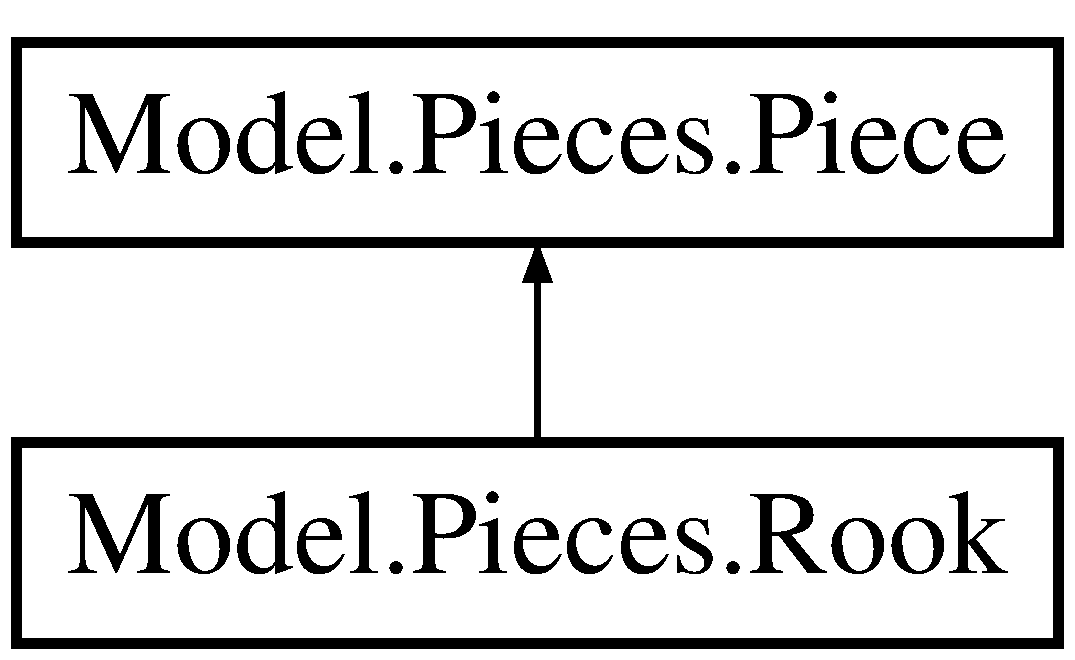
\includegraphics[height=2.000000cm]{class_model_1_1_pieces_1_1_rook}
\end{center}
\end{figure}
\subsection*{Public Member Functions}
\begin{DoxyCompactItemize}
\item 
\hyperlink{class_model_1_1_pieces_1_1_rook_a3e60b56c0706a1a9bb3e02649cc91182}{Rook} (\hyperlink{class_model_1_1_team}{Team} team, int x\+Value, int y\+Value)
\item 
boolean \hyperlink{class_model_1_1_pieces_1_1_rook_a1558998b7bfff64ecd855c210978e1e9}{is\+Valid\+Move} (\hyperlink{class_model_1_1_move}{Move} move, \hyperlink{class_model_1_1_board}{Board} board)
\item 
boolean \hyperlink{class_model_1_1_pieces_1_1_rook_abcd57b340e1eb48e1eca37461373d067}{has\+No\+Piece\+In\+Movement\+Route} (\hyperlink{class_model_1_1_move}{Move} move, \hyperlink{class_model_1_1_board}{Board} board)
\item 
List$<$ \hyperlink{class_model_1_1_move}{Move} $>$ \hyperlink{class_model_1_1_pieces_1_1_rook_adf3f76fc3283bbe0b357e05fd0b3ffb8}{find\+All\+Moves} (\hyperlink{class_model_1_1_board}{Board} board)
\end{DoxyCompactItemize}


\subsection{Detailed Description}
\hyperlink{class_model_1_1_pieces_1_1_rook}{Rook} class to describe \hyperlink{class_model_1_1_pieces_1_1_rook}{Rook}\textquotesingle{}s possible moves. \begin{DoxyAuthor}{Author}
arnavmishra 
\end{DoxyAuthor}


\subsection{Constructor \& Destructor Documentation}
\hypertarget{class_model_1_1_pieces_1_1_rook_a3e60b56c0706a1a9bb3e02649cc91182}{}\label{class_model_1_1_pieces_1_1_rook_a3e60b56c0706a1a9bb3e02649cc91182} 
\index{Model\+::\+Pieces\+::\+Rook@{Model\+::\+Pieces\+::\+Rook}!Rook@{Rook}}
\index{Rook@{Rook}!Model\+::\+Pieces\+::\+Rook@{Model\+::\+Pieces\+::\+Rook}}
\subsubsection{\texorpdfstring{Rook()}{Rook()}}
{\footnotesize\ttfamily Model.\+Pieces.\+Rook.\+Rook (\begin{DoxyParamCaption}\item[{\hyperlink{class_model_1_1_team}{Team}}]{team,  }\item[{int}]{x\+Value,  }\item[{int}]{y\+Value }\end{DoxyParamCaption})}

Constructor to initialize \hyperlink{class_model_1_1_pieces_1_1_rook}{Rook} on a team and coordinate. 
\begin{DoxyParams}{Parameters}
{\em team} & \\
\hline
\end{DoxyParams}


\subsection{Member Function Documentation}
\hypertarget{class_model_1_1_pieces_1_1_rook_adf3f76fc3283bbe0b357e05fd0b3ffb8}{}\label{class_model_1_1_pieces_1_1_rook_adf3f76fc3283bbe0b357e05fd0b3ffb8} 
\index{Model\+::\+Pieces\+::\+Rook@{Model\+::\+Pieces\+::\+Rook}!find\+All\+Moves@{find\+All\+Moves}}
\index{find\+All\+Moves@{find\+All\+Moves}!Model\+::\+Pieces\+::\+Rook@{Model\+::\+Pieces\+::\+Rook}}
\subsubsection{\texorpdfstring{find\+All\+Moves()}{findAllMoves()}}
{\footnotesize\ttfamily List$<$\hyperlink{class_model_1_1_move}{Move}$>$ Model.\+Pieces.\+Rook.\+find\+All\+Moves (\begin{DoxyParamCaption}\item[{\hyperlink{class_model_1_1_board}{Board}}]{board }\end{DoxyParamCaption})}

Function to get all valid possible moves for the \hyperlink{class_model_1_1_pieces_1_1_king}{King} in any direction. 
\begin{DoxyParams}{Parameters}
{\em board} & \\
\hline
\end{DoxyParams}
\begin{DoxyReturn}{Returns}
all possible valid moves. 
\end{DoxyReturn}
\hypertarget{class_model_1_1_pieces_1_1_rook_abcd57b340e1eb48e1eca37461373d067}{}\label{class_model_1_1_pieces_1_1_rook_abcd57b340e1eb48e1eca37461373d067} 
\index{Model\+::\+Pieces\+::\+Rook@{Model\+::\+Pieces\+::\+Rook}!has\+No\+Piece\+In\+Movement\+Route@{has\+No\+Piece\+In\+Movement\+Route}}
\index{has\+No\+Piece\+In\+Movement\+Route@{has\+No\+Piece\+In\+Movement\+Route}!Model\+::\+Pieces\+::\+Rook@{Model\+::\+Pieces\+::\+Rook}}
\subsubsection{\texorpdfstring{has\+No\+Piece\+In\+Movement\+Route()}{hasNoPieceInMovementRoute()}}
{\footnotesize\ttfamily boolean Model.\+Pieces.\+Rook.\+has\+No\+Piece\+In\+Movement\+Route (\begin{DoxyParamCaption}\item[{\hyperlink{class_model_1_1_move}{Move}}]{move,  }\item[{\hyperlink{class_model_1_1_board}{Board}}]{board }\end{DoxyParamCaption})}

The rook can\textquotesingle{}t jump over any pieces since it only moves one space. 
\begin{DoxyParams}{Parameters}
{\em move} & \\
\hline
{\em board} & \\
\hline
\end{DoxyParams}
\begin{DoxyReturn}{Returns}
whether the rook leaps over pieces. 
\end{DoxyReturn}
\hypertarget{class_model_1_1_pieces_1_1_rook_a1558998b7bfff64ecd855c210978e1e9}{}\label{class_model_1_1_pieces_1_1_rook_a1558998b7bfff64ecd855c210978e1e9} 
\index{Model\+::\+Pieces\+::\+Rook@{Model\+::\+Pieces\+::\+Rook}!is\+Valid\+Move@{is\+Valid\+Move}}
\index{is\+Valid\+Move@{is\+Valid\+Move}!Model\+::\+Pieces\+::\+Rook@{Model\+::\+Pieces\+::\+Rook}}
\subsubsection{\texorpdfstring{is\+Valid\+Move()}{isValidMove()}}
{\footnotesize\ttfamily boolean Model.\+Pieces.\+Rook.\+is\+Valid\+Move (\begin{DoxyParamCaption}\item[{\hyperlink{class_model_1_1_move}{Move}}]{move,  }\item[{\hyperlink{class_model_1_1_board}{Board}}]{board }\end{DoxyParamCaption})}

Function to check whether a rook\textquotesingle{}s move is valid. 
\begin{DoxyParams}{Parameters}
{\em move} & \\
\hline
{\em board} & \\
\hline
\end{DoxyParams}
\begin{DoxyReturn}{Returns}
Whether the move is valid. 
\end{DoxyReturn}


The documentation for this class was generated from the following file\+:\begin{DoxyCompactItemize}
\item 
src/\+Model/\+Pieces/Rook.\+java\end{DoxyCompactItemize}

\hypertarget{class_tests_1_1_rook_test}{}\section{Tests.\+Rook\+Test Class Reference}
\label{class_tests_1_1_rook_test}\index{Tests.\+Rook\+Test@{Tests.\+Rook\+Test}}
\subsection*{Public Member Functions}
\begin{DoxyCompactItemize}
\item 
void \hyperlink{class_tests_1_1_rook_test_a3e0f7b9a6c9660eb2a75405197d261d8}{valid\+Vertical\+Rook\+Movement} ()  throws Exception 
\item 
void \hyperlink{class_tests_1_1_rook_test_a668f3fea9c6f61ff4ef09cb0da938810}{valid\+Horizontal\+Rook\+Movement} ()  throws Exception 
\item 
void \hyperlink{class_tests_1_1_rook_test_a3ecbdd2925b2497d7238d3d5057d527e}{invalid\+Rook\+Movement} ()  throws Exception 
\item 
void \hyperlink{class_tests_1_1_rook_test_a63ceffcd172cdbf213102234cddb8580}{correct\+All\+Starting\+Rook\+Moves} ()  throws Exception 
\end{DoxyCompactItemize}


\subsection{Detailed Description}
Tests for the Rook class. \begin{DoxyAuthor}{Author}
arnavmishra 
\end{DoxyAuthor}


\subsection{Member Function Documentation}
\hypertarget{class_tests_1_1_rook_test_a63ceffcd172cdbf213102234cddb8580}{}\label{class_tests_1_1_rook_test_a63ceffcd172cdbf213102234cddb8580} 
\index{Tests\+::\+Rook\+Test@{Tests\+::\+Rook\+Test}!correct\+All\+Starting\+Rook\+Moves@{correct\+All\+Starting\+Rook\+Moves}}
\index{correct\+All\+Starting\+Rook\+Moves@{correct\+All\+Starting\+Rook\+Moves}!Tests\+::\+Rook\+Test@{Tests\+::\+Rook\+Test}}
\subsubsection{\texorpdfstring{correct\+All\+Starting\+Rook\+Moves()}{correctAllStartingRookMoves()}}
{\footnotesize\ttfamily void Tests.\+Rook\+Test.\+correct\+All\+Starting\+Rook\+Moves (\begin{DoxyParamCaption}{ }\end{DoxyParamCaption}) throws Exception}

Test to check all possible moves by the rook by moving the pawn in front of it out of the way and ensuring that the rook can move to the open positions. 
\begin{DoxyExceptions}{Exceptions}
{\em Exception} & \\
\hline
\end{DoxyExceptions}
\hypertarget{class_tests_1_1_rook_test_a3ecbdd2925b2497d7238d3d5057d527e}{}\label{class_tests_1_1_rook_test_a3ecbdd2925b2497d7238d3d5057d527e} 
\index{Tests\+::\+Rook\+Test@{Tests\+::\+Rook\+Test}!invalid\+Rook\+Movement@{invalid\+Rook\+Movement}}
\index{invalid\+Rook\+Movement@{invalid\+Rook\+Movement}!Tests\+::\+Rook\+Test@{Tests\+::\+Rook\+Test}}
\subsubsection{\texorpdfstring{invalid\+Rook\+Movement()}{invalidRookMovement()}}
{\footnotesize\ttfamily void Tests.\+Rook\+Test.\+invalid\+Rook\+Movement (\begin{DoxyParamCaption}{ }\end{DoxyParamCaption}) throws Exception}

Test to check the rook\textquotesingle{}s invalid movement by attempting to move it diagonally and checking that this returns false. 
\begin{DoxyExceptions}{Exceptions}
{\em Exception} & \\
\hline
\end{DoxyExceptions}
\hypertarget{class_tests_1_1_rook_test_a668f3fea9c6f61ff4ef09cb0da938810}{}\label{class_tests_1_1_rook_test_a668f3fea9c6f61ff4ef09cb0da938810} 
\index{Tests\+::\+Rook\+Test@{Tests\+::\+Rook\+Test}!valid\+Horizontal\+Rook\+Movement@{valid\+Horizontal\+Rook\+Movement}}
\index{valid\+Horizontal\+Rook\+Movement@{valid\+Horizontal\+Rook\+Movement}!Tests\+::\+Rook\+Test@{Tests\+::\+Rook\+Test}}
\subsubsection{\texorpdfstring{valid\+Horizontal\+Rook\+Movement()}{validHorizontalRookMovement()}}
{\footnotesize\ttfamily void Tests.\+Rook\+Test.\+valid\+Horizontal\+Rook\+Movement (\begin{DoxyParamCaption}{ }\end{DoxyParamCaption}) throws Exception}

Test to check rook\textquotesingle{}s horizontal movement by moving the pawn in front of it out of the way, moving the rook forward, and then moving the rook to the right for the horizontal movement. 
\begin{DoxyExceptions}{Exceptions}
{\em Exception} & \\
\hline
\end{DoxyExceptions}
\hypertarget{class_tests_1_1_rook_test_a3e0f7b9a6c9660eb2a75405197d261d8}{}\label{class_tests_1_1_rook_test_a3e0f7b9a6c9660eb2a75405197d261d8} 
\index{Tests\+::\+Rook\+Test@{Tests\+::\+Rook\+Test}!valid\+Vertical\+Rook\+Movement@{valid\+Vertical\+Rook\+Movement}}
\index{valid\+Vertical\+Rook\+Movement@{valid\+Vertical\+Rook\+Movement}!Tests\+::\+Rook\+Test@{Tests\+::\+Rook\+Test}}
\subsubsection{\texorpdfstring{valid\+Vertical\+Rook\+Movement()}{validVerticalRookMovement()}}
{\footnotesize\ttfamily void Tests.\+Rook\+Test.\+valid\+Vertical\+Rook\+Movement (\begin{DoxyParamCaption}{ }\end{DoxyParamCaption}) throws Exception}

Test to check the rook\textquotesingle{}s vertical movement by moving the pawn in front of it out of the way and then moving the rook forward. 
\begin{DoxyExceptions}{Exceptions}
{\em Exception} & \\
\hline
\end{DoxyExceptions}


The documentation for this class was generated from the following file\+:\begin{DoxyCompactItemize}
\item 
src/\+Tests/Rook\+Test.\+java\end{DoxyCompactItemize}

\hypertarget{class_model_1_1_team}{}\section{Model.\+Team Class Reference}
\label{class_model_1_1_team}\index{Model.\+Team@{Model.\+Team}}
\subsection*{Public Member Functions}
\begin{DoxyCompactItemize}
\item 
\hyperlink{class_model_1_1_team_a812b4a8f7c7facaec72a7c9b9f16d72c}{Team} (int team\+Number)
\item 
int \hyperlink{class_model_1_1_team_a2e60ec224f46ae7d0b682bdba79a1d85}{get\+Team\+Number} ()
\item 
void \hyperlink{class_model_1_1_team_ae29f91cb29d72c68f8e1d97b08d86eb4}{add\+Pieces} (\hyperlink{class_model_1_1_pieces_1_1_piece}{Piece}\mbox{[}$\,$\mbox{]} piece)
\item 
void \hyperlink{class_model_1_1_team_ab9243a9d3a778a57d4d25c9238b069f7}{add\+Piece} (\hyperlink{class_model_1_1_pieces_1_1_piece}{Piece} piece)
\item 
void \hyperlink{class_model_1_1_team_ad0e67548dd19712a5be9672c7d9b6d0e}{remove\+Piece} (\hyperlink{class_model_1_1_pieces_1_1_piece}{Piece} piece)
\item 
List$<$ \hyperlink{class_model_1_1_pieces_1_1_piece}{Piece} $>$ \hyperlink{class_model_1_1_team_a3abaa196ae93d5a51e3beca8c94bec76}{get\+Pieces} ()
\end{DoxyCompactItemize}


\subsection{Detailed Description}
\hyperlink{class_model_1_1_team}{Team} class to hold metadata about each team. \begin{DoxyAuthor}{Author}
arnavmishra 
\end{DoxyAuthor}


\subsection{Constructor \& Destructor Documentation}
\hypertarget{class_model_1_1_team_a812b4a8f7c7facaec72a7c9b9f16d72c}{}\label{class_model_1_1_team_a812b4a8f7c7facaec72a7c9b9f16d72c} 
\index{Model\+::\+Team@{Model\+::\+Team}!Team@{Team}}
\index{Team@{Team}!Model\+::\+Team@{Model\+::\+Team}}
\subsubsection{\texorpdfstring{Team()}{Team()}}
{\footnotesize\ttfamily Model.\+Team.\+Team (\begin{DoxyParamCaption}\item[{int}]{team\+Number }\end{DoxyParamCaption})}

Constructor to initialize team with a team number. 
\begin{DoxyParams}{Parameters}
{\em team\+Number} & \\
\hline
\end{DoxyParams}


\subsection{Member Function Documentation}
\hypertarget{class_model_1_1_team_ab9243a9d3a778a57d4d25c9238b069f7}{}\label{class_model_1_1_team_ab9243a9d3a778a57d4d25c9238b069f7} 
\index{Model\+::\+Team@{Model\+::\+Team}!add\+Piece@{add\+Piece}}
\index{add\+Piece@{add\+Piece}!Model\+::\+Team@{Model\+::\+Team}}
\subsubsection{\texorpdfstring{add\+Piece()}{addPiece()}}
{\footnotesize\ttfamily void Model.\+Team.\+add\+Piece (\begin{DoxyParamCaption}\item[{\hyperlink{class_model_1_1_pieces_1_1_piece}{Piece}}]{piece }\end{DoxyParamCaption})}

Adds a single piece to the active piece list for the team. 
\begin{DoxyParams}{Parameters}
{\em piece} & \\
\hline
\end{DoxyParams}
\hypertarget{class_model_1_1_team_ae29f91cb29d72c68f8e1d97b08d86eb4}{}\label{class_model_1_1_team_ae29f91cb29d72c68f8e1d97b08d86eb4} 
\index{Model\+::\+Team@{Model\+::\+Team}!add\+Pieces@{add\+Pieces}}
\index{add\+Pieces@{add\+Pieces}!Model\+::\+Team@{Model\+::\+Team}}
\subsubsection{\texorpdfstring{add\+Pieces()}{addPieces()}}
{\footnotesize\ttfamily void Model.\+Team.\+add\+Pieces (\begin{DoxyParamCaption}\item[{\hyperlink{class_model_1_1_pieces_1_1_piece}{Piece} \mbox{[}$\,$\mbox{]}}]{piece }\end{DoxyParamCaption})}

Adds an array of pieces to the active piece list for the team. 
\begin{DoxyParams}{Parameters}
{\em piece} & \\
\hline
\end{DoxyParams}
\hypertarget{class_model_1_1_team_a3abaa196ae93d5a51e3beca8c94bec76}{}\label{class_model_1_1_team_a3abaa196ae93d5a51e3beca8c94bec76} 
\index{Model\+::\+Team@{Model\+::\+Team}!get\+Pieces@{get\+Pieces}}
\index{get\+Pieces@{get\+Pieces}!Model\+::\+Team@{Model\+::\+Team}}
\subsubsection{\texorpdfstring{get\+Pieces()}{getPieces()}}
{\footnotesize\ttfamily List$<$\hyperlink{class_model_1_1_pieces_1_1_piece}{Piece}$>$ Model.\+Team.\+get\+Pieces (\begin{DoxyParamCaption}{ }\end{DoxyParamCaption})}

Getter for the pieces of the team. \begin{DoxyReturn}{Returns}

\end{DoxyReturn}
\hypertarget{class_model_1_1_team_a2e60ec224f46ae7d0b682bdba79a1d85}{}\label{class_model_1_1_team_a2e60ec224f46ae7d0b682bdba79a1d85} 
\index{Model\+::\+Team@{Model\+::\+Team}!get\+Team\+Number@{get\+Team\+Number}}
\index{get\+Team\+Number@{get\+Team\+Number}!Model\+::\+Team@{Model\+::\+Team}}
\subsubsection{\texorpdfstring{get\+Team\+Number()}{getTeamNumber()}}
{\footnotesize\ttfamily int Model.\+Team.\+get\+Team\+Number (\begin{DoxyParamCaption}{ }\end{DoxyParamCaption})}

Getter for team\textquotesingle{}s number. \begin{DoxyReturn}{Returns}

\end{DoxyReturn}
\hypertarget{class_model_1_1_team_ad0e67548dd19712a5be9672c7d9b6d0e}{}\label{class_model_1_1_team_ad0e67548dd19712a5be9672c7d9b6d0e} 
\index{Model\+::\+Team@{Model\+::\+Team}!remove\+Piece@{remove\+Piece}}
\index{remove\+Piece@{remove\+Piece}!Model\+::\+Team@{Model\+::\+Team}}
\subsubsection{\texorpdfstring{remove\+Piece()}{removePiece()}}
{\footnotesize\ttfamily void Model.\+Team.\+remove\+Piece (\begin{DoxyParamCaption}\item[{\hyperlink{class_model_1_1_pieces_1_1_piece}{Piece}}]{piece }\end{DoxyParamCaption})}

Removes a piece from the array of pieces after capture. 
\begin{DoxyParams}{Parameters}
{\em piece} & \\
\hline
\end{DoxyParams}


The documentation for this class was generated from the following file\+:\begin{DoxyCompactItemize}
\item 
src/\+Model/Team.\+java\end{DoxyCompactItemize}

\hypertarget{class_tests_1_1_team_test}{}\section{Tests.\+Team\+Test Class Reference}
\label{class_tests_1_1_team_test}\index{Tests.\+Team\+Test@{Tests.\+Team\+Test}}
\subsection*{Public Member Functions}
\begin{DoxyCompactItemize}
\item 
void \hyperlink{class_tests_1_1_team_test_a2e81c6940e0a7ed7ec9f05ea4d0799d7}{valid\+Constructor} ()  throws Exception 
\item 
void \hyperlink{class_tests_1_1_team_test_a7cb853699e49ed8f2cb52056fba9be1e}{take\+A\+Piece} ()  throws Exception 
\item 
void \hyperlink{class_tests_1_1_team_test_a7a58d153f2570b724ee30b0281387739}{add\+A\+Piece} ()  throws Exception 
\end{DoxyCompactItemize}


\subsection{Detailed Description}
Tests for the Team class. \begin{DoxyAuthor}{Author}
arnavmishra 
\end{DoxyAuthor}


\subsection{Member Function Documentation}
\hypertarget{class_tests_1_1_team_test_a7a58d153f2570b724ee30b0281387739}{}\label{class_tests_1_1_team_test_a7a58d153f2570b724ee30b0281387739} 
\index{Tests\+::\+Team\+Test@{Tests\+::\+Team\+Test}!add\+A\+Piece@{add\+A\+Piece}}
\index{add\+A\+Piece@{add\+A\+Piece}!Tests\+::\+Team\+Test@{Tests\+::\+Team\+Test}}
\subsubsection{\texorpdfstring{add\+A\+Piece()}{addAPiece()}}
{\footnotesize\ttfamily void Tests.\+Team\+Test.\+add\+A\+Piece (\begin{DoxyParamCaption}{ }\end{DoxyParamCaption}) throws Exception}

Test of adding a new piece to a team. The test adds a pawn and confirms that there are now 9 pawns instead of 8. 
\begin{DoxyExceptions}{Exceptions}
{\em Exception} & \\
\hline
\end{DoxyExceptions}
\hypertarget{class_tests_1_1_team_test_a7cb853699e49ed8f2cb52056fba9be1e}{}\label{class_tests_1_1_team_test_a7cb853699e49ed8f2cb52056fba9be1e} 
\index{Tests\+::\+Team\+Test@{Tests\+::\+Team\+Test}!take\+A\+Piece@{take\+A\+Piece}}
\index{take\+A\+Piece@{take\+A\+Piece}!Tests\+::\+Team\+Test@{Tests\+::\+Team\+Test}}
\subsubsection{\texorpdfstring{take\+A\+Piece()}{takeAPiece()}}
{\footnotesize\ttfamily void Tests.\+Team\+Test.\+take\+A\+Piece (\begin{DoxyParamCaption}{ }\end{DoxyParamCaption}) throws Exception}

Test to confirm that when an opposing team takes a piece from a Team, the list of pieces works updates accordingly. In this situation, a pawn is taken from the team and there are only 7 pawns left after. 
\begin{DoxyExceptions}{Exceptions}
{\em Exception} & \\
\hline
\end{DoxyExceptions}
\hypertarget{class_tests_1_1_team_test_a2e81c6940e0a7ed7ec9f05ea4d0799d7}{}\label{class_tests_1_1_team_test_a2e81c6940e0a7ed7ec9f05ea4d0799d7} 
\index{Tests\+::\+Team\+Test@{Tests\+::\+Team\+Test}!valid\+Constructor@{valid\+Constructor}}
\index{valid\+Constructor@{valid\+Constructor}!Tests\+::\+Team\+Test@{Tests\+::\+Team\+Test}}
\subsubsection{\texorpdfstring{valid\+Constructor()}{validConstructor()}}
{\footnotesize\ttfamily void Tests.\+Team\+Test.\+valid\+Constructor (\begin{DoxyParamCaption}{ }\end{DoxyParamCaption}) throws Exception}

Test to check the constructor by ensuring that a Team\textquotesingle{}s team\+Number is set properly. 
\begin{DoxyExceptions}{Exceptions}
{\em Exception} & \\
\hline
\end{DoxyExceptions}


The documentation for this class was generated from the following file\+:\begin{DoxyCompactItemize}
\item 
src/\+Tests/Team\+Test.\+java\end{DoxyCompactItemize}

%--- End generated contents ---

% Index
\backmatter
\newpage
\phantomsection
\clearemptydoublepage
\addcontentsline{toc}{chapter}{Index}
\printindex

\end{document}
